\documentclass[a4paper,justified,notoc]{tufte-book}

\setcounter{secnumdepth}{2}
\renewcommand{\contentsname}{Sisältö}

\titleformat{\chapter}{\Huge\rmfamily\scshape}{\thechapter}{18pt}{\Huge\rmfamily\scshape}
\titleformat{\section}{\huge\rmfamily}{\thesection}{12pt}{\huge\rmfamily}
\titleformat{\subsection}{\Large\bfseries}{\thesubsection}{9pt}{\Large\bfseries}

\hypersetup{colorlinks}

%%
% Omat komennot
\newcommand{\lut}{Lappeenrannan-Lahden teknillinen yliopisto LUT }
\newcommand{\lutin}{Lappeenrannan-Lahden teknillisen yliopiston LUT:n }
\newcommand{\eng}[1]{\textit{(#1)}}
\newcommand{\new}[1]{\textit{\gls{#1}}}
\newcommand{\newnogls}[1]{\textit{#1}}
\newcommand{\neweng}[2]{\new{#1} \eng{#2}}
\newcommand{\newengnogls}[2]{\newnogls{#1} \eng{#2}}
\newcommand{\java}[1]{\underline{\gls{java:#1}}}
\newcommand{\javanogls}[1]{\underline{#1}}
\newcommand{\newjava}[1]{\textit{\java{#1}}}
\newcommand{\newjavanogls}[1]{\textit{\javanogls{#1}}}


%%
% Book metadata
\title{Ohjelmointiopas{\small \lutin olio-ohjelmointikurssi}\thanks{Kiitokset kandityön valvojalle
Erno Vanhalalle.}}
\author[Eetu Juhani Asikainen]{Eetu Juhani Asikainen}
\publisher{BETA}

%%
% For nicely typeset tabular material
\usepackage{booktabs}

\usepackage[utf8]{inputenc}

%%
% Prints a trailing space in a smart way.
\usepackage{xspace}

% Prints the month name (e.g., January) and the year (e.g., 2008)
\newcommand{\monthyear}{
  \ifcase\month\or January\or February\or March\or April\or May\or June\or
  July\or August\or September\or October\or November\or
  December\fi\space\number\year
}

\usepackage{units}
\usepackage{graphicx}
\graphicspath{{./Kuvat/}}

% Generates the index
\usepackage{makeidx}
\makeindex

\usepackage{titletoc}
\usepackage{etoolbox}
\setcounter{tocdepth}{2}

\usepackage[toc, automake]{glossaries}
\newglossary[jvg]{java}{jvd}{jvn}{Javan avainsanat}
\glsaddall
\makeglossaries

%%%%%%%%%%%%%%%%%%%%%%%%%%%%%%%%%%%%%%%%%%%%%%%%%%%%%%%%%%%%%%%%%%%%%%%%%%%%%%%%%%%%%%%%%%%%%%%%%%
% % % % % % % % % % % % % % % % % % % % % % % % % % % % % % % % % % % % % % % % % % % % % % % % %
%%%%%%%%%%%%%%%%%%%%%%%%%%%%%%%%%%%%%%%%%%%%%%%%%%%%%%%%%%%%%%%%%%%%%%%%%%%%%%%%%%%%%%%%%%%%%%%%%%

\usepackage[newfloat]{minted}
\usepackage{caption}

\newenvironment{code_example}{\captionsetup{type=listing}}{}
\SetupFloatingEnvironment{listing}{name=Koodiesimerkki}

\newcommand{\code}[3]{
	\begin{code_example}
		\captionof{listing}{#1: #3}
		\label{code_example:#1/#2}
		\inputminted{java}{OhjelmointiopasEsimerkit/src/#1/#2.java}
	\end{code_example}
}

\renewcommand*{\listlistingname}{Oppaan koodiesimerkit}

%%%%%%%%%%%%%%%%%%%%%%%%%%%%%%%%%%%%%%%%%%%%%%%%%%%%%%%%%%%%%%%%%%%%%%%%%%%%%%%%%%%%%%%%%%%%%%%%%%
% % % % % % % % % % % % % % % % % % % % % % % % % % % % % % % % % % % % % % % % % % % % % % % % %
%%%%%%%%%%%%%%%%%%%%%%%%%%%%%%%%%%%%%%%%%%%%%%%%%%%%%%%%%%%%%%%%%%%%%%%%%%%%%%%%%%%%%%%%%%%%%%%%%%

%% SANASTOT
\newglossaryentry{abstraktio}
{
    name=abstraktio,
    description={(abstraction) Ohjelmoinnin perustekniikka, jossa ongelman
tarkka ratkaisu piilotetaan kutsuttavan koodirakenteen, kuten funktion, 
tietorakenteen tai luokan taakse}
}

\newglossaryentry{funktio}
{
    name=funktio,
    description={(function) Ohjelmoijan määrittelemä käskysarja, eli koodin
osa, joka on rajattu, ottaa tietyn määrän parametreja ja mahdollisesti
palauttaa paluuarvon. Tunnetaan olio-ohjelmoinnissa nimellä metodi},
    see={parametri,metodi}
}

\newglossaryentry{parametri}
{
    name=parametri,
    description={(parameter) Arvo, jonka funktio tai metodi ottaa muulta
koodilta vastaan},
    see={funktio,metodi}
}

\newglossaryentry{metodi}
{
    name=metodi,
    description={(method) Luokkaan sidottu käskysarja, joka suorittaa
ottamiensa parametrien ja luokan omien datakenttien perusteella jonkin tietyn
toiminnon},
    see={parametri,funktio,luokka}
}

\newglossaryentry{tietue}
{
    name=tietue,
    description={(struct) Vanhahko muokattava tietotyyppi, yleinen esimerkiksi
C-kielessä. Käyttäjä voi määritellä tietueen sisältämään mitä tahansa
vakiokokoisia datakenttiä. Luokkien edeltäjä}
}

\newglossaryentry{olio}
{
    name=olio,
    description={(object) Luokan instanssi. Yksittäinen koodissa luotu
toimija, joka sisältää datakenttiä ja metodeita. Luokka, jonka pohjalta olio
luodaan määrittää olion käytettävissä olevat metodit ja siihen
tallennetut datatyypit, mutta vain olio pääsee käsiksi omiin metodeihin
ja datakenttiinsä},
    see={luokka,metodi,instanssi}
}

\newglossaryentry{luokka}
{
    name=luokka,
    description={(class) Ohjelmoijan kirjoittama muotti, jonka pohjalta
ohjelmisto luo olioita. Voi sisältää metodeja ja datakenttiä mutta yleensä
näiden käyttämiseksi vaaditaan olion luontia},
    see={olio,metodi,instanssi}
}

\newglossaryentry{instanssi}
{
    name=instanssi,
    description={(instance) Olio, joka on luotu jonkin luokan pohjalta on
kyseisen luokan instanssi},
    see={olio,luokka}
}

\newglossaryentry{enkapsulaatio}
{
    name=enkapsulaatio,
    description={(encapsulation) Datan piilottaminen olion sisään niin ettei
muu ohjelmisto näe kyseistä dataa. Mitataan asteikolla matala-korkea, niin että
korkea enkapsulaatio tarkoittaa pientä määrää julkisia metodeja tai datakenttiä
ja matala taas suurta määrää julkisia metodeja ja datakenttiä}
    see={luokka,koheesio,metodi}
}

\newglossaryentry{rajapinta}
{
    name=rajapinta,
    description={(interface) Yleisessä käytössä termi ohjelmistossa toteutuvalle sopimukselle,
jonka jokin metodi, luokka tmv. toteuttaa tai kahden ohjelmiston osan välinen taso. Javan
yhteydessä luokka, joka luodaan interface-avainsanalla ja joka sisältää vain
luokan implementoimien metodien signatuurit. Rajapintaluokka ei yleensä sisällä ollenkaan
toiminnallista koodia},
    see={java:interface}
}

\newglossaryentry{koheesio}
{
    name=koheesio,
    description={(cohesion) Ohjelmiston laadun mittaamiseen käytetty käsite.
Mittaa luokkien sisäistä yhtenäisyyttä akselilla matala-korkea. Matala koheesio
tarkoittaa että luokassa on paljon metodeja jotka eivät keskustele toisten
luokan metodien kanssa ja matala että luokan kaikki metodit käyttävät useita
muita luokan metodeja. Matala koheesio on toivottavaa, koska luokan tehtävä
on tehdä yksi ja vain yksi asia}
}

\newglossaryentry{pariutuminen}
{
    name=pariutuminen,
    description={(coupling) Ohjelman laadun mittaamiseen käytetty käsite.
Mittaa luokkien keskenäisten riippuvuuksien määrää akselilla löysä-tiukka.
Löysässä pariutumisessa ohjelmiston luokkien väliset riippuvuudet ovat
harvassa, jolloin ohjelmiston muokkaaminen on helppoa. Tiukassa pariutumisessa
puolestaan jokaisella ohjelmiston luokalla on riippuvuus moneen muuhun
ohjelmiston luokkaan, jolloin ohjelmison muokkaus hankaloituu ja täten voidaan
katsoa ohjelmiston laadun laskevan}
}

\newglossaryentry{primitiivinen tietotyyppi}{
    name=primitiivinen tietotyyppi,
    description={(primitive data type) Tietotyyppi, jonka ohjelmointikieli
kykenee säilömään suoraan muistipaikkaan raakana numeerisena datana. Ainoat
tietotyypit Javassa, jotka eivät ole jonkin luokan instansseja},
    see={luokka,instanssi}
}

\newglossaryentry{nakyvyysmaare}
{
    name=näkyvyysmääre,
    description={(access modifier) Muuttujan näkyvyyden määrittävä avainsana},
    see=muuttuja
}

\newglossaryentry{muuttuja}
{
    name=muuttuja,
    description={(variable) koodissa määritelty tietokenttä, joka sisältää jonkin ohjelman
käyttämän arvon}
}

\newglossaryentry{staattinen kieli}
{
    name=staattisesti tyypitetty kieli,
    description={(statically typed language) Ohjelmointikieli, joka tietää jokaisen koodissa
esiintyvän muuttujan tietotyypin koko ajan}
}

\newglossaryentry{signatuuri}
{
	name=signatuuri,
	description={(signature) Metodin määritelmä, joka sisältää sekä metodin nimen, että sen
ottamien argumenttien tyypit}
}

\newglossaryentry{noutaja}
{
	name=noutaja,
	description={(getter) Metodi, jonka tehtävänä on tarjota rajoitettu saatavuus johonkin
luokan yksityiseen muuttujan. Ei yleensä ota argumentteja ja palauttaa luokan omistaman toivotun
muuttujan. Nimetään camelCase-tyylillä sijoittamalla muuttujan nimen eteen "get" ("getVariable").
Parantaa enkapsulaatiota ja mahdollistaa esimerkiksi laiskan alustuksen muuttujille}
}

\newglossaryentry{asettaja}
{
	name=asettaja,
	description={(setter) Metodi, jonka tehtävänä on tarjota luokan ulkopuolisille toimijoille
mahdollisuus asettaa arvoja luokan yksityiseen muuttujaan. Ottaa yleensä arvoksi muuttujan toivotun
arvon, eikä palauta mitään. Nimetään camelCase-tyylillä sijoittamalla muuttujan nimen eteen "set"
("setVariable"). Parantaa enkapsulaatiota ja mahdollistaa esimerkiksi uusien arvojen validoinnin
ennen niiden asettamista}
}

\newglossaryentry{rakentaja}
{
	name=rakentaja,
	description={(constructor) Luokkametodi, joka määritellään ja kutsutaan luokan nimellä ja nimensä
mukaisesti rakentaa ja palauttaa uuden luokan instanssin},
	see={luokkametodi,instanssi,java:new}
}

\newglossaryentry{luokkametodi}
{
	name=luokkametodi,
	description={(class method) Metodi, joka on luokan instanssin sijaan sidottu itse luokkaan.
Ei voida käyttää instanssiin sidottuja muuttujia, mutta voi käyttää luokkamuuttujia. Määritellään
yleensä static-avainsanalla ja kutsutaan luokan nimen pistenotaatiolla},
	see={luokkamuuttuja,java:static}
}

\newglossaryentry{luokkamuuttuja}
{
	name=luokkamuuttuja,
	description={(class variable) Muuttuja, joka on luokan instanssin sijaan sidottu itse luokkaan.
Muokattavissa ja tarkasteltavissa jokaisesta luokan instanssista jaetusti. Määritellään yleensä
static-avainsanalla},
	see=java:static
}

\newglossaryentry{taulukko}
{
	name=taulukko,
	description={(array) Tietorakenne, jossa yksittäiset alkiot on säilötty vierekkäisiin
muistipaikkoihin. Vie vähän muistitilaa ja mahdollistaa nopeat haut ja lisäykset jos alkion
indeksi on tiedossa etukäteen. Yleensä taulukon koko on määriteltävä sen luomisen yhteydessä,
tämä on totta myös Javassa. Javassa taulukko luodaan new-avainsanalla lisäämällä taulukon
säilömän tietotyypin perään hakasulkeet, joiden sisään suljetaan taulukon koon määrittelevä
numero. Taulukkotyyppinen muuttuja määritellään lisäämällä muuttujan tietotyypin määritelmän
perään hakasulkeet. Tällöin esimerkiksi int-tyypin kymmenen alkion taulukko, joka on säilötty
"intArray"-muuttujaan määriteltäisiin seuraavasti:\newline{} "int[] intArray = new int[10]"}
}

\newglossaryentry{geneerinen luokka}
{
	name=geneerinen luokka,
	description={(generic class) Luokan ominaisuus, joka määrittää luokan instanssien täyden
tyyppisignatuurin olevan riippuvainen toisesta luokasta. Tämä toinen luokka voidaan määrittää
jokaisen luokan instanssin kohdalla erikseen pienempi kuin- ja suurempi kuin -merkkien väliin
suljetulla notaatiolla. Esimerkiksi kokoelmat tarvitsevat tietoa sisältämiensä olioiden
tyypityksestä. Merkkijonoja sisältävä ArrayList-kokoelma voitaisiin siis luoda seuraavalla 
notaatiolla:\newline{}"new ArrayList<String>()"\newline{}Geneerinen luokka voi olla myös geneerinen useamman luokan suhteen, jolloin luokat erotetaan pilkulla tai riippuvainen toisesta
geneerisestä luokasta, jolloin geneerisyyden notaatiot kirjoitetaan
sisäkkäin:\newline{}"new HashMap<String, ArrayList<Int>>()"},
	see={java:ArrayList,java:HashMap}
}

\newglossaryentry{hajautustaulu}
{
	name=hajautustaulu,
	description={(hash table) Tietorakenne, joka koostuu avain-arvo -pareista. Jokaista avainta
vastaa yksi arvo. Arvot ovat noudettavissa nopeasti avaimen perusteella. Toteutettu Javan
standardikirjaston HashMap-luokassa},
	see={java:HashMap}
}

\newglossaryentry{ajonaikainen kaantaminen}
{
	name=ajonaikainen kaantaminen,
	description={(Just-In-Time compiling, JIT) Ajonaikainen kääntäminen on koodin ajotekniikka,
jossa}
}


\newglossaryentry{kaannetty kieli}
{
	name=kaannetty kieli,
	description={(compiled language) Ohjelmointikieli, jossa ohjelmistot kompiloidaan ennen
ajamista ja ohjelman ajaminen tapahtuu suorittamalla kompilointiprosessin tuottama tiedosto.
Esimerkiksi c ja Rust ovat kompiloituja kieliä}
}


\newglossaryentry{tulkattu kieli}
{
	name=tulkattu kieli,
	description={(intrepeted language) Ohjelmointikieli, joka ajetaan lukemalla kooditiedostot
reaaliajassa. Esimerkiksi Python ja JavaScript ovat tulkattavia kieliä}
}

\newglossaryentry{roskankeruu}
{
	name=roskankeruu,
	description={(garbage collection) Muistinhallinnan tekniikka, jossa ohjelma tietyin väliajoin
ajaa aliohjelman, joka käy läpi kaikki muuttujat muistissa, tarkistaa onko niihin olemassa
viittauksia ja poistaa muuttujat, joilla ei ole enää aktiivista viittausta}
}

\newglossaryentry{ylikuormitus}
{
	name=ylikuormitus,
	description={(overloading) Kahden samannimisen metodin määrittäminen eri argumenteilla.
Argumenttejä voi olla sama määrä, mutta eri tyypeillä, tai eri määrä. Java hakee metodikutsun
yhteydessä automaattisesti kutsuttua signatuuria vastaavan version ylikuormitetusta metodista}
}

\newglossaryentry{pakotettu tyypinmuunnos}
{
	name=pakotettu tyypinmuunnos,
	description={(casting) Operaatio, jossa muuttujan tyyppi yritetään manuaalisesti muuttaa
joksikin toiseksi tyypiksi. Voi epäonnistua. Tapahtuu kirjoittamalla toivottu tietotyyppi
muutettavan muuttujan nimen eteen sulkuihin. Esimerkiksi double-tyypin muuttuja "doubleNumber"
voitaisiin säilöä int-tyypin muuttujaan "intNumber" pakotetun tyyppimuunnoksen avulla seuraavalla
koodinpätkällä:\newline{}"int intNumber = (int)doubleNumber"}
}

\newglossaryentry{lueteltu tyyppi}
{
	name=lueteltu tyyppi,
	description={(enumerated type) Ohjelmoijan määrittelemä tyyppi, joka koostuu rajatusta
arvojoukosta. Jokaisella arvojoukon arvolla on nimi, jolla siihen viitataan koodissa. Ohjelma
käsittelee kuitenkin arvoja kokonaislukuina, nopeuttaen ajamista. Javassa lueteltu tyyppi luodaan
enum-avainsanalla},
	see={java:enum}
}

\newglossaryentry{serialisaatio}
{
	name=serialisaatio,
	description={(serialization) Erityisesti olio-ohjelmoinnissa yleinen ohjelmointikielten
ominaisuus, joka mahdollistaa olioiden esittämisen tekstimuotoisena datana. Tällä tavalla
esitettyjä olioita on helpompi käsitellä esimerkiksi tiedostojenhallinnan yhteydessä tai
verkkoliikenteessä}
}

\newglossaryentry{periytyminen}
{
	name=periytyminen,
	description={(inheritance) Olio-ohjelmoinnin konsepti, jossa luokat voivat periä toisen luokan
ominaisuudet. Luokkaa, joka perii toisen luokan kutsutaan lapsiluokaksi ja luokkaa, jolla on
lapsiluokka kantaluokaksi. Lapsiluokka sisältää automaattisesti kaikki kantaluokan kentät, eli
muuttujat ja metodit, joiden näkyvyysmääre on protected tai laajempi. Kenttiä voidaan tarvittaessa
ylikirjoittaa},
	see={lapsiluokka,kantaluokka,näkyvyysmääre,java:protected,java:extends}
}

\newglossaryentry{lapsiluokka}
{
	name=lapsiluokka,
	description={(child class) Luokka, joka perii toisen luokan},
	see={periytyminen,kantaluokka}
}

\newglossaryentry{kantaluokka}
{
	name=kantaluokka,
	description={(parent class) Luokka, josta on periytetty vähintään yksi toinen luokka},
	see={periytyminen,lapsiluokka}
}

\newglossaryentry{UML}
{
	name=UML,
	description={(Unified Modelin Language) Mallinnustekniikka ohjelmistojen rakenteen esittelyyn.
UML-standardi sisältää monia erilaisia kaavioita, mutta olio-ohjelmoinnin kannalta niistä tärkein
on luokkakaavio. Muita tärkeitä kaavioita ovat oliokaavio, tilakaavio ja sekvenssikaavio},
	see=luokkakaavio
}

\newglossaryentry{luokkakaavio}
{	
	name=luokkakaavio,
	description={(class diagram) UML-standardin kaavio, joka kuvaa luokkien välisiä suhteita
ohjelmistossa. Koostuu luokkia esittävistä yleensä neliön muotosista soluista. Solut sisältävät
luokkien tietokentät ja metodit. Luokkia voidaan yhdistää toisiinsa erilaisilla nuolilla
osoittamaan niiden välisiä suhteita kuten periytymistä, kompositiota ja aggregaatiota},
	see={periytyminen,kompositio,aggregaatio}
}

\newglossaryentry{kompositio}
{
	name=kompositio,
	description={(composition) Luokkien suhteita kuvaava termi. Kompositiossa luokka B on sidottu
luokan A elinikään niin, että jokainen A:n instanssi sisältää vakiomäärän viittauksia B:n
instansseihin (yleensä 1). Kyseiset B:n instanssit luodaan yhdessä ne omistavan A:n instanssin
kanssa ja ne tuhotaan yhdessä ne omistavan A:n instanssin kanssa. Kompositiossa siis luokka B on
riippuvainen luokasta A olemassaolonsa ajan}
}

\newglossaryentry{aggregaatio}
{
	name=aggregaatio,
	description={(aggregation) Luokkien suhteita kuvaava termi. Aggregaatiossa luokka A omistaa
viittauksen luokan B instanssiin, mutta tämän instanssin luonti ja tuhoutuminen ei ole sidottu
luokan A elinkaareen. Esimerkiksi aktiivisia pelaajia säilövän peli-luokan suhde pelaaja-luokkaan
on aggregaatio, mikäli pelaajat säilötään peli-luokan sisällä listassa, johon jo olemassa oleva
pelaaja lisätään tämän liittyessä peliin ja josta pelaaja poistetaan tämän poistuessa pelistä}
}

\newglossaryentry{korvaaminen}
{
	name=korvaaminen,
	description={(overriding) Lapsiluokan perimän metodin toiminnallisuuden uudelleen määrittely.
Tapahtuu määrittelemällä lapsiluokassa metodin, jonka signatuuri on identtinen kantaluokan
korvattavan metodin kanssa. Tämän metodin toiminnallisuus ajetaan kantaluokan metodin sijaan},
	see={periytyminen,signatuuri,kantaluokka,lapsiluokka}
}

\newglossaryentry{SOLID-periaatteet}
{
	name=SOLID-periaatteet,
	description={(SOLID-principles) Viisi oliopohjaisen ohjelmoinnin käyttöön kehitettyä
periaatetta, joiden tavoitteena on auttaa laadukkaan, siistin, helposti laajennettavan ja helposti
luettavan oliopohjaisen ohjelmiston tuottamisessa. Periaatteet ovat "yhden vastuun periaate"
(Single Responsibility Principle - SRP), "avoin/suljettu-periaate" (Open/Closed Principle - OCP),
"Liskovin korvaavuusperiaate" (Liskov Substitution Principle - LSP), "rajapintojen erottelu
-periaate" (Interface Segregation Principle - ISP) ja "käänteisten riippuvuuksien periaate"
(Dependency Injection Principle - DIP)},
	see={yhden vastuun periaate,  avoin/suljettu-periaate, Liskovin korvaavuusperiaate, 
	rajapintojen erottelu -periaate, kaanteisten riippuvuuksein periaate}
}

\newglossaryentry{yhden vastuun periaate}
{
	name=yhden vastuun periaate,
	description={(Single Responsibility Principle - SRP) SOLID-periaatteisiin kuuluva sääntö, joka
käsittelee koodin jakamista luokkiin. Periaatteen mukaan jokaisella luokalla pitäisi olla yksi ja
vain yksi vastuu. Esimerkiksi String-luokan vastuu on vain merkkijonotyyppisen datan säilöminen ja
sen vastuisiin ei kuulu esimerkiksi datan esittäminen},
	see={SOLID-periaatteet}
}

\newglossaryentry{avoin/suljettu-periaate}
{
	name=avoin/suljettu-periaate,
	description={(Open/Closed Principle - OCP) SOLID-periaatteisiin kuuluva sääntö, jonka mukaan
kirjoitetun koodin on oltava suljettu muutoksilta, mutta avoin laajennukselle. Ohjelmiston osien
on säännön mukaan tapa laajentaa toimintaansa muokkaamatta olemassaolevaa toiminnan määrittelevää
koodia. Esimerkiksi mikäli ohjelmisto käyttää switch-rakennetta, jonka sisällä suoritetaan
logiikkaa saapuvan olion tyypin mukaan, ei rakenne ole laajennettavissa toiminnallisuudeltaan,
ilman että rakenteen koodia muokataan. Sen sijaan rakenne, joka on ohjelmoitu vastaanottamaan
olio ja kutsumaan oliossa itsessään määriteltyä metodia on laajennettavissa toiminnallisuudeltaan
muokkaamatta lähdekoodia. Tämä tapahtuu tarjoamalla rakenteelle erilainen olio, joka toteuttaa
rajapinnan, jossa rakenteen kutsuma metodi on määritelty},
	see={SOLID-periaatteet}
}

\newglossaryentry{Liskovin korvaavuusperiaate}
{
	name=Liskovin korvaavuusperiaate,
	description={(Liskov Substitution Principle - LSP) SOLID-periaatteisiin kuuluva sääntö, joka
käsittelee kanta- ja lapsiluokkien suhdetta. Liskovin korvaavuussäännön mukaan, lapsiluokan
instanssia pitää pystyä käsittelemään kuin kantaluokan instanssia, eli sen on paljastettava
vähintään samat metodit ja muuttuvat kuin kantaluokan instanssien. Korvaavuus ei kulje molempiin
suuntiin, vaan lapsiluokan instanssit saavat säännön mukaan sisältää metodeja ja muuttujia, joita
kantaluokan instansseista ei löydy},
	see={SOLID-periaatteet,kantaluokka,lapsiluokka,periytyminen}
}

\newglossaryentry{rajapintojen erottelu -periaate}
{
	name=rajapintojen erottelu -periaate,
	description={(Interface Segregation Principle - ISP) SOLID-periaatteisiin kuuluva sääntö, joka
käsittelee rajapintojen toiminnallisuuksien rajaamista. Periaatteen mukaan rajapinnan
implementoivan luokan ei pitäisi joutua määrittelemään metodeja, joita se ei tarvitse. Käytännössä
siis jokainen rajapinta pitäisi suunnitella tarpeeksi pieneksi, jotta kaikki sen implementoivat
luokat käyttävät kaikkia sen metodeja}
	see={SOLID-periaatteet,rajapinta,java:interface}
}

\newglossaryentry{kaanteisten riippuvuuksien periaate}
{
	name=kaanteisten riippuvuuksien periaate,
	description={(Dependency Inversion Principle -DIP) SOLID-periaatteisiin kuuluva sääntö, joka
käsittelee ohjelmiston riippuvuuksien suuntaa. Periaatteen mukaan ohjelmiston korkean tason
kompinenttien ei pitäisi olla riippuvaisia matalan tason komponenteista vaan molempien olisi
oltava riippuvainen jaetusta abstraktiosta (toteutettu rajapintaluokkana). Samaan tapaan
rajapintaluokkien ei tulisi olla riippuvaisia konkreettisista luokista, vaan konkreettisten 
luokkien tulisi aina olla riippuvaisia rajapintaluokista},
	see={SOLID-periaatteet,rajapinta,java:import}
}

\newglossaryentry{abstrakti luokka}
{
	name=abstrakti luokka,
	description={(abstract class) Luokka, joka on määritelty abstract-avainsanalla ja jolle on
määritelty vähintään yksi abstrakti metodi. Abstraktista luokasta ei voi luoda instanssia, vaan
luokkaa voi käyttää vain kantaluokkana luokasta luoduille konkreettisille luokille. Näiden
konkreettisten luokkien on implementoitava kaikki luokan abstraktit metodit},
	see={kantaluokka,periytyminen,java:abstract,abstrakti metodi,konkreettinen luokka}
}

\newglossaryentry{abstrakti metodi}
{
	name=abstrakti metodi,
	description={(abstract method) Metodi, joka on määritelty abstract-avainsanalla ja joka
sijaitsee abstraktissa luokassa. Abstraktin metodin määritelmä ei sisällä metodin runkoa,
ainoastaan signatuurin. Luokan konkreettisten lapsiluokkien on implementoitava kyseinen metodi},
	see={abstrakti luokka,signatuuri,java:abstract}
}

\newglossaryentry{konkreettinen luokka}
{
	name=konkreettinen luokka,
	description={(concrete class) Luokka, joka on abstraktin luokan lapsiluokka eikä ole itse
abstrakti luokka. Luokan on implementoitava kaikki kantaluokan abstraktit metodit},
	see={abstrakti luokka,abstrakti metodi}
}

\newglossaryentry{toteuttaa}
{
	name=toteuttaa,
	description={(implement) Rajapinnan toteuttaminen tarkoittaa, että jokin luokka tai metodi
toimii kuten jokin rajapintamääritelmä sanoo sen toimivan. Javassa puhutaan rajapintaluokan
toteuttamisesta käytettäessä implements avainsanaa luokan määritelmässä. Tällöin rajapinnan
toteuttavan luokan voi olettaa toimivan kuten rajapintaluokka määritää, eli luokkaa voidaan
käsitellä kuten toteutetun rajapintaluokan instanssia},
	see={rajapinta,luokka,java:implements}
}

\newglossaryentry{moniperinta}
{
	name=moniperinta,
	description={(multiple inheritance) Periytymisen tekniikka, jossa yhdellä lapsiluokalla on
useampi kantaluokka. Suora moniperintä ei ole tuettua javassa, mutta useamman rajapintasopimuksen
implementoiti yhteen luokkaan onnistuu rajapintaluokilla},
	see={periytyminen,lapsiluokka,kantaluokka,rajapinta,implements,interface}
}
\newglossaryentry{java:interface}
{
    type=java,
    name=interface,
    description={Luo abstraktin rajapinnan, jonka luokka voi implementoida. Näin luotu
rajapintapohja ei voi sisältää datakenttiä eikä sitä voi käyttää olion muottina. Sen sijaan luokka
voi implementoida rajapinnan jolloin luokka lupaa muulle ohjelmistolle tarjoavansa rajapinnan
määrittelemät funktiot}
}

\newglossaryentry{java:bool}
{
    type=java,
    name=bool,
    description={Primitiivinen tietotyyppi, joka sisältää totuusarvon (true tai false)},
    see={primitiivinen tietotyyppi}
}

\newglossaryentry{java:byte}
{
    type=java,
    name=byte,
    description={Primitiivinen tietotyyppi, joka sisältää tavun kokoisen merkillisen
kokonaisluvun},
    see={primitiivinen tietotyyppi}
}

\newglossaryentry{java:short}
{
    type=java,
    name=short,
    description={Primitiivinen tietotyyppi, joka sisältää kahden tavun kokoisen merkillisen
kokonaisluvun},
    see={primitiivinen tietotyyppi}
}

\newglossaryentry{java:int}
{
    type=java,
    name=int,
    description={Primitiivinen tietotyyppi, joka sisältää 32 bitin kokoisen merkillisen
kokonaisluvun},
    see={primitiivinen tietotyyppi}
}

\newglossaryentry{java:long}
{
    type=java,
    name=long,
    description={Primitiivinen tietotyyppi, joka sisältää 64 bitin kokoisen merkillisen
kokonaisluvun},
    see={primitiivinen tietotyyppi}
}

\newglossaryentry{java:float}
{
    type=java,
    name=float,
    description={Primitiivinen tietotyyppi, joka sisältää 32 bitin kokoisen liukumaesitetyn
desimaaliluvun},
    see={primitiivinen tietotyyppi}
}

\newglossaryentry{java:double}
{
    type=java,
    name=double,
    description={Primitiivinen tietotyyppi, joka sisältää 64 bitin kokoisen liukumaesitetyn
desimaaliluvun},
    see={primitiivinen tietotyyppi}
}

\newglossaryentry{java:char}
{
    type=java,
    name=char,
    description={Primitiivinen tietotyyppi, joka sisältää kahden tavun kokoisen unicode-koodatun
merkin esitettynä merkittömänä kokonaislukuna},
    see={primitiivinen tietotyyppi}
}

\newglossaryentry{java:String}
{
    type=java,
    name=String,
    description={Javan standardikirjaston merkkijonoimplementaatioluokka. Suositellaan
käytettäväksi merkkijonojen säilömiseen koodissa. Pystyy säilömään dynaamisen merkkijonon, jonka
alustus- tai maksimikokoa ei tarvitse määrittää erikseen. Lisäksi sisältää lukuisia merkkijonon
käsittelyä ja muokkausta helpottavia metodeja}
}

\newglossaryentry{java:private}
{
	type=java,
	name=private,
	description={Näkyvyysmääre, joka määrittää ominaisuuden olevan käytettävissä vain ominaisuuden
omistaman luokan sisällä.}
}

\newglossaryentry{java:protected}
{
	type=java,
	name=protected,
	description={Näkyvyysmääre, joka määrittää ominaisuuden olevan käytettävissä ominaisuuden
omistavan luokan sisältävässä packagessa ja kaikissa ominaisuuden omistavan luokan perivissä
luokissa.}
}

\newglossaryentry{java:public}
{
	type=java,
	name=public,
	description={Näkyvyysmääre, joka määrittää ominaisuuden olevan käytettävissä kaikkialla
ohjelmistossa.}
}

%%%%%%%%%%%%%%%%%%%%%%%%%%%%%%%%%%%%%%%%%%%%%%%%%%%%%%%%%%%%%%%%%%%%%%%%%%%%%%%%%%%%%%%%%%%%%%%%%%
% % % % % % % % % % % % % % % % % % % % % % % % % % % % % % % % % % % % % % % % % % % % % % % % %
%%%%%%%%%%%%%%%%%%%%%%%%%%%%%%%%%%%%%%%%%%%%%%%%%%%%%%%%%%%%%%%%%%%%%%%%%%%%%%%%%%%%%%%%%%%%%%%%%%

\begin{document}

% Front matter
\frontmatter

\maketitle

\newpage
\begin{fullwidth}
~\vfill
\thispagestyle{empty}
\setlength{\parindent}{0pt}
\setlength{\parskip}{\baselineskip}
Copyright \copyright\ \the\year\ \thanklessauthor

\par\smallcaps{Tämä on oppaan betaversio}

\par\smallcaps{tufte-latex.googlecode.com}


\includegraphics[scale=1]{cc-by-sa}

\par Java ohjelmointiopas LUT © 2022 by Eetu Asikainen and Erno Vanhala is licensed under CC BY 4.0. To view a copy of this license, visit \url{http://creativecommons.org/licenses/by/4.0/}

\par\textit{First printing, \monthyear}

\tableofcontents
\listoflistings

%%%%%%%%%%%%%%%%%%%%%%%%%%%%%%%%%%%%%%%%%%%%%%%%%%%%%%%%%%%%%%%%%%%%%%%%%%%%%%%%%%%%%%%%%%%%%%%%%%
% % % % % % % % % % % % % % % % % % % % % % % % % % % % % % % % % % % % % % % % % % % % % % % % %
%%%%%%%%%%%%%%%%%%%%%%%%%%%%%%%%%%%%%%%%%%%%%%%%%%%%%%%%%%%%%%%%%%%%%%%%%%%%%%%%%%%%%%%%%%%%%%%%%%

\chapter{Oppaasta ja sen käytöstä}
\label{oppaasta}

%%%%%%%%%%%%%%%%%%%%%%%%%%%%%%%%%%%%%%%%%%%%%%%%%%%%%%%%%%%%%%%%%%%%%%%%%%%%%%%%%%%%%%%%%%%%%%%%%%

\section{Esipuhe}
\label{esipuhe}

\newthought{Tämä opas} on kirjoitettu osaksi \lutin Olio-ohjelmoinnin perusteiden kurssin
kurssimateriaaleja. Opas käy läpi koko kurssin  teoriasisällön lukuunottamatta Android-API:n
käyttöä. Opas on tarkoitettu käytettäväksi osana kurssikokonaisuutta, mutta se on suunniteltu
niin, että se tarjoaa laadukkaan perehdytyksen oliopohjaiseen ajatteluun, suunnitteluun ja
ohjelmointiin myös itsenäisenä kokonaisuutena.

\newthought{Oppaan tavoitteena} on tarjota opiskelijoille helppokäyttöinen,
laadukas ja suomenkielinen resurssi kurssin käsittelemien aihealueiden
opiskeluun. Opas olettaa käyttäjän hallitsevan proseduraalisen ohjelmoinnin
perusteet, jotka käydään läpi esimerkiksi \lutin "Ohjelmoinnin perusteet" 
-kurssilla.

%%%%%%%%%%%%%%%%%%%%%%%%%%%%%%%%%%%%%%%%%%%%%%%%%%%%%%%%%%%%%%%%%%%%%%%%%%%%%%%%%%%%%%%%%%%%%%%%%%

\section{Oppaan rakenne}
\label{rakenteesta}

\newthought{Opas on jaettu} yhteentoista sisältölukuun. Luvut on numeroitu välillä 0-11 niin, että
luvun numero vastaa viikkoa, jolla luvun sisältöä käsitellään kurssilla ja luku 0 käsittelee itse
opasta ja sen käyttöä. Näin opasta on helppo seurata kurssin edetessä. Viikolla 7 käsitellään vain
Androidin API:a, joten oppaassa ei ole lukua 7. Android API:n käsittely on jätetty oppaasta pois,
koska API muuttuu ja kehittyy niin nopeasti, että sitä käsittelevät osat todennäköisesti
vanhenisivat vuodessa tai kahdessa.

%%%%%%%%%%%%%%%%%%%%%%%%%%%%%%%%%%%%%%%%%%%%%%%%%%%%%%%%%%%%%%%%%%%%%%%%%%%%%%%%%%%%%%%%%%%%%%%%%%

\section{Termistö ja kieli oppaassa}
\label{kielestä}

\newthought{Oppaan pääasiallisena} kielenä koodiesimerkkejä lukuunottamatta toimii suomi muun
kurssimateriaalin kielivalinnan mukaan. Oppaan käyttämä termistö on tämän vuoksi käännetty Javan
avainsanoja lukuunottamatta suomeksi. Olisi kuitenkaan turha kiistää englannin ehdotonta ylivaltaa
phjelmistokehityksen pääkielenä. Tämän vuoksi oppaan sanastosta löytyy jokaisen termin
selityksen lisäksi termin englanninkielinen vastine.

\newthought{Opas pyrkii} korostamaan tärkeää termistöä sanaston opettelun helpottamiseksi.
Jokainen tärkeä termi on kerätty oppaan sanastoon lyhyen selityksen ja termin englanninkielisen
vastineen kera. Sanastosta löytyvät termit on myös korostettu ensimmäisessä esiintymisessään.
Sanastotermeillä tämä korostus näkyy kursivoituna kirjoitusasuna ja termin perässä esiintyvänä
sulkuihin suljettuna englanninkielisenä vastineena termille. Vastine on niin ikään kursivoitu.
Koko korostettu kirjoitusasu termille näyttää siis tältä: \newengnogls{esimerkki}{example}

\newthought{Opaan teoriateksti} sisältää sanastosta löytyvien konseptuaalisesti tärkeiden termien
lisäksi myös Javan avainsanoja. Nämä on erotettu muusta korostetusta termistöstä alleviivauksilla
ja kääntämättömyydellä. Ensimmäisellä esiintymiskerrallaan Javan avainsanat ovat lisäksi
kursivoituja. Ensimmäistä kertaa esiintyvä Javan avainsana näyttää tältä: \newjavanogls{example}
ja uudestaan mainittu tältä: \javanogls{example}.

%%%%%%%%%%%%%%%%%%%%%%%%%%%%%%%%%%%%%%%%%%%%%%%%%%%%%%%%%%%%%%%%%%%%%%%%%%%%%%%%%%%%%%%%%%%%%%%%%%

\section{Koodiesimerkit oppaassa}
\label{koodiesimerkeistä}

\newthought{Opas tarjoaa} kattavat koodiesimerkit kaikista siinä käsiteltävistä aihealueista.
Koodiesimerkit ovat lyhyitä, toimivia, koodinpätkiä ja ne sijaitsevat heti esitellyn konseptin
yhteydessä. Kaikki oppaan koodiesimerkit on koottu yhteen GitHub-repositorioon osoitteessa
\url{https://github.com/EddieTheCubeHead/OhjelmointiopasEsimerkit} kansion src-alta viikoittain
lajiteltuina. Jokaisen koodiesimerkin kuvauksen yhteydestä löytyy kansiorakenne, jossa esimerkki
sijaitsee esimerkkikoodirepositorion src-kansiossa. Linkki koodiesimerkkeihin löytyy myös kurssin
Moodle-sivuilta.

\newthought{Koodiesimerkit on kirjoitettu} Javan virallisen tyylioppaan suosittelemien
ohjelinjojen mukaisesti. Kaikki muuttujat, luokat ja metodit on nimetty englanniksi, mutta koodi
on kommentoitu suomeksi. Kommentointi ei noudata hyvää ohjelmointityyliä vaan kommentit ovat
koodin opetusmaisen luonteen vuoksi monisanaisempia ja yleisempiä kuin suosituksissa.

%%%%%%%%%%%%%%%%%%%%%%%%%%%%%%%%%%%%%%%%%%%%%%%%%%%%%%%%%%%%%%%%%%%%%%%%%%%%%%%%%%%%%%%%%%%%%%%%%%
% % % % % % % % % % % % % % % % % % % % % % % % % % % % % % % % % % % % % % % % % % % % % % % % %
%%%%%%%%%%%%%%%%%%%%%%%%%%%%%%%%%%%%%%%%%%%%%%%%%%%%%%%%%%%%%%%%%%%%%%%%%%%%%%%%%%%%%%%%%%%%%%%%%%	

\mainmatter
\chapter{Oliopohjainen ajattelu}
\label{olioista}

\section{Abstraktio laadukkaan koodin pohjana}
\label{abstraktiosta}

\newthought{Oliopohjainen ohjelmointi} on ohjelmointiparadigma, joka on kehitetty vastaamaan
ohjelmistotuotannon peruskysymykseen: kuinka kirjoittaa ymmärrettävää ja ylläpidettävää koodia
helposti?

\newthought{Yksi helpoimmista} ja yleisimmistä tavoista selkeyttää koodikantaa on
\neweng{abstraktio}{abstraction}: yleisten toimintojen ja käskysarjojen eristäminen ennalta
määriteltyihin koodipaloihin. Nämä palat tunnetaan nimellä \neweng{funktio}{function}. Tällä
tavalla jaettuja käskysarjoja voidaan uusiokäyttää ja ohjelman muokkaaminen helpottuu, kun
käskysarjan päivittäminen tapahtuu vain yhdessä keskitetyssä paikassa.

\newthought{Käskysarjat ovat} kuitenkin vain puolikas toimivasta ohjelmistosta. Toinen ja aivan
yhtä tärkeä puoli on data, jota käskysarjoilla käsitellään. Myös tämän datan abstraktio on
mahdollista proseduraalisen ohjelmoinnin puitteissa muokattavilla tietorakenteilla. Tällaisestä
hyviä esimerkkejä ovat esimerkiksi Pythonin class-avainsanalla määritellyt luokat, jos niitä
käytetään vain datan ryhmittämiseen tai C-kielen \neweng{tietue}{struct}.

\newthought{Nämä abstraktiotyypit} ovat kuitenkin erotettuja toisitaan, eivätkä huomioi
käskysarjojen ja datan yhteyttä. Lähes poikkeuksetta tiettyjä funktioita kutsutaan koodissa
monessa paikkassa parametreinään toistuvasti sama tietorakenne. Eikö siis olisi järkevää yhdistää
datan ja sitä käsittelevien funktioiden sijainti koodissa?

%%%%%%%%%%%%%%%%%%%%%%%%%%%%%%%%%%%%%%%%%%%%%%%%%%%%%%%%%%%%%%%%%%%%%%%%%%%%%%%%%%%%%%%%%%%%%%%%%%

\section{Oliopohjaisen ajattelun perusteet}
\label{oliopohjaisesta ajattelusta}

\newthought{Olio-ohjelmoinnissa ohjelmisto} koostuu kokonaan keskenään kommunikoivista yksiköistä.
Näille yksiköille vakiintunut kutsumanimi on \neweng{olio}{object}. Oliot koostuvat datasta ja
sitä manipuloivista käskysarjoista, jotka tunnetaan nimellä \neweng{metodi}{method}. Metodi on
oliopohjaisen ohjelmoinnin nimi olioon sidotulle funktiolle, termiä \gls{funktio} ei juuri
käytetä. Suomessa metodeita kutsutaan välillä jäsenfunktioiksi, mutta opas käyttää termiä metodi.

\newthought{Ohjelmisto luo} kaikki käyttämänsä oliot ohjelmoijan tekemien muottien pohjalta.
Tälläinen muotti, eli \neweng{luokka}{class} voi luoda itsestään yleensä rajattoman määrän olioita
ajon aikana. Luokan ja olion ero on yksi oliopohjaisen ohjelmoinnin tärkeimmistä käsitteistä ja
sen ymmärtäminen alusta lähtien on kriittistä oliopohjaisen ohjelmoinnin opiskelussa.

\newthought{Jokainen olio} on jonkin luokan \neweng{ilmentyma}{instance}. Saman luokan eri
ilmentymät omistavat identtiset metodit, mutta ilmentymiin säilötty data on uniikki jokaiselle
ilmentymälle ja ilmentymän metodit käsittelevät tätä uniikkia dataa. Luokka määrittää nämä metodit
ja kertoo minkä tyyppiset datakentät jokaiselta luokan ilmentymältä löytyvät. Tästä lähtien
opas käyttää termiä "luokka" viitatessaan ohjelmoijan määrittämään olio muottiin eli puhuttaessa
suunnitteluperiaatteista ja koodin kirjoittamisesta ja termiä "olio" vain puhuessaan selkeästi
koodissa sijaitsevasta luokan ilmentymästä.

\newthought{Tälläinen jaottelu} järjestää koodia proseduraalista koodia luonnollisempiin osiin.
Tästä syystä oliopohjaista ohjelmointia esitellessä mainitaan usein sen kyky luoda koodin sisällä
järjestelmiä, jotka muistuttavat todellisen maailman rakenteita. Vaikka tämä pitää paikkansa on
hyödyllistä ymmärtää alusta lähtien, ettei oliopohjaisen ohjelmoinnin tavoitteena ole luoda yksi
yhteen oikean maailman kanssa samoin toimivaa järjestelmää. Sen sijaan oikea oliopohjaisen
ohjelmoinnin tavoite on luoda järjestelmä, joka koostuu pienistä tarkasti toisistaan erotelluista
osista, jotka kommunikoivat keskenään vain selkeästi määriteltyjä rajapintoja pitkin.

\newthought{Käytännössä laadukasta} oliopohjaista ohjelmistoa voidaan täten verrata esimerkiksi
moderniin modulaarisesti suunniteltuun autoon. Siinä missä auton moottori, pyörät tai verhoilu
ovat muokattavissa asiakkaan toiveiden ja budjetin mukaan, on laadukkaan oliopohjaisen ohjelmiston
osien, kuten vaikka kirjautumismoduulin tai tietokantayhteyden laajentaminen ja muokkaaminen
mahdollista koskematta muuhun ohjelmistoon.

\newthought{Tämä kuulostaa} kunnianhimoiselta ja monimutkaiselta tavoitteelta, joten on tärkeää
edetä sopivan pienissä paloissa. Samoin kuin laadukas oliopohjainen ohjelmisto koostuu pienistä
paloista, kasataan ohjelmiston tekemiseen vaadittu tieto pieni pala kerrallaan. Tässä kappaleessa
esiteltyjä termejä ja käsitteitä tullaan syventämään oppaan tulevissa kappaleissa yksitellen,
joten vaikka tiedon määrä voi tuntua nyt kohtuuttomalta ei kannata huolestua liikaa.

%%%%%%%%%%%%%%%%%%%%%%%%%%%%%%%%%%%%%%%%%%%%%%%%%%%%%%%%%%%%%%%%%%%%%%%%%%%%%%%%%%%%%%%%%%%%%%%%%%

\section{Koodin laadun mittaamisesta}
\label{koodin laadusta}

\newthought{Jotta ohjelmistojen} modulaarisuus saadaan toivotulle tasolle on tärkeää miettiä mitä
metodeja tai dataa luokka paljastaa muulle ohjelmistolle. Oliopohjaiset kielet sisältävätkin
yleensä jonkin keinon rajoittaa datakenttien ja metodien näkyvyyttä luokan ulkopuolelle. Tämä
näkyvyyden rajaaminen ja tarkkojen vastuiden määrittäminen tunnetaan nimellä
\neweng{kapselointi}{encapsulation}.

\newthought{Luokan paljastamat} datakentät ja metodit kertovat ulkopuoliselle ohjelmistolle, mitä
luokasta luodut oliot voivat tehdä ja mitä niiltä voi odottaa. Tämä muodostaa sopimuksen luokan ja
muiden luokan paljastamia metodeja tai datakenttiä käyttävien luokkien välillä. Tätä sopimusta
kutsutaan nimellä \neweng{rajapinta}{interface}. Rajapinnan abstraktia käsitettä ei pidä sekoittaa
Javan samannimiseen \newjava{interface}-avainsanaan, joka esitellään myöhemmin oppaan osiossa
\nameref{interface}.

\newthought{Yksi olio-ohjelmoinnin nyrkkisäännöistä} on pitää huolta, että jokainen luokka
suorittaa yhden ja vain yhden tehtävän. Tämä tarkoittaa luokan rajapinnan pitämistä minimaalisena,
eli korkeaa kapselointia. Tämän lisäksi ohjelmiston peruslaatua voidaan arvioida käsitteillä
\neweng{koheesio}{cohesion} ja \neweng{pariutuminen}{coupling}.

\newthought{Koheesio voidaan arvioida} luokkakohtaisesti luokan metodien ja datakenttien
yhteistoiminnan perusteella. Mitä tiiviimmin metodit ja datakentät ovat yhteistyössä ja mitä
vähemmän luokassa on metodeja ja datakenttiä, jotka eivät ole vuorovaikutuksissa muun luokan
kanssa, sitä korkeampi koheesio luokalla on. Korkea koheesio kulkee siis pitkälti käsi kädessä
tiukan kapseloinnin kanssa. Mitä vähemmän luokka paljastaa itsestään muulle ohjelmistolle, sitä
tiukemmin sen metodit ja datakentät yleensä kommunikoivat keskenään.

\newthought{Pariutuminen tarkoittaa} ohjelmiston luokkien riippuvuutta toisista ohjelmiston
luokista. Siitä puhutaan usein asteikolla \newengnogls{löysä}{loose}-\newengnogls{tiukka}{tight}.
Löysästi pariutineessa ohjelmistossa jokainen luokka on riippuvainen vain muutamasta muusta
luokasta ja riippuvaisuudet muistuttavat usein enemmän ketjua tai puuta kuin verkkoa.

\newthought{Koheesio ja pariutuminen} kulkevat usein käsi kädessä: Korkea koheesio johtaa löysään
pariutumiseen ja matala koheesio tiukkaan pariutumiseen. Kapselointi mukailee yleensä koheesiota
niin että korkeasta koheesiosta seuraa korkea kapselointi ja toisin päin. Kaikki kolme ovat
tärkeitä mittareita puhuttaessa oliopohjaisen ohjelmiston laadusta. Vaikka oppaan tärkein tehtävä
onkin opettaa lukija ymmärtämään olio-ohjelmoinnin käsitteet ja soveltamaan niitä
Java-kielellä ohjelmointiin, eikä niinkään koodaamaan huipputason koodia, on näiden käsitteiden
olemassaolo ja merkitys hyvä tiedostaa. Tämä auttaa ymmärtääkseen oliopohjaisten kielten
suunnittelua ja etuja suhteessa muihin ohjelmointikieliin ja saattaa myös parantaa tuotetun koodin
laatua huomaamattomasti.

%%%%%%%%%%%%%%%%%%%%%%%%%%%%%%%%%%%%%%%%%%%%%%%%%%%%%%%%%%%%%%%%%%%%%%%%%%%%%%%%%%%%%%%%%%%%%%%%%%
% % % % % % % % % % % % % % % % % % % % % % % % % % % % % % % % % % % % % % % % % % % % % % % % %
%%%%%%%%%%%%%%%%%%%%%%%%%%%%%%%%%%%%%%%%%%%%%%%%%%%%%%%%%%%%%%%%%%%%%%%%%%%%%%%%%%%%%%%%%%%%%%%%%%

\chapter{Javan perusteet}
\label{perusteet}	

\section{Java ohjelmointikielenä}
\label{javasta}

\newthought{Java} on staattisesti tyypitetty korkean tason oliopohjainen ohjelmointikieli, joka
pyrkii standardisoimaan ohjelmien kirjoittamisen alustasta riippumatta. Java-ohjelmat käännetään
tavukoodiksi, joka ajetaan Java-virtuaalikoneella siten, että tismalleen sama koodi voidaan ajaa
jokaisella alustalla, jolle virtuaalikone voidaan asentaa.

\newthought{Tästä syystä} Java toimii tismalleen samoin kaikilla käyttöjärjestelmillä. Tämä
yhdessä Javan helposti opittavan syntaksin ja oliopohjaiseen suunnitteluun pakottavan luonteen
ohella on tehnyt Javasta yhden käytetyimmistä ohjelmointikielistä teollisessa ohjelmoinnissa.

\newthought{Javan syntaksi} on saanut paljon vaikutteita C-kielestä. Muun muassa kaarisulkeiden
käyttö koodin osien erotteluun ja suurin osa ohjausrakenteiden nimistä on suoraan C-kielestä
kopioitua.

%%%%%%%%%%%%%%%%%%%%%%%%%%%%%%%%%%%%%%%%%%%%%%%%%%%%%%%%%%%%%%%%%%%%%%%%%%%%%%%%%%%%%%%%%%%%%%%%%%

\section{Javan syntaksin alkeet}
\label{syntaksin alkeista}

\subsection{Kommentointi}
\label{kommentointi}

\newthought{Suurin osa} ohjelmointikielistä tukee ainakin yhtä kommentointisyntaksia. Javassa on
kaksi pääasiallista tapaa merkata koodissa oleva teksti kommentiksi. Yhden rivin kommentti voidaan
aloittaa "//"-merkkiparilla, kun taas monen rivin kommentti suljetaan "/*"- ja "*/"-merkkien
väliin. Seuraava esimerkki esittää kommentointisyntaksin vielä tarkemmin. Älä välitä vielä itse
koodista, sen tehtävä on vain selventää miten kommenttien sijoittelu vaikuttaa koodin toimintaan.

\code{week2/basicexamples}{Commenting}{Kommentointi Javassa}

\subsection{Perustietotyypit ja String}
\label{tietotyypit}

\newthought{Yksiä tärkeimmistä} koodin osista ovat ehdottomasti \textit{\gls{muuttuja}t}
\eng{variable}. Ne ovat koodissa määriteltyjä tietokenttiä, jotka kykenevät säilömään joko jonkin
luokan ilmentymän, tai kokonaislukumuodossa esitetyn simppelin datayksikön. Koska Java on 
\neweng{staattinen kieli}{statically typed language}, täytyy siinä jokaisen muuttujan tietotyyppi
määritellä muuttujan määrittelyn yhteydessä. Muuttujan tyyppi voi olla joko jokin käyttäjän
määrittelemä luokka, jokin Javan standardikirjaston luokka, tai jokin
\neweng{perustietotyyppi}{primitive data type}.

\newthought{Java sisältää} yhteensä kahdeksan perustietotyyppiä. Nämä määritellään pienellä
alkukirjaimella kirjoitetulla tyypin nimellä. Seuraava taulukko ja koodiesimerkki sisältävät
kaikki perustietotyyppien nimet, arvojoukot, oletusarvot ja määrittelytavan koodissa.

\bigskip
\begin{center}
\footnotesize
\begin{tabular}{lll}
\toprule
Avainsana & Oletusarvo & Arvojoukko \\
\midrule
\newjava{bool} & false & true ja false \\
\addlinespace
\newjava{byte} & 0 & $-2^7$:stä $2^7-1$:een \\
\addlinespace
\newjava{short} & 0 & $-2^{15}$:stä $2^{15}-1$:een \\
\addlinespace
\newjava{int} & 0 & $-2^{31}$:stä $2^{31}-1$:een \\
\addlinespace
\newjava{long} & 0L & $-2^{63}$:stä $2^{63}-1$:een \\
\addlinespace
\newjava{float} & 0.0f & noin $1.4e-45$:stä noin $3.4e+38$:aan \\
\addlinespace
\newjava{double} & 0.0d & noin $4.9e-324$:stä noin $1.8e+308$:hen \\
\addlinespace
\newjava{char} & 0 & $0$:sta $2^{16}-1$:een \\
\bottomrule
\end{tabular}
\end{center}

\code{week2/basicexamples}{DataTypes}{Perustietotyypit Javassa}

\newthought{Näiden tietotyyppien} lisäksi Javasta löytyy monta valmiiksi määriteltyä luokkaa datan
säilömistä varten. Näistä tärkein kielen opettelua aloitettaessa on ehdottomasti merkkijonoja
säilövä \newjava{String}-luokka. Tämä luokka mahdollistaa dynaamisten merkkijonojen helpon
luomisen ja manipulaation. String-luokka on voimakas työkalu ja sen toimintaan kannattaa
kiinnittää huomiota Javan opiskelun alussa.

\newthought{String-tyyppisen} muuttujan arvo kerrotaan ohjelmalle antamalla String-tyypin
muuttujalle toivottu merkkijono suljettuna normaalien lainausmerkkien (") sisään. Yksittäiset 
hipsut (') eivät toimi, koska niitä käytetään char-tyypin muuttujien määrittämiseen.

\code{week2/basicexamples}{StringUsage}{String-tyypin muuttujan määrittäminen}

%%%%%%%%%%%%%%%%%%%%%%%%%%%%%%%%%%%%%%%%%%%%%%%%%%%%%%%%%%%%%%%%%%%%%%%%%%%%%%%%%%%%%%%%%%%%%%%%%%

\section{Toimivan ohjelman perusteet}
\label{ohjelman perusteista}

\subsection{Oliopohjaisen ohjelman ajaminen: main-metodi}
\label{main}

\newthought{Luokat ovat} Javan ydin ja kaiken koodin rakennuspala. Kaikki koodi Javassa on
suljettava luokan sisään, niin myös ohjelman ajon aloittava koodi. Tästä syystä jokaisessa
Java-ohjelmistossa on yksi erikseen määritelty pääluokka, joka sisältää main-metodin. Tämä
metodi määritellään avainsanoilla \newjava{public} \newjava{static} \newjava{void} ja sen 
\neweng{signatuuri}{signature} on \newjava{main}(\java{String}[] args). Void-avainsana selitetään
myöhemmin tässä kappaleessa osiossa \nameref{metodi} ja static-avainsana kappaleessa
\nameref{static}. Toistaiseksi riittää sisällyttää nämä avainsanat annetussa järjestyksessä
main-metodin määritelmään. Pääluokan ei tarvitse olla ainoa main-metodin sisältävä luokka, mutta
vain yhden ennalta määritellyn luokan main-metodi ajetaan ohjelman käynnistyksen yhteydessä.

\subsection{Luokan luomisen syntaksi}
\label{luokka}

\newthought{Luokka luodaan} Javassa \newjava{class} avainsanalla. Avainsana tarkistaa edestään
myös näkyvyysmääreen (käsitellään alakappaleessa \nameref{näkyvyysmääreet}). Yleisin tapa luoda
luokka on näkyvyysmääreellä \java{public}. Koko määritelmä koostuu näkyvyysmääreestä,
\java{class} -avainsanasta ja luokan nimestä, jota seuraa luokan käyttäytymisen määrittävä koodi
hakasulkeisiin suljettuna. Seuraavassa koodiesimerkissä on kommentoitu auki yksinkertaisen
pääluokan luonti (huomaa pääluokan nimeämisen vapaus) ja sen sisään "Hello world!" tulostavan
main-metodin lisääminen.

\subsection{Tulostaminen Javassa}
\label{print}

\newthought{Tekstin tulostaminen} komentoikkunaan on varmasti tuttua aiemmasta
ohjelmointikokemuksesta. Javassa tulostukseen käytetään yleensä standardikirjaston 
\newjava{System}-luokan out-muuttujassa tallennettuna olevaa PrintStream-luokan ilmentymää, joka
edustaa oletustulostevirtaa. Jos et ymmärtänyt edellistä lausetta, se ei haittaa. Tärkeintä on
tietää, että Javassa helpoin tapa tulostaa on kutsua "\java{System}.out" - sijainnista sopivaa
tulostusmetodia. Opas käyttää suurimmaksi osaksi "println"-metodia, joka ottaa merkkijonon ja
tulostaa sen, sekä rivinvaihdon. On huomioitavaa, että println, samoin kuin muutkin
\java{System}.out:sta löytyvät tulostusmetodit ovat todella monipuolisia ja tukevat monenlaisia
tapoja tulostaa toivottua tekstiä. Toistaiseksi nämä ominaisuudet eivät kuitenkaan ole
ajankohtaisia ja opas käyttää "\java{System}.out.println" metodia tulostukseen.

\code{week2/basicexamples}{HelloWorld}{Yksinkertaisen pääluokan ja main-funktion luominen Javassa}

\subsection{Metodin määritteleminen ja kutsuminen}
\label{metodi}

\newthought{Metodin määritelmä} koostuu Javassa metodin paluuarvon tyypistä, metodin nimestä
ja sitä seuraavasta sulkuihin suljetusta parametrien määritelmästä ja lopulta kaarisulkuihin
suljetusta metodin koodista. Metodin parametrit vaativat pythonista poiketen parametrin nimen
määritelmän lisäksi myös parametrin tyypin määrittämistä. Vastaavasti metodia kutsuttaessa on
argumenttien, jolla metodia kutsutaan oltava metodin yhteydessä määriteltyä tyyppiä. Jos metodi
ei palauta mitään, määritellään sen paluuarvoksi \newjava{void}, eli ei paluuarvoa.

\newthought{Metodien nimeämisessä} suositellaan Javassa vahvasti niin sanottua 
camelCase-nimeämistapaa. Tavassa kaikki nimen sanat kirjoitetaan yhteen niin, että nimi aloitetaan
pienellä kirjaimella ja seuraavat sanat aloitetaan isolla alukirjaimella. Täten esimerkiksi
"parse user name"-metodin nimi on muotoa "parseUserName". On myös vahvasti suositeltua käyttää
verbiä metodin nimessä. Tämä helpottaa metodien ja muuttujien erottamista ja pakottaa
myös ajattelemaan koodin laatua: hyvä metodi tekee vain yhden asian, joten jos nimeäminen
simppelissä verbimuodossa ei onnistu, olisi ehkä syytä jakaa metodi useampaan pienempään
metodiin. Metodin palautusarvo määritellään \newjava{return}-avainsanalla. Avainsana lopettaa
metodin ajamisen ja palauttaa avainsanasta välilyönnillä erotetun arvon.

\newthought{Metodia kutsutaan} Javassa pistenotaatiolla metodin omistavasta oliosta. Tämä
olio on yleensä tallennettuna muuttujaan jonkin toisen luokan sisällä. Esimerkiksi jos olio
on tallennettu muuttujaan "object" ja omistaa metodin "doStuff(int number)", kutsuttaisiin
metodi notaatiolla "object.doStuff(322)". Jos metodille on määritelty paluuarvon tyyppi, kutsu
palauttaa tämän tyypin muuttujan, jota voidaan käyttää koodissa.

\code{week2/methodexample}{MethodClass}{Metodin luominen Javassa}
\code{week2/methodexample}{MethodExample}{Metodin kutsuminen Javassa}

\subsection{If-lause ja else-lause}
\label{if else}

\newthought{Ohjelmointi on} pohjimmiltaan logiikkaa. Ohjelman ajon muokkaaminen olosuhteiden
mukaan tekee ohjelmasta älykkään. Yksinkertaisin tapa muokata ohjelman toimintaa on
\newjava{if}-lause ja sen kanssa toimiva \newjava{else}-lause. Lauseet mahdollistavat ennalta
määriteltyjen koodin osien ajamisen annetun lauseen totuusarvon mukaan.

\newthought{If-lause} alkaa if-avainsanalla, jota seuraa suluilla ympäröity lause, joka saa
totuusarvon true tai false. Tätä ehtolausetta seuraa kaarisulkuihin ympäröitynä itse if-lauseen
runko, eli koodi, joka ajetaan jos ehtolause on tosi.

\newthought{Else-lause} on mahdollinen jatko if-lauseelle ja sijaitsee aina if-lauseen
ehdollisesti ajettavan koodiosan jälkeen. Lause alkaa else-avainsanalla. Tämän jälkeen on
mahdollista kirjoittaa uusi if-lause, tai aloittaa suoraan ehdollisen koodin määrittely. If-
else -lauseita voi tarvittaessa ketjuttaa niin monta kuin tarvitaan, joskin pitkät if-else
-ketjut ovat yleensä merkki huonosta arkkitehtuurista ohjelmistossa.

\newthought{Seuraava koodiesimerkki} esittelee if- ja else-lauseiden käytön perusteet. Huomioi,
että normaalisti ehtolauseiden arvoa ei tiedetä ennen ohjelman ajoa, vaan se muuttuu dynaamisesti.

\code{week2/basicexamples}{IfElse}{Esimerkki if- ja else-lauseiden käytöstä}

%%%%%%%%%%%%%%%%%%%%%%%%%%%%%%%%%%%%%%%%%%%%%%%%%%%%%%%%%%%%%%%%%%%%%%%%%%%%%%%%%%%%%%%%%%%%%%%%%%

\section{Lisää Javan konsepteja}
\label{ohjelman perusteista2}

\subsection{Rakentajat, luokan ilmentymän luominen ja this}
\label{new this}

\newthought{Olioiden hallinta} on Javalla ohjelmoinnin ytimessä. Koodissa on luotava uusia
ilmentymiä sekä Javan standardikirjaston luokista, että käyttäjän itse määrittelemistä luokista.
Uusi ilmentymä luokasta luodaan \newjava{new}-avainsanalla. Avainsanaa seuraa luotavan ilmentymän
luokan nimi ja luomisen mahdolliset parametrit sulkuihin suljettuna. Mikäli ilmentymän luominen
ei vaadi parametrejä, jätetään sulut tyhjäksi.

\newthought{Luokan ilmentymän} luonti tyhjänä ja alustamattomana on usein kömpelöä ja vaatisi
useita rivejä manuaalista arvojen asettamista jokaisen uuden ilmentymän luonnin yhteydessä.
Ilmentymien konfiguroimista varten Java tarjoaa \neweng{rakentaja}{constructor} -ominaisuuden.
Rakentaja on metodi, joka määritellään luokan sisällä erityisellä syntaksilla ja joka palauttaa
luokan ilmentymän. Rakentaja määritellään ilman paluuarvoa ja sen nimi on identtinen luokan nimen
kanssa. Rakentajan voi määritellä ottamaan mitä tahansa argumentteja kyseinen tapaus tarvitsee.
Rakentajametodi ei tarvitse \java{return}-avainsanaa, vaan palauttaa automaattisesti
käsittelemänsä ilmentymän.

\newthought{Rakentajan yhteydessä} on tärkeää puhua \newjava{this}-avainsanasta. This on
saatavilla kaikissa jäsenmetodeissa (metodi, jota ei ole määritelty \java{static}-avainsanalla) ja
tarjoaa viittauksen olioon, josta metodia on kutsuttu. Koska rakentajaa käsitellään myös
jäsenmetodina, this on saatavilla myös rakentajan sisällä, viitaten ilmentymään, jota rakentaja
on rakentamassa. Täten rakentajassa voidaan yhdistämällä this-avainsana ja pistenotaatio viitata
helposti rakennettavaan ilmentymään.

\newthought{Seuraava koodiesimerkki} esittelee rakentajan määrittelemisen ja new-avainsanan
käytön rakentajan kanssa. On huomioitavaa, että seuraavassa alakappaleessa (\nameref{overloading})
käsiteltävä ylikuormittaminen toimii myös rakentajametodeihin, eli luokalla voi olla useampi
ylikuormitettu rakentajametodi. Koodiesimerkki kuitenkin käyttää vain yhtä rakentajametodia.

\code{week2/constructorexample}{ClassWithConstructor}{Rakentajan luonti Javassa}
\code{week2/constructorexample}{ConstructorExample}{\java{new}-avainsanan käyttö}


\subsection{Metodin ylikuormitus}
\label{overloading}

\newthought{Joskus on} toivottavaa tukea useampaa eri yhdistelmää argumentteja metodikutsulle.
Pythonissa tämä onnistuu oletusarvoilla, mutta Java ei tue oletusarvoja argumenteille. Sen
sijaan Javassa on olemassa konsepti nimeltä \neweng{ylikuormitus}{overloading}.
Ylikuormittamisessa määritellään koodissa jo käytetty metodinimi uudestaan, erilaisilla
argumenteilla. Jos argumenttejä on sama määrä kuin ylikuormitettavassa metodissa, pitää vähintään
yhden argumentin tietotyypin poiketa alkuperäisestä metodista. Jos argumenttejä on eri määrä, ei
niiden tietotyypeillä ole väliä. Java hakee metodikutsun yhteydessä automaattisesti kutsun
signatuuria vastaavan version ylikuormitettua metodia kutsuttaessa. Seuraavassa esimerkissä
esitellään ylikuormitetun metodin käyttö luomalla tulostusmetodi, joka ilmoittaa, onko
tulostettavan muuttujan tietotyyppi int vai String.

\code{week2/overloadingexample}{OverloadedPrinter}{Tulostajaluokka ylikuormittamisesimerkkiin}
\code{week2/overloadingexample}{OverloadingExample}{Ylikuormittaminen Javassa}

\subsection{Näkyvyysmääreet}
\label{näkyvyysmääreet}

\newthought{Lähes kaikkien} koodin osien, kuten muuttujan, metodin tai luokan luominen Javassa
tukee kyseisen koodin osan näkyvyyden määrittämistä. Tämä määritelmä on nimeltään
\neweng{nakyvyysmaare}{access modifier}. Kuten oppaan luvussa \nameref{koodin laadusta} todettiin,
yksi olio-ohjelmoinnin ydinideoista on \gls{kapselointi}, eli koodin osien vastuiden tarkka
rajaaminen. Näkyvyysmääreet ovat tärkein työkalu tämän suhteen. Näkyvyysmääre rajoittaa
ohjelmiston osan, kuten luokan tai luokan ominaisuuden näkyvyyttä muulle ohjelmalle seuraavan
taulukon mukaisesti:

\bigskip
\begin{center}
\footnotesize
\begin{tabular}{lll}
\toprule
Avainsana & Näkyvyys & Käyttökohteet \\
\midrule
\newjava{private} & Vain tämä luokka & Luokkien ominaisuudet \\
\addlinespace
Ei avainsanaa (oletus) & Kaikki luokat tässä paketissa & Luokat ja luokkien ominaisuudet \\
\addlinespace
\newjava{protected} & Kaikki luokat tässä paketissa ja kaikki tämän luokan perivät luokat &
Luokkien ominaisuudet \\
\addlinespace
\newjava{public} & Kaikki luokat kaikkialla & Luokat ja luokkien ominaisuudet \\
\bottomrule
\end{tabular}
\end{center}

\newthought{Private ja protected} ovat siis näkyvyysmääreitä, jotka toimivat vain luokan
ominaisuuksien näkyvyyden rajaamisessa, kun taas public ja oletusnäkyvyys toimivat myös luokkien
näkyvyyden määrittämisessä. Tämä johtuu siitä, että private ja protected ovat suoraan sidottuja
luokkaan, jossa ominaisuus sijaitsee. Protected on lisäksi tiukasti sidoksissa periytymiseen, joka
käsitellään myöhemmin oppaan alaluvussa \nameref{periytyminen2} joten sen toiminnallisuuden
ymmärtäminen ei ole vielä ajankohtaista.

\newthought{Tähän mennessä} oppaassa on vältetty näkyvyysmääreiden käyttöä, eli niitä on käytetty
vain main-metodien määrittelemisen yhteydessä. Tällöin Java-kääntäjä asettaa näkyvyydeksi
automaattisesti oletusnäkyvyyden. Oletusnäkyvyys tunnetaan englanniksi nimellä default tai
package-private, joista jälkimmäinen on hieman yleisempi. Se määrittelee luokan, tai sen
ominaisuuden näkyvän kaikkialle luokan määrittelypaketin sisällä, muttei muualle koodissa.
Tämä ei ole suositeltavaa, vaan jokaisen luokan ja luokkien jokaisen ominaisuuden näkyvyyden tarve
pitäisi arvioida erikseen ja asettaa kullekin tiukin mahdollinen näkyvyysmääre. Tämä tyyli paitsi
takaa mahdollisimman korkean kapseloinnin, myös tekee ohjelmistosta tehokkaamman, koska vain
luokan sisällä näkyvät metodit voidaan optimoida tehokkaammin ohjelman kääntämisen yhteydessä.
Lisäksi \java{private}-avainsanan käyttö oletuksena suojelee arvojen virheellisiltä muutoksilta,
koska se estää muun koodin suoran pääsyn arvoon.

\newthought{Seuraava koodiesimerkki} sisältää pääluokan ja kaksi apuluokkaa ja esittelee näin
\java{public} ja \java{private} avainsanojen toimivuuden. Avainsana \java{protected} on esitelty
koodiesimerkissä periytyvyyden yhteydessä kappaleessa \nameref{protected}.

\code{week2/accessmodifierexample}{FirstClass}{Ensimmäinen näkyvyysmääre-esimerkin luokka}
\code{week2/accessmodifierexample}{SecondClass}{Toinen näkyvyysmääre-esimerkin luokka}
\code{week2/accessmodifierexample}{AccessModifierExample}{Näkyvyysmääre-esimerkin pääluokka}

\subsection{Noutajat ja asettajat}
\label{get set}

\newthought{Java neuvoo} käyttäjiään alustamaan kaikki muuttujat \java{private} näkyvyysmääreellä.
Tämä tarkoittaa, että koodatessa virallisten suositusten mukaista Javaa ohjelmoija tuottaa vain
luokkia, joiden muuttujat näkyvät ainoastaan kunkin luokan sisällä. Kuitenkin monesti luokan
säilömää dataa tarvitaan luokan ulkopuolella. Tämä laajemman näkyvyyden tarve ei ole
suunnitteluvirhe ohjelmistossa, vaan yksinkertainen ohjelmoinnin totuus. Tätä varten Javaan on
vakiintunut kaksi tärkeää metodityyppiä: \neweng{noutaja}{getter} ja \neweng{asettaja}{setter}.

\newthought{Noutaja, eli getter} on funktio, jonka tehtävä on noutaa luokan sisällä yksityiseksi
määritelty muuttuja luokan ulkopuoliseen käyttöön. Noutaja nimetään camelCase-tyylisesti
lisäämällä noudettavan muuttujan nimen eteen "get". Tällöin muuttujan "privateVariable"
noutajafunktion nimi on "getPrivateVariable". Noutajafunktio ei yleensä ota argumentteja ja
palauttaa vain noudettavan muuttujan. Noutajan tehtävä on tarjota rajattu pääsy luokan
säilömään dataan luokan ulkopuolelle. Noutajien käyttö mahdollistaa myös esimerkiksi laiskan
alustamisen muuttujille, joiden alustaminen on raskasta, muttei aina tarpeellista.

\newthought{Asettaja, eli setter} puolestaan on funktio, jonka tehtävä on asettaa luokan
ulkopuolelta saatava arvo luokan sisällä yksityiseksi määriteltyyn muuttujaan. Asettaja nimetään
noutajan tapaan camelCase-tyylisesti lisäämällä muuttujan nimen eteen "set". Täten edellä mainitun
"privateVariable"-muuttujan asettajan nimi on "setPrivateVariable". Asettajafunktio ottaa yleensä
asetettavan muuttujan tyyppiä olevan ilmentymän. Asettajafunktion paluuarvo on yleensä void tai
luokka, jossa asentaja on määritetty. Luokan ilmentymän palauttaminen asettajasta mahdollistaa
asettajakutsujen ketjuttamisen. Esimerkiksi koordinaattiluokan instanssista coordinates voitaisiin
tällöin asettaa molemmat koordinaatit samalla komennolla "coordinates.setX(10).setY(11). Samoin
kuin noutajat, asettajat rajoittavat luokan ulkopuolista pääsyä luokan säilömään dataan. Lisäksi
asettajat vastaavat usein luokan ulkopuolelta tulevan datan validoinnista ennen sen tallentamista
muuttujaan.

\newthought{Noutajien ja asettajien} käytön perusteet on esitetty seuraavassa koodiesimerkissä.
Huomaa setPositiveNumber-metodissa toteutettava muuttujan validointi, joka ei olisi mahdollista,
jos muuttuja positiveNumber olisi julkinen Javan suositteleman yksityinen muuttuja, noutaja ja
asettaja -mallin sijaan.

\code{week2/gettersetterexample}{NumberStorage}{Ensimmäinen noutaja/asettajaesimerkin luokka}
\code{week2/gettersetterexample}{GetterSetterExample}{Noutaja/asettajaesimerkin pääluokka}

\subsection{Paketit ja import}
\label{import}

\newthought{Tähän mennessä} oppaan käyttämät eri tiedostossa sijaitsevat luokat ovat aina olleet
osa samaa pakettia, sillä opas jakaa esimerkit paketteihin kappaleen ja aiheen mukaan. Samassa
paketissa olevat luokat ovat automaattisesti käytettävissä paketin sisällä, joten luokkia ei ole
tarvinnut tuoda tiedoston nimiavaruuteen tiedoston alussa. Aina tarvittavat luokat eivät
kuitenkaan sijaitse samassa paketissa. Tätä varten Javassa on \newjava{import}-avainsana.
Import-avainsanalla listataan tiedoston alussa tiedoston nimiavaruuteen paketin ulkopuolelta
tuotavat luokat. Myös Javan standardikirjasto sisältää luokkia, jotka on tuotava nimiavaruuteen
import-lauseella. Tästä hyviä esimerkkejä ovat seuraavassa oppaan osiossa (\nameref{input})
käytävät \java{Scanner}, \java{InputStreamReader} ja \java{BufferedReader}-luokat.

%%%%%%%%%%%%%%%%%%%%%%%%%%%%%%%%%%%%%%%%%%%%%%%%%%%%%%%%%%%%%%%%%%%%%%%%%%%%%%%%%%%%%%%%%%%%%%%%%%

\section{Käyttäjän syötteen vastaanottaminen Javassa}
\label{input}

\newthought{Komentoriviin perustuvan} ohjelman tuottaminen vaatii paitsi kykyä tulostaa
komentoriville tekstiä, myös kykyä kerätä käyttäjältä syötettä. Tätä varten Javasta löytyy
useampi luokka, joiden avulla voidaan kerätä haluttu syöte juuri ohjelmistolle sopivalla tavalla.
Näistä tärkeimmät ovat \newjava{Scanner}-lukka, \newjava{BufferedReader}- ja
\newjava{InputStreamReader}-luokat. Koska Java monen muun ohjelmointikielen tapaan käsittelee
konsolisyötettä ja tiedostosyötettä samoin, kaikkia näitä luokkia voi käyttää myös tiedostojen
lukemiseen, käyttäjäsyötteen lukemisen lisäksi. Huomioi, että syötteen pyytäminen on matalan
tason tapahtuma, jonka täyden toiminnallisuuden ymmärtäminen ei ole tarpeellista oppaan
käyttämiseksi. Seuraavat kappaleet avaavat koko syötteennoutoprosessin, mutta voit halutessasi
hypätä suoraan seuraavaan koodiesimerkkiin, jos haluat vain opiskella tarvittavan syntaksin.

\newthought{\java{Scanner}-luokka} ottaa sisäänsä jonkin luettavan olion ja mahdollistaa sen
parsimisen. Käyttäjän syöte tulee oletuksena standardikirjaston System-luokan in-muuttujaan,
joten Scanner-luokan rakentaminen System.in-argumentilla on helpoin tapa muodostaa käyttäjältä
syötettä keräävä olio. Tältä oliolta voi pyytää monia eri parsintametodeja, kuten seuraavan rivin
parsimista, tai seuraavan numeron parsimista. Todennäköisesti yleisin parsintametodi on rivin
parsiminen, joka tapahtuu Scanner-olion "nextLine()"-metodilla.

\newthought{\java{Scanner}}, joka on koottu suoraan System.in-streamin
päälle on helppo tapa vastaanotta käyttäjäsyötettä, mutta raa'a stream-olion lukeminen on
kohtalaisen raskas toimenpide. Java suosittelee puskuroimaan useasti luetut syötteet, olivat ne
tiedostoja tai konsolisyötteitä. Tätä varten on olemassa \java{BufferedReader}-luokka. Se ottaa
rakennettaessa puskuroitavan merkkijonovirran. BufferedReader voidaan antaa suoraan argumenttina
Scanner-oliolle luettavaksi syötteeksi.

\newthought{Ikävä kyllä} \java{System}.in ei ole merkkijonovirta, vaan tavuvirta. Sitä ei siis
voida käyttää raakana \java{BufferedReader}-olion rakentamiseen. Tavuvirta voidaan muuttaa
merkkijonovirraksi \java{InputStreamReader}-luokalla. Rakentamalla \java{InputStreamReader}
ja käyttämällä \java{System}.in-virtaa argumenttina, saadaan merkkijonovirta, joka sisältää
käyttäjän syötteen.

\newthought{Syötteen noutaminen} on ikävä kyllä Javassa monimutkainen prosessi. Seuraava
koodiesimerkki sisältää kuitenkin tarvittavan syntaksin toimivan Scanner-luokan ilmentymän
luomiseen. Kun ilmentymä on luotu kerran on sen käyttäminen onneksi simppeliä.

\code{week2/basicexamples}{UserInput}{Käyttäjän syötteen noutaminen Javassa}

%%%%%%%%%%%%%%%%%%%%%%%%%%%%%%%%%%%%%%%%%%%%%%%%%%%%%%%%%%%%%%%%%%%%%%%%%%%%%%%%%%%%%%%%%%%%%%%%%%
% % % % % % % % % % % % % % % % % % % % % % % % % % % % % % % % % % % % % % % % % % % % % % % % %
%%%%%%%%%%%%%%%%%%%%%%%%%%%%%%%%%%%%%%%%%%%%%%%%%%%%%%%%%%%%%%%%%%%%%%%%%%%%%%%%%%%%%%%%%%%%%%%%%%

\chapter{Kokoelmarakenteet, toistorakenteet ja lisää oliopohjaista ajattelua}
\label{perusteet2}

%%%%%%%%%%%%%%%%%%%%%%%%%%%%%%%%%%%%%%%%%%%%%%%%%%%%%%%%%%%%%%%%%%%%%%%%%%%%%%%%%%%%%%%%%%%%%%%%%%

\section{Kokoelmarakenteet}
\label{kokoelmista}

\newthought{Ohjelmistot käsittelevät} yleensä huomattavia määriä dataa. Ei ole mielekästä, eikä
yleensä edes mahdollista määritellä kaikille mahdollisille datayksiköille omaa muuttujaansa.
Tätä varten ohjelmointikielistä löytyy kokoelmamaisia rakenteita, jotka ovat nimensä mukaisesti
yhteen muuttujaan tallennettavia datayksikkökokoelmia. Javan standardikirjasto sisältää useita
kokoelmarakenteita erityyppisiin tilanteisiin, mutta opas käy läpi vain yleisimmin käytetyt
kokoelmat.

\subsection{Taulukot}
\label{taulukot}

\newthought{Yksinkertaisin kokoelmarakenteista} on \neweng{taulukko}{array}, joka löytyy
simppeliytensä vuoksi useasta ohjelmointikielestä. Taulukko on tehokas rakenne indeksipohjaisissa
hauissa ja lisäyksissä ja sen ylimääräinen muistijalanjälki on pieni verrattuna muihin
tietorakenteisiin. Oppaassa on jo näkynyt taulukkomuuttujia, sillä \java{main}-funktio ottaa
komentoriviargumentit muodossa String[], eli merkkijonoista koostuvana taulukkona. On huomioitava,
että Java vaatii kaikkien taulukon alkioiden olevan samaa tyyppiä.

\newthought{Taulukko alustetaan} \java{new}-avainsanalla. Avainsanan jälkeen annetaan taulukon
alkoiden tietotyyppi, jonka perään kirjoitetaan välittömästi hakasulkujen sisään taulukon koko.
Muuttuja, joka sisältää taulukon määritellään puolestaan normaalin muuttujan määrittelyn tapaan,
mutta muuttujan tietotyypin perään lisätään tyhjä pari hakasulkuja. Taulukon alkoihin viittaaminen
puolestaan tapahtuu kirjoittamalla viitattavan alkion indeksi hakasulkuihin taulukon sisältävän
muuttujan perään. Viittaus toimii samoin sekä alkion tallennuksessa, että alkion noutamisessa.

\newthought{Seuraava esimerkki} näyttää esimerkin taulukkojen luomisesta ja tallettamisesta
muuttujaan, sekä arvojen tallentamisesta olemassa olevaan taulukkoon ja arvojen noutamisesta
olemassa olevasta taulukosta.

\code{week3/arrayexample}{DataPoint}{Dataluokka käytettäväksi taulukkoesimerkissä}
\code{week3/arrayexample}{ArrayExample}{Taulukkojen käyttö Javassa}

\subsection{Listat}
\label{listat}

\newthought{Todennäköisesti yleisin} tietorakenne datajoukkojen säilömiseen on lista. Javan
standardikirjasto sisältää useamman listamaisen implementaation, mutta niistä yleisimmin käytetty 
ja monikäyttöisin on \newjava{ArrayList}. Se muistuttaa pythonin listaa toiminnaltaan, mutta
pystyy Javan staattisen tyypityksen vuoksi säilömään vain yhden tyyppisiä muuttujia. Toisaalta on
huomioitava, että mikäli ohjelmassa nousee ikinä tarve säilöä usean tyyppisiä muuttujia samaan
listaan, on ohjelma luultavasti epäoptimaalisesti suunniteltu. ArrayList ei kykene säilömään
perustietotyyppejä.

\newthought{\java{ArrayList} tukee} pythonin listan tapaan indeksipohjaista hakua ja lisäystä,
alkoiden hakua kriteeripohjaisesti ja iterointia. Toisin kuin taulukko se on kooltaan dynaaminen
eikä sen kokoa siksi määritellä sen luonnin yhteydessä. Luonti tapahtuu \java{new}-avainsanalla,
mutta koska Javan täytyy tietää paitsi listan tyyppi, myös listan säilömien olioiden tyyppi, on
luomisen yhteydessä määriteltävä tämäkin. ArrayList on siis \neweng{geneerinen luokka}{generic
class}. Geneeristen luokkien luominen ja toimintaperiaate ei ole tämän luvun aiheena, vaan ne
käsitellään oppaan luvussa \nameref{generic} Tässä kohtaa opasta ArrayListin geneerisyys on
huomioitava vain uuden ilmentymän luonnin yhteydessä, jolloin listan säilömä tyyppi on suljettava
pienempi kuin- ja suurempi kuin -merkkien väliin. Seuraava esimerkki näyttää ArrayList-ilmentymän
luomisen, alkioiden lisäämisen, hakemisen ja poistamisen.

\code{week3/basicexamples}{ArrayListUsage}{ArrayList-luokan käyttö Javassa}

\subsection{Hajautustaulut}
\label{HashMap}

\newthought{Välillä kokoelman} sisältämää dataa on tarve yhdistää muuhun dataan. Vaikka
olio-ohjelmoinnin hengen mukaisesti datan yhdistäminen tapahtuu luomalla uusi luokka tai
muokkaamalla olemassa olevaa luokkaa ei tämä ole aina mahdollista tai järkevää. Erityisesti
tilanteissa, joissa dataa haetaan jonkin avaimen avulla ei ole järkevää käyttää listaa, jossa on
tämän avaimen omaavia alkioita hitaan ja hankalan hakuoperaation vuoksi. Tämän vuoksi Javassa
on olemassa \newjava{HashMap}-luokka jonka perustana on \neweng{hajautustaulu}{hash table}
-tietorakenne.

\newthought{\java{HashMap}-luokka} säilöö avain-arvopareja ja on verrattavissa pythonin
dict-rakenteeseen, mutta vaatii kaikkien avainten olevan samaa tyyppiä ja kaikkien arvojen olevan
samaa tyyppiä, eikä takaa arvojen keskeneräisen järjestyksen säilymistä. Se on 
\java{ArrayList}-luokan tapaan geneerinen, mutta toisin kuin ArrayList, HashMap tarvitsee kaksi
luokkaa määritelmänsä yhteydessä. HashMap tukee avain-arvo -parin lisäämistä, arvon hakemista ja
postamista avaimen perusteella ja iterointia joko avainjoukon, arvojoukon tai avain-arvo -parien
yli. HashMap pystyy säilömään identtisiä arvoja, mutta jokaisen avaimen on oltava uniikki.
Seuraava esimerkki esittelee HashMap-ilmentymän luomisen, avain-arvo -parin lisäämisen ja
arvon hakemisen sekä poistamisen avaimen perusteella. ArrayListin tapaan HashMap ei tue
perustietotyyppien säilömistä.

\code{week3/basicexamples}{HashMapUsage}{HashMap-luokan käyttö Javassa}

%%%%%%%%%%%%%%%%%%%%%%%%%%%%%%%%%%%%%%%%%%%%%%%%%%%%%%%%%%%%%%%%%%%%%%%%%%%%%%%%%%%%%%%%%%%%%%%%%%

\section{Toistorakenteet}
\label{loopeista}

\newthought{Edellä esitellyiden} kokoelmarakenteiden esimerkkikoodista oli ehkä jo havaittavissa
toistuvat samankaltaiset kutsut, jotka aiheuttivat rumaa koodia ja pidensivät esimerkkejä turhaan.
Kuten missä tahansa itseään kunnioittavassa ohjelmointikielessä, myös Javassa on olemassa
toistorakenteita, joilla kokoelmien käsittely ja muut monesti toteutettavat koodin osat saadaan
kirjoitettua järkevämpään, luettavampaan ja helpommin muokattavaan muotoon.

\subsection{For-silmukka}
\label{for}

\newthought{For-silmukka} luodaan \newjava{for}-avainsanalla. Se poikkeaa pythonin for-silmukasta
ja muistuttaa sen sijaan c:n for-silmukka. Pythonin for-silmukka tunnetaan Javassa
for-each-silmukkana ja käsitellään myöhemmin osiossa \nameref{for each}. For-avainsanan jälkeen
for-loopissa seuraa iterointiehto sulkujen sisällä. Iterointiehto jaetaan kolmeen osaan kahdella
puolipilkulla. Ensimmäinen osa kertoo, mikä muuttuja toimii iterointiehtona, toinen millä kyseisen
muuttujan arvoilla iterointia jatketaan ja kolmas mitä muuttujalle tehdään jokaisen iteraation
jälkeen. Yksi yleisimmistä iterointiehdoista on "(int i = 0; i < n; i++)". Auki luettuna tämä
tarkoittaa:

\begin{enumerate}
	\item{}Määritä iterointimuuttuja "i", joka on tyyppiä "int" joka on alustettu arvoksi 0
	\item{}Iteroi niin kauan, kun i on pienempi kuin tavoiteluku n
	\item{}Jokaisen iteraation jälkeen kasvata i:n arvoa yhdellä
\end{enumerate}

++ on Javan iterointioperaattori joka käydään tarkemmin läpi tämän luvun lopussa. Se kasvattaa
muuttujan arvoa yhdellä. Käytännössä koko iterointiehto siis tarkoittaa "Toista silmuk rungossa
olevaa koodia n kertaa, niin että muuttujaan i on sidottu lukuarvo, joka kertoo mones iteraatio
on kyseessä." Muuttujaa i voidaan käyttää loopin ruumiin sisällä. 

\newthought{For-silmukkaa} käytetään yleensä lukujoukkojen iteroimiseen esimerkiksi taulukkojen
alustuksessa. On huomioitavaa, että kokoelmien iterointi on yleensä helpompaa foreach-silmukalla.
For-loopin iterointiehtona voi myös toimia jo olemassa oleva muuttuja, iterointiehdoksi ei ole
aina pakko luoda uutta muuttujaa. Jos iterointiehdoksi luodaan uusi muuttuja, se näkyy vain
silmukka sisällä. Seuraava koodiesimerkki esittelee for-silmukan luomisen ja käytön perusteet
käytännössä.

\code{week3/basicexamples}{ForLoop}{For-silmukan käyttö Javassa}

\subsection{For-each-silmukka}
\label{for each}

\newthought{Edellisessä kappaleessa} mainittiin, että kokoelmien yli iterointi on Javassa
helpompaa for-each-silmukalla, kuin for-silmukalla. Rakenteet muistuttavat toisiaan siinä
mielessä, että molemmat määritellään \java{for}-avainsanalla. For-each-silmukassa kuitenkin
avainsanaa seuraa iteroitavan kokoelman määritelmä sulkuihin suljettuna. Määritelmä koostuu
kahdesta puolipisteellä erotetusta osasta. Ensimmäinen osa kertoo, minkä tyyppiseen ja nimiseen
muuttujaan iteroitavat arvot sidotaan ja toinen, mistä kokoelmasta muuttujat haetaan. Silmukka
iteroi koko kokoelman yli, sitoen annettuun muuttujaan jokaisen yksittäisen arvon kokoelmasta.
Tämä käyttäytyminen muistuttaa pythonin for-silmukkaa. Seuraava koodiesimerkki näyttää kokoelman
yli iteroimisen for-each-silmukalla.

\code{week3/basicexamples}{ForEachLoop}{For-each-silmukan käyttö Javassa}

\subsection{While-silmukka}
\label{while}

\newthought{While-silmukka} on toistorakenne, jossa \java{for}-silmukan tapaan sidotaan toistoehto
johonkin totuusarvoon, yleensä tietyn muuttujan suhteen. Toisin kuin for-silmukassa,
while-silmukassa toisto ei tapahdu iterointimaisesti yhden muuttujan suhteen. Sen sijaan silmukka
luodaan \newjava{while}-avainsanalla, jota seuraa silmukan toistoehto sulkuihin suljettuna.
Toistoehto voi olla mikä tahansa totuusarvo ja silmukkaa toistetaan niin kauan, kun toistoehto on
totta. While-silmukka on yleinen ohjausrakenteena ohjelman ytimessä: ohjelmaa tai ohjelman osaa
ajetaan niin kauan kuin ennalta määritelty ehto on totta. Seuraava koodiesimerkki esittelee
while-silmukan käytön.

\code{week3/basicexamples}{BasicWhileLoop}{While-silmukan käyttö Javassa}

\subsection{Do-while-silmukka}
\label{do while}

\newthought{Välillä ilmenee} tarve käyttää while-silmukan kaltaista toistorakennetta, mutta
tarkistaa toistoehdon totuusarvo vasta jokaisen toiston jälkeen. Tätä varten Javasta löytyy 
do-while-silmukka. Silmukka aloitetaan \newjava{do}-avainsanalla, jota seuraa saman tien silmukan
runko suljettuna kaarisulkeisiin. Vasta rungon jälkeen määritellään toistoehto käyttämällä
\java{while}-avainsanaa, jonka jälkeen toistoehto suljetaan sulkeisiin. Silmukka käyttäytyy
toistoehdon tarkastushetkeä lukuunottamatta tismalleen samoin kuin while-silmukka. Yleisimmin tätä
silmukkaa käytetään, kun halutaan silmukan rungon tulevan varmasti ajetuksi ainakin kerran.
Seuraava koodiesimerkki esittelee tällaisen tilanteen: toistoehto on koko ohjelman ajan epätosi,
mutta silmukan runko ajetaan kuitenkin kerran, koska toistoehto tarkastetaan vasta ajon jälkeen.
Tämä ei olisi mahdollista while-silmukalla.

\code{week3/basicexamples}{DoWhileLoop}{Do while-silmukan käyttö Javassa}

\subsection{Avainsanat break ja continue}
\label{break continue}

\newthought{Toistorakenteita käyttäessä} on yleensä tarve ohittaa osa silmukan rungon ajosta tai
keskeyttää silmukan ajo ennen kuin toistoehto täyttyy tai iteroitava joukko on käyty kokonaan
läpi. Esimerkiksi hakuoperaatiossa on toivottavaa poistua toistorakenteesta heti kun toivottu
alkio löytyy. Tätä varten Javassa on kaksi avainsanaa: \newjava{break} ja \newjava{continue}.
\java{break}-avainsana keskeyttää silmukan toistamisen ja poistuu toistorakenteesta, kun taas	
\java{continue} keskeyttää yhden toiston ja aloittaa seuraavan toiston saman tien. Avainsanat
mahdollistavat toistorakenteen tarkemman ohjauksen. Seuraava esimerkki esittelee molempien
avainsanojen käytön toistorakenteessa, joka luettelee parillisia lukuja nollasta alkaen
maxNumber-muuttujassa määriteltyyn maksimiarvoon asti.

\code{week3/basicexamples}{BreakContinue}{Break- ja continue-avainsanojen käyttö Javassa}

%%%%%%%%%%%%%%%%%%%%%%%%%%%%%%%%%%%%%%%%%%%%%%%%%%%%%%%%%%%%%%%%%%%%%%%%%%%%%%%%%%%%%%%%%%%%%%%%%%

\section{Javan ajamisen teoriaa}
\label{virtuaalikoneesta}

\newthought{Javan ajaminen} perustuu Javan virtuaalikoneeseen, joka luo ohjelmille oman pienen
hiekkalaatikon käyttöjärjestelmän sisällä ja standardoi täten ohjelmat alustasta riippumatta.
Tässä kappaleessa kurkataan hieman virtuaalikoneen toimintaan ja käyttöön ohjelmoijan
näkökulmasta.

\subsection{Tulkkaus vastaan kääntäminen}
\label{JIT}

\newthought{Ohjelmointikielet} voidaan jakaa karkeasti kahteen ryhmään sen mukaan, miten niillä
kirjoitettu ohjelma ajetaan. Jos kysessä on \neweng{tulkattu kieli}{intrepeted language},
ohjelmakoodia luetaan suoraan tekstitiedostosta ajon aikana tarpeen mukaan. Jos kyseessä on taas
\neweng{kaannetty kieli}{compiled language}, ohjelmakoodi käännetään konekielelle ennen ajoa. Java
on mielenkiintoinen tapaus tässä suhteessa, sillä Javaa ajettaessa ohjelmakoodi käännetään
tavukoodiksi, jota Javan virtuaalikone ajaa. Tavukoodin ajotapa riippuu virtuaalikoneesta, mutta
yleensä Javan tavukoodin ajotekniikka on
\neweng{ajonaikainen kaantaminen}{Just-In-Time compiling}.

\newthought{Ajonaikainen kääntäminen} on ohjelman ajamisstrategia, jossa ennalta tuotettua
tavukoodia käännetään dynaamisesti ohjelman ajon aikana konekieliseen muotoon. Tämä eroaa
ratkaisevasti tulkkaamisesta, tarjoten paremman, lähes kääntämiseen verrattavan suorituskyvyn
pienen käynnistysviiveen kustannuksella. Yksi tekniikan eduista on älykkäiden kääntäjien kyky
optimoida koodia dynaamisesti ajon aikana. Lisäksi kaikkia tavukooditiedostoja ei tarvitse kääntää
uudestaan aina, kun koodia muokataan, joten kehitysvaiheen versioiden iterointi on nopeampaa kuin
aidoissa käännetyissä kielissä.

\newthought{Tämä tarkoittaa}, että Java-ohjelman kääntäminen ja ajamisen aloittaminen vie vähemmän
aikaa, kuin c:llä tai muulla konekieleksi käännettävällä kielellä. Ohjelman ajaminen ei kuitenkaan
tapahdu saman tien niin kuin tulkatulla kielellä, vaan lähdekoodin kääntäminen tavukoodiksi ja
ajonaikaisen kääntämisen aloittaminen vie hieman aikaa. Etu tulkattuihin kieliin verrattuna on
ajonaikainen suorituskyky joka lähentelee konekielelle käännettävien kielien suorituskykyä.

\subsection{Muistinhallinta ja garbage collector}
\label{GC}

\newthought{Mikäli olet} ohjelmoinut aiemmin vain pythonin kaltaisilla korkeamman tason kielillä,
muistinhallinta ei välttämättä ole tuttu asia. Myös Java abstraktoi korkean tason kielenä
muistinhallinnan pois käyttäjältä, joten toimivan ohjelman luominen ei vaadi muistinhallinnasta
välittämistä. Ohjelmien optimoinnin kannalta on kuitenkin hyödyllistä ymmärtää muistinhallinnan
perusteet.

\newthought{Javan muistinhallinnan} pohjana on niin sanottu
\neweng{roskankeruu}{garbage collection}. Roskankeruun ideana on ajaa erillinen roskankeruuohjelma
tietyin väliajoin. Tämä ohjelma käy läpi muistissa olevat muuttujat ja tarkistaa jokaisen
muuttujan kohdalla, onko ohjelmassa aktiivisia viittauksia kyseiseen muuttujaan. Tämän jälkeen
ohjelma poistaa kaikki muuttujat, joihin ei ole olemassa aktiivisia viittauksia. Ohjelmien
suorituskyvyn parantaminen muistijalanjäljen suhteen onnistuu siis Javassa miettimällä tarkkaan,
miten laajalle alueelle muuttuja näkyy: metodin sisään rajoitettu muuttuja on huomattavasti
ystävällisempi muistinkäytön kannalta kun luokkaan tallennettu muuttuja.

%%%%%%%%%%%%%%%%%%%%%%%%%%%%%%%%%%%%%%%%%%%%%%%%%%%%%%%%%%%%%%%%%%%%%%%%%%%%%%%%%%%%%%%%%%%%%%%%%%

\section{Lisää Javan konsepteja}
\label{loput perusteet}

\newthought{Tässä vaiheessa} opasta on käyty läpi onnistuneesti suurin osa Javan
peruskonsepteista. Reilusti yli kaksikymmentä vuotta vanhassa kielessä on kuitenkin valtava määrä
avainsanoja, konsepteja ja syntaksikikkoja. Seuraavat alakappaleet käsittelevät muutamia
tärkeimpiä konsepteja Javan käytössä. Moni avainsana jää tässä käsittelemättä, mutta suurin osa
ohjelmointikielien oletetusta ominaisuusjoukosta täyttyy seuraavien konseptien avulla.

\subsection{Valikkorakenne, switch ja case}
\label{switch}

\newthought{Mikäli ohjelmassa} ilmenee tarve valita useasta rinnakkaisesta vaihtoehdosta pitkä
ketju \java{if}- ja \java{else}-lauseita ei ole helpoin vaihtoehto. Javasta löytyy tällaiseen
tilanteeseen erillinen valikkorakenne, joka luodaan \newjava{switch}-avainsanalla. Avainsanaa
seuraa valikkorakenteen määritelmässä sulkuihin suljettu valintaehto. Valintaehdon jälkeen
seuraa itse valikkorakenteen runko kaarisulkuihin suljettuna. Runko koostuu haaroista, jotka
määritellään \newjava{case}-avainsanalla. Avainsanaa seuraa valintaehdon arvo, jolla haara
ajetaan. Jokainen haara lopetetaan yleensä \java{break}-avainsanaan, joka toistorakenteiden
tapaan poistuu valikkorakenteesta. Jos \java{break}-avainsana jätetään pois haaran lopusta,
valikko jatkaa seuraavaan haaraan, sopi valintaehto haaran ehtoon tai ei.

\newthought{Valikkorakenteen viimeiseksi} haaraksi kirjoitetaan yleensä oletushaara, joka
määritellää \newjava{default}-avainsanalla. Oletushaara ajetaan, mikäli mitään muuta haaraa ei
ajeta, tai mikäli haaraan jatketaan \java{break}-avainsanan puutteen vuoksi edellisestä haarasta.
Oletushaaraa voi käyttää esimerkiksi virhetilojen korjaamiseen. Seuraava koodiesimerkki esittelee
ohjelman, joka muuttaa valintarakenteella kouluarvosanan sanalliseksi arvioksi.

\code{week3/basicexamples}{Switch}{Valikkorakenne, \java{switch}- ja \java{case} -avainsanojen
käyttö Javassa}

\subsection{Luokkamuuttujat, luokkafunktiot ja static}
\label{static}

\newthought{Oppaassa viitattiin} aiemmin jo luokkamuuttujiin/-metodeihin kappaleessa
\nameref{main}. Luokkamuuttujat ja -metodit on sidottu ne omistavaan luokkaan luokan ilmentymän
sijasta. Kaikki luokan ilmentymät voivat käyttää luokkamuuttujia tai kutsua luokkametodeja, mutta
luokkametodin sisällä ei voi viitata jäsenmuuttujaan, ainoastaan luokkamuuttujiin.
Luokkametodeja ja -muuttujia voidaan kutsua myös luokan nimen avulla pistenotaatiolla luokan
ulkopuolella. Esimerkiksi tulostamiseen käytetty \java{System}.out on oikeastaan luokkamuuttuja
out standardikirjaston System-luokassa.

\newthought{Luokkametodit ja -muuttujat} luodaan \newjava{static}-avainsanalla. Avainsanan
sijainti voi olla ennen tai jälkeen näkyvyysmääreen, mutta normalisoitu tyyli on kirjoittaa
näkyvyysmääre ennen static-avainsanaa. Main-metodi on siis luokkametodi ohjelman juuriluokassa.
Tämä tarkoittaa, ettei Javan tarvitse alustaa juuriluokan ilmentymää ohjelman ajon aluksi.
Seuraava esimerkki esittelee luokkametodin luomisen apuriluokkaan ja kutsumisen apuriluokan
ulkopuolelta ilman apuriluokan ilmentymää.

\code{week3/staticexample}{StaticPrinter}{Luokkametodin luominen \java{static}-avainsanalla}
\code{week3/staticexample}{StaticExample}{Luokkametodin kutsuminen metodin määrittelevän luokan
ulkopuolella}

\subsection{Tyyppimuunnokset (casting)}
\label{casting}

\newthought{Staattisesti tyypitetyssä} kielessä voi olla välillä tarvetta vaihtaa tunnetun
muuttujan tyyppiä. Esimerkiksi lukuja käsiteltäessä saattaa olla tarvetta vaihtaa luvun tyyppi
kokonaisluvusta (\java{int}) liukuluvuksi (\java{float}) tai toisin päin. Java osaa vaihtaa
muuttujan tyypin automaattisesti, mikäli tavoitetietotyyppi on laajempi kuin alkuperäinen
tietotyyppi. Käytännössä esimerkiksi \java{int}-tyypin muuttuja voidaan aina muuttaa
\java{long}-tyypin muuttujaksi, koska \java{long}-tietotyyppi sisältää aina tarvittavan muistin
\java{int}-tyypin muuttujan säilömiseen. Kuitenkin välillä ei voida taata datan täydellistä
säilymistä. Tällöin Java vaatii ohjelmoijaa määrittelemään tyyppimuunnoksen manuaalisesti.
Tämän operaation nimi on \neweng{pakotettu tyyppimuunnos}{casting}.

\newthought{Pakotettu tyyppimuunnos} tapahtuu sulkemalla toivottu tietotyyppi muunnettavan
muuttujan eteen sulkuihin. Java yrittää pakottaa muuttujan annettuun tietotyyppiin riippumatta
siitä, onko muutos mahdollista, joten pakotettu tyyppimuunnos huonosti harkitussa paikassa voi
aiheuttaa ongelmia ohjelman ajovaiheessa. Tyyppimuunnosta käsitellään tarkemmin periytymisen
yhteydessä oppaan osiossa \nameref{casting2}. Seuraava koodiesimerkki esittelee tyyppimuunnoksen
perussyntaksin muuttamalla liukulukumuuttujan kokonaisluvuksi.

\code{week3/basicexamples}{Casting}{Tyyppimuunnos perustietotyypistä toiseen Javassa}

\subsection{Vakiot ja final}
\label{final}

\newthought{Monet ohjelmat} käyttävät vakioarvoja esimerkiksi asetusten tallentamiseen, tai
helpottamaan numeraalisten vakioiden lukemista koodissa. Javassa on tätä tarkoitusta varten
erillinen avainsana \newjava{final}. Final-avainsanalla määriteltyyn muuttujaan asetettua arvoa ei
voi enää muokata sen asettamisen jälkeen. Muuttujan voi määritellä final-avainsanalla asettamatta
sille arvoa. Tällöin ensimmäinen muuttujaan asetettu arvo jää vakioksi. Tämä on yleistä
määrittelemällä vakiomuuttuja luokan rungossa ja asettamalla sille arvo rakentajassa. Seuraava
koodiesimerkki esittelee final-avainsanan käytön perusteet.

\code{week3/basicexamples}{FinalUsage}{\java{final}-avainsanan käyttö Javassa}

\subsection{Luetellut tyypit (enum)}
\label{enum}

\newthought{Mikäli muuttuja} voi saada arvon vain jostain tarkasti rajatusta joukosta, kuten
ilmansuunnista, voi ensimmäisenä tulla mieleen kuvata näitä arvoja kokonaisluvuilla tai ennalta
määritellyillä merkkijonoilla. Molemmat tavat toimivat, mutta kokonaisluvut hankaloittavat koodin
lukemista, koska ohjelmoijan täytyy muistaa mitä arvoa mikäkin luku edustaa. Merkkijonot taas ovat
alttiita kirjoitusvirheille ja ovat hitaampia käsitellä ajon aikana. Tätä varten suurimmasta
osasta ohjelmointikieliä löytyy \neweng{lueteltu tyyppi}{enumerated type} -ominaisuus.

\newthought{Lueteltu tyyppi} luodaan Javassa korvaavalla luokan luomisessa \java{class}-avainsana
\newjava{enum}-avainsanalla. Yksinkertaisimmillaan lueteltu tyyppi sisältää vain kaikkien tyypin
mahdollisten arvojen määritelmät. Arvot nimetään yleensä CAPITAL\_CASE -nimeämistyylillä,
erotetaan toisistaan pilkulla ja erotellaan omille riveilleen. Arvoja voi käyttää joko
pistenotaatiolla arvoluokan nimestä tai jos lueteltu tyyppi on määritelty samassa nimitilassa
tai tuotu nimitilaan \java{import}-avainsanalla pelkällä arvon nimellä. Seuraavat koodiesimerkit
esittelevät luetellun tyypin luomisen ja käytön.

\code{week3/enumexample}{CompassPoint}{Lueteltu tyyppi ilmansuunnista}
\code{week3/enumexample}{EnumExample}{Lueteltuun tyyppiin viittaaminen}

\subsection{Aritmeettiset- ja bittioperaatiot}
\label{operaatiot}

\newthought{Java sisältää} monia operaatioita lukujen ja tavumuotoisten tietojen käsittelyyn.
Seuraava taulukko esittelee Javan perusoperaatiot. Bittikohtaiset operaatiot Javassa ottavat
kaksi kokonaislukutyypin muuttujaa (\java{byte}, \java{short}, \java{int} tai \java{long}) ja
suorittavat kyseisen operaation luvun binääriesityksen jokaiselle bitille. Esimerkiksi luvut
kaksitoista (1100) ja kolme (0011) tuottaisivat bittikohtaisella TAI-operaatiolla tuloksen
viisitoista (1111).

\bigskip
\begin{center}
\footnotesize
\begin{tabular}{llll}
\toprule
Operaatio & Nimi & Toiminta & Esimerkki \\
\midrule
+ & summa & a + b & Laskee muuttujat a ja b yhteen \\
\addlinespace
- & erotus & a + b & Vähentää muuttujan b muuttujasta a \\
\addlinespace
* & tulo & a * b & Laskee muuttujien a ja b tulon \\
\addlinespace
/ & osamäärä & a / b & Laskee muuttujien a ja b osamäärän \\
\addlinespace
\% & modulo & a \% b & Laskee muuttujan a modulon (jakojäännös) jakajalla b \\
\addlinespace
++ & inkrementti & i++ & Kasvattaa kokonaislukumuuttujan i arvoa yhdellä \\
\addlinespace
-{}- & dekrementti & i-{}- & Vähentää kokonaislukumuuttujan i arvoa yhdellä \\
\addlinespace
== & on yhtä suuri kuin & a == b & Palauttaa tosi, jos a on yhtä suuri kuin b \\
\addlinespace
!= & on eri suuri kuin & a != b & Palauttaa tosi, jos a on eri suuri kuin b \\
\addlinespace
> & suurmepi kuin & a > b & Palauttaa tosi, jos a on suurempi kuin b \\
\addlinespace
< & suurmepi kuin & a < b & Palauttaa tosi, jos a on pienempi kuin b \\
\addlinespace
>= & suurmepi tai yhtä suuri kuin & a >= b & Palauttaa tosi, jos a suurempi tai yhtä
suuri kuin b \\
<= & pienempi tai yhtä pieni kuin & a <= b & Palauttaa tosi, jos a pienempi tai yhtä
pieni kuin b \\
\addlinespace
\& & bittikohtainen JA & a \& b & Palauttaa bittikohtaisen JA-operaation tuloksen luvuille a ja b
\\
\addlinespace
| & bittikohtainen TAI & a | b & Palauttaa bittikohtaisen TAI-operaation tuloksen luvuille a ja b
\\
\addlinespace
\^{} & bittikohtainen XTAI & a \^{} b & Palauttaa bittikohtaisen XTAI-operaation tuloksen luvuille
a ja b \\
\addlinespace
\~{} & Komplementti & \~{} a & Palauttaa a:n yhden komplementin \\
\bottomrule
\end{tabular}
\end{center}

%%%%%%%%%%%%%%%%%%%%%%%%%%%%%%%%%%%%%%%%%%%%%%%%%%%%%%%%%%%%%%%%%%%%%%%%%%%%%%%%%%%%%%%%%%%%%%%%%%

\section{Ensimmäinen esimerkkiohjelma: osoitekirja}
\label{osoitekirja}

\newthought{Opas on} nyt esitellyt kaiken tarvittavan Javasta simppelien ohjelmien
kirjoittamiseen. Normaalin ohjelman toiminnan, suunnittelun ja käytön esittelemiseksi tämän
kappaleen loppu omistetaan toimivalle koodiesimerkille. Koodiesimerkki sisältää
osoitekirjaohjelman, johon käyttäjä voi tallentaa kontaktidataa ja josta käyttäjä voi hakea dataa
kontaktin nimellä. Tämä esimerkki ei esittele uusia toiminnallisuuksia, joten sen voi halutessaan
ohittaa ja jatkaa suoraan luvun \nameref{tiedostoista} alkuun. Esimerkki esittelee kuitenkin
paitsi Javan perusteiden toimintaa laajasti, myös konkreettisia tapoja lähestyä oliopohjaisen
ohjelman suunnittelua ja toteuttamista. Täten esimerkkiin tutustumista suositellaan lämpimästi.

\subsection{Osoitekirjaohjelman toimintaidea ja suunnittelu}
\label{osoitekirja suunnittelu}

\newthought{Ohjelman suunnittelu} on aina syytä aloittaa linjaamalla ohjelman tavoitteet. Tällä
kurssilla ei mennä sen tarkemmin projektinhallintaan, ketterään kehitykseen tai muihin metodeihin,
joten perustoimintaideoiden listaaminen riittää. Ohjelman perusvaatimukset ovat:

\begin{itemize}
	\item Ajettavissa komentoikkunassa
	\item Sisältää loputtomaan silmukkaan (ns. ikilooppiin) perustuvan tekstipohjaisen käyttöliittymän
	\item Tallentaa puhelinnumeron nimetylle kontaktille
	\item Kykenee hakemaan käyttäjän puhelinnumeron nimen perusteella
\end{itemize}

\newthought{Listan perusteella} voidaan ruveta miettimään ohjelman rakennetta. Toivottu ikilooppi
voi sijaita pääluokassa ohjelman pienen koon ja yksinkertaisen luonteen vuoksi. Pääluokalle ei ole
järkevää kasata liikaa vastuita, sillä tämä vaikeuttaa ohjelman laajentamista tulevaisuudessa.
Olisi siis järkevää luoda luokka, joka hoitaa osoitekirjan hallinnoinnin, ja toinen, joka vastaa
valikkopohjaisesta käyttäjärajapinnasta.

\newthought{Päätasolla ohjelman} arkkitehtuuri on siis pääluokka, jossa luodaan
AdressBookManager-luokan ilmentymä, AddressBookUI-luokan ilmentymä ja jonka main-metodi pyörittää
ikuista silmukkaa. Manager-ilmentymä sisältää metodeja, joita UI-luokan ilmentymästä voidaan
kutsua käyttäjän valinnan mukaan. Manageri tarvitsee ainakin metodit seuraaviin tarkoituksiin:

\begin{itemize}
	\item Kontaktin luominen: lisää nimi ja kontaktitiedot kontaktilistaan
	\item Kontaktin haku: Hae kontaktin tiedot listasta nimen perusteella
\end{itemize}

\newthought{Listasta nähdään}, että kontaktien hakeminen tapahtuu aina nimen perusteella. Tämä on
tärkeää ottaa huomioon kontakteja säilövää tietorakennetta suunnitellessa. \java{HashMap} on
rakenne, josta on nopea hakea tietoa avaimen perusteella, joten ContactManager voi säilöä
kontaktit \java{HashMap}-ilmentymään, jossa on avaimena kontaktin nimi. Kontaktidataa varten
voitaisiin luoda uusi luokka puhdasta datan säilömistä varten, mutta koska data koostuu kahdesta
arvosta, joista toinen säilötään avaimena hajautustauluun, on järkevämpää tallentaa data vain
puhelinnumerona avain-arvo -parin arvoksi.

\newthought{Täten esimerkki} koostuu kolmesta luokasta. AddressBook on pääluokka, joka sisältää
ohjelman elossa pitävän silmukan. AddressBookUI lukee käyttäjäsyötettä ja kutsuu niiden mukaan
metodeja ContactManager-luokasta. ContactManager sisältää metodeja osoitekirjan manipulointiin ja
itse osoitekirjan hajautustaulussa, jonka avaimia ovat merkkijonomuotoiset kontaktien nimet ja
arvoja merkkijonomuotoiset puhelinnumerot. Puhelinnumeroiden säilöminen kokonaislukuna törmää
kahteen ongelmaan. Maakoodien säilöminen ei olisi mahdollista ja nollalla alkavat numerot
typistyisivät alusta.


\subsection{Osoitekirjaohjelman koodi}
\label{osoitekirja koodi}

\code{week3/addressbookexample}{ContactManager}{Osoitekirjamanageri osoitekirjan hallintaan}
\code{week3/addressbookexample}{AddressBookUI}{Käyttäjälle näytettävästä valintapohjaisesta UI:sta
vastaava luokka}
\code{week3/addressbookexample}{AddressBook}{Pääluokka, joka vastaa ohjelman pääsilmukan ajamisesta}

%%%%%%%%%%%%%%%%%%%%%%%%%%%%%%%%%%%%%%%%%%%%%%%%%%%%%%%%%%%%%%%%%%%%%%%%%%%%%%%%%%%%%%%%%%%%%%%%%%
% % % % % % % % % % % % % % % % % % % % % % % % % % % % % % % % % % % % % % % % % % % % % % % % %
%%%%%%%%%%%%%%%%%%%%%%%%%%%%%%%%%%%%%%%%%%%%%%%%%%%%%%%%%%%%%%%%%%%%%%%%%%%%%%%%%%%%%%%%%%%%%%%%%%

\chapter{Tiedostonhallinta ja virheenkäsittely}
\label{tiedostoista}

\newthought{Tähän mennessä} oppaassa on käyty läpi suurin osa Javan perustoiminnasta ja kerrytetty
tarvittava tietotaito simppelien ohjelmistojen luomiseen. Opas ei kuitenkaan ole vielä tarjonnut
ratkaisuja pysyvään datan säilömiseen, joten kaikki ohjelmien käsittelemä data kuolee ohjelmien
ajon päätyttyä. Tässä kappaleessa tutustutaan yksinkertaisimpaan tapaan säilöä dataa pysyvästi:
tiedostonhallintaan. 

\newthought{Linux-maailmasta tuttuun} tapaan Javassa tiedostonhallinta muistuttaa vahvasti
käyttäjäsyötteen käsittelyä. Tiedostojen lukeminen tapahtuu \newjava{FileReader} tai
\newjava{FileInputStream} -olioilla ja tiedostoon kirjoittaminen \newjava{FileWriter} tai
\newjava{FileOutputStream} -olioilla. Tässä kappaleissa käydään läpi näiden luokkien käyttö. Tätä
ennen on kuitenkin opeteltava Javan virheenkäsittelyn syntaksi, sillä virhetilojen hallinta on
olennainen osa tiedostojen turvallista käsittelyä.

%%%%%%%%%%%%%%%%%%%%%%%%%%%%%%%%%%%%%%%%%%%%%%%%%%%%%%%%%%%%%%%%%%%%%%%%%%%%%%%%%%%%%%%%%%%%%%%%%%

\section{Virheenkäsittelyn perusteet, try-catch-finally}
\label{try-catch}

\newthought{Java sisältää} monipuolisen virhetilajärjestelmän virheenkäsittelyä varten. Virhetilat
esitetään Exception-luokasta perittyinä erityyppisinä Exception-ilmentyminä. Esimerkiksi jos
ohjelmisto yrittää hakea tietoa muuttujasta, jossa on säilötty vain null-arvo, nostaa Java
automaattisesti NullPointerException-virheen. 

\newthought{Virheiden käsittely} tapahtuu sulkemalla virhetilan mahdollisesti aiheuttava koodi
\newjava{try}-avainsanalla määritellyn kaarisulkeisiin suljetun koodin osan sisään. Tätä seuraa
virhetilan käsittely, joka määritellään \newjava{catch}-avainsanalla, jota seuraa sulkeissa
kiinniotettavan virheen määrittely, eli virheluokka, jonka ilmentymät otetaan kiinni ja
muuttujanimi, johon virheluokan ilmentymät kiinnitetään. Tätä määritelmää seuraa itse virhetilan
korjaus suljettuna kaarisulkeisiin. Tämä korjausosio ajetaan vain, jos \java{try}-osassa tapahtuu
sulkeissa määritellyn tyypin virhe. Viimeinen virheenkäsittelyrakenteen osa on
\newjava{final}-avainsanaa seuraava kaarisulkeisiin suljettu yleinen sulkemiskoodi, joka ajetaan,
tapahtui \java{try}-rakenteessa virhettä tai ei. Rakenteen ei tarvitse sisältää sekä \java{catch}-
että \java{finally}-osioita, mutta vähintään toisen on oltava \java{try}-rakenteen perässä tai
koodi ei käänny. Seuraava koodiesmerkki esittelee virheenkäsittelyn perusteet.

\code{week4}{BasicTryCatchFinally}{\java{try}-, \java{catch}- ja \java{finally}-avainsanojen
käyttäminen}

%%%%%%%%%%%%%%%%%%%%%%%%%%%%%%%%%%%%%%%%%%%%%%%%%%%%%%%%%%%%%%%%%%%%%%%%%%%%%%%%%%%%%%%%%%%%%%%%%%

\section{FileReader ja FileWriter}
\label{tiedostoapureista}

\newthought{\java{FileReader} ja \java{FileWriter}} ovat merkkijonomuotoisten tiedostojen
käsittelyyn tarkoitettuja apuriluokkia. \java{FileReader} sisältää read-metodin datan lukemiseen
ja \java{FileWriter} sisältää write- ja append -metodit datan kirjoittamiseen. Sekä lukeminen,
että kirjoittaminen voi epäonnistua ohjelmistosta riippumattomista syistä. Tästä syystä nämä
operaatiot on järkevää sulkea edellä esitellyn \java{try}-rakenteen sisään. 

\newthought{Syötteen lukemisen} tapaan, tiedostojen lukeminen suoraan lukijalla tapahtuu merkki
kerrallaan. On siis järkevää sulkea \java{FileReader} \java{BufferedReader}-ilmentymän sijaan,
kuten kappale \nameref{syötteestä} esittelee. Seuraava esimerkki esittelee tekstimuotoisen datan
käsittelemisen tiedostoissa luomalla ensin tiedoston ja tallentamalla merkkijonon tähän tiedostoon
ja lukemalla sen jälkeen tallennetun merkkijonon tiedostosta \java{BufferedReader}-ilmentymän
sisään kiedotulla \java{FileReader}-ilmentymällä.

\code{week4}{BasicFileWriterReader}{Merkkijonodatan käsittely tiedostoissa}

%%%%%%%%%%%%%%%%%%%%%%%%%%%%%%%%%%%%%%%%%%%%%%%%%%%%%%%%%%%%%%%%%%%%%%%%%%%%%%%%%%%%%%%%%%%%%%%%%%

\section{FileInputStream ja FileOutputStream}
\label{tiedostostreameista}

\newthought{Tiedostot eivät} aina sisällä merkkimuotoista dataa. Tätä varten on olemassa luokat
\java{FileInputStream} ja \java{FileOutputStream}. Ne käsittelevät tiedostoon suljettua
tavumuotoista dataa samaan tapaan kuin \java{InputStreamReader} lukee käyttäjäsyötteestä
tavumuotoista dataa. Toisin kuin \java{FileReader}, ei \java{FileInputStream}-luokkaa tarvitse
kääriä \java{BufferedReader}-luokan sisään. Seuraava koodiesimerkki esittelee tavumuotoisen datan
käsittelyn tiedostossa.

\code{week4}{BasicFileInputOutputStream}{Tavumuotoisen datan käsittely tiedostoissa}

%%%%%%%%%%%%%%%%%%%%%%%%%%%%%%%%%%%%%%%%%%%%%%%%%%%%%%%%%%%%%%%%%%%%%%%%%%%%%%%%%%%%%%%%%%%%%%%%%%
% % % % % % % % % % % % % % % % % % % % % % % % % % % % % % % % % % % % % % % % % % % % % % % % %
%%%%%%%%%%%%%%%%%%%%%%%%%%%%%%%%%%%%%%%%%%%%%%%%%%%%%%%%%%%%%%%%%%%%%%%%%%%%%%%%%%%%%%%%%%%%%%%%%%

\chapter{Oliopohjainen suunnittelu}
\label{suunnittelusta}

\newthought{Oppaassa on} nyt käyty läpi suurin osa Javan perusominaisuuksista. Kurssin tavoitteena
ei ole kuitenkaan opettaa opiskelija ohjelmoimaan Javaa, vaan opettaa opiskelijalle
olio-ohjelmoinnin käytänteet. Tämän luvun tavoitteena on avata olio-ohjelmoinnin mahdollistamia,
sekä muita sille yleisiä suunnittelumalleja. Tällä tavalla luku pyrkii antamaan alkuoppaan vakaan
käytännön pohjan lisäksi laajan teoriapohjan olio-ohjelmointia aloittevalle opiskelijalle.

%%%%%%%%%%%%%%%%%%%%%%%%%%%%%%%%%%%%%%%%%%%%%%%%%%%%%%%%%%%%%%%%%%%%%%%%%%%%%%%%%%%%%%%%%%%%%%%%%%

\section{Aggregaatio ja kompositio}
\label{aggregaatiokompositio}

\newthought{Oliopohjaisen suunnittelun} osana joudutaan usein puhumaan luokkien välisistä
suhteista, erityisesti, miten luokat viittaavat toisiin luokkiin ja miten näiden luokkien
ilmentymien elinkaaret ohjelmassa eroavat toisistaan. Tätä kuvaavat käsitteet
\neweng{aggregaatio}{aggregation} ja \neweng{kompositio}{composition}. Molemmat ovat
omistussuhteita, eli suhteita, joissa luokan A ilmentymä viittaa luokan B ilmentymään "omistaen"
tämän.

\subsection{Aggregaatio}
\label{aggregaatio}

\newthought{\Gls{aggregaatio} on} luokkien välinen omistussuhde, jossa luokan A ilmentymä omistaa
luokan B ilmentymän väliaikaisesti. Omistettu ilmentymä siis luodaan muualla ja ei tuhoudu
omistavan ilmentymän mukana. Tällainen rakenne on yleistä kokoelmapohjaisissa rakenteissa.
Esimerkiksi mallinnettaessa linja-autoa oliopohjaisilla käsitteillä, linja-auto -luokan ja
matkustaja-luokan välinen suhde olisi aggregaatio: matkustaja on olemassa ennen suhteen luomista
ja ei tuhoudu suhteen tuhouduttua.

\subsection{Kompositio}
\label{kompositio}

\newthought{\Gls{kompositio} on} luokken välinen omistussuhde, jossa luokan A ilmentymä omistaa
luokan B ilmentymän pysyvästi, niin, että ilmentymien elinajat on sidottu toisiinsa. Luokan B
ilmentymä luodaan sen omistavan luokan A ilmentymän mukana ja tuhoutuu tämän ilmentymän kanssa.
Täten luokan B ilmentymiä ei voi olla olemassa erillään ne omistavasta luokan A ilmentymästä,
eikä luokan A ilmentymiä ilman niiden omistamia luokan B ilmentymiä. Tälläinen suhde on yleistä
suurien komponenttien erillisessä luokassa esitettyjen osien kanssa. Esimerkiksi aggregaation
yhteydessä annetussa linja-auto -esimerkissä linja-auto -luokan ja moottori-luokan välinen suhde
on kompositiosuhde. Moottori luodaan linja-auton kanssa ja tuhoutuu kun linja-auto tuhoutuu.
Kompositiossa siis omistettu luokka on vain yksi rakennuspalikka omistavan luokan osana.

%%%%%%%%%%%%%%%%%%%%%%%%%%%%%%%%%%%%%%%%%%%%%%%%%%%%%%%%%%%%%%%%%%%%%%%%%%%%%%%%%%%%%%%%%%%%%%%%%%

\section{Periytymisen alkeet}
\label{periytyminen1}

\newthought{Yksi laadukkaan} ohjelmiston tärkeimmistä piirteistä on turhan toiston poistaminen
koodista. Tarkastellaan esimerkkinä pankin tilinhallintaa. Pankit tarjoavat monesti erilaisia
tilejä eri käyttötarkoituksiin. Käyttötili, säästötili ja yrityksen tili kaikki todennäköisesti
tarvitsevat eri tietokenttiä ja metodeja täyden toiminnallisuutensa toteuttamiseen. Kun jokaiselle
näistä kolmesta tilityypistä luodaan oma luokkansa huomataan kuitenkin luokkien sisältävän
itseään toistavaa koodia. Kaikilla luoduilla luokilla on oltava tietokentät tilinumerolle,
saldolle ja omistajan kontaktitiedoille. Lisäksi jokaiselta luokalta löytyy todennäköisesti
metodit tilin saldon tarkastamiseen ja panon ja noston suorittamiseen. Turhan toiston
eliminoimiseksi tarvitaan siis rakenne, joka antaa luokkien käyttää samaa pohjaa, mutta muokata
omaa toiminnallisuuttaan tämän pohjan päällä. Tätä varten oliopohjaiset kielet tarjoavat
ominaisuuden, nimeltä \neweng{periytyminen}{inheritance}

\newthought{Periytymisen perusidea} on mahdollistaa luokkien toiminnallisuuksien uudelleenkäyttö
ja laajentaminen. Tämä tapahtuu luomalla niin sanottu \neweng{lapsiluokka}{child class}
laajennettavasta luokasta. Tällä tavalla laajennetun luokan sanotaan olevan luodun lapsiluokan
\neweng{kantaluokka}{parent class}.

\newthought{Lapsiluokka perii} kaikki kantaluokan ominaisuudet ja kykenee muokkaamaan niitä tai
lisäämään uusia, omia ominaisuuksiaan. Esimerkiksi pankkiohjelmistoa luotaessa voitaisiin kaikki
erilaiset tilit toteuttaa luomalla normaalia käyttötiliä kuvaava Account-niminen kantaluokka.
Tämän jälkeen säästötili ja yritystili voidaan esittää tästä kantaluokasta periytyvinä
lapsiluokkina. Kantaluokka voi sisältää esimerkiksi tietokentät tilinumerolle, tilin saldolle ja
tilin omistajan kontaktitiedoille. Näiden lisäksi kantaluokalla voi olla metodeja. Account-luokka
esimerkiksi voi sisältää metodin nostoille ja panoille, sekä metodin tilin saldon tarkastamiseen.
Lapsiluokat voivat tarpeen vaatiessa ylikirjoittaa näitä metodeja vastaamaan omaa toimintaansa.
Esimerkiksi säästötilin nostometodiin voidaan lisätä ehto, jossa sitä voi käyttää vain tietyin
väliajoin. Myös uusien kenttien ja metodien lisääminen lapsiluokkaan on mahdollista. Esimerkiksi
yritystilille voidaan lisätä tietokenttä tallentamaan yrityksen nimi ja edellä mainitulle
säästötilille voidaan lisätä metodi kerryttämään korkoa.

%%%%%%%%%%%%%%%%%%%%%%%%%%%%%%%%%%%%%%%%%%%%%%%%%%%%%%%%%%%%%%%%%%%%%%%%%%%%%%%%%%%%%%%%%%%%%%%%%%

\section{UML}
\label{paskaa}

\newthought{Välillä ohjelmiston} suunnittelun yhteydessä ilmenee tarve esittää ohjelmiston
luokkien välisiä suhteita tarkemmin ja selkeämmin kuin sanallisesti on mahdollista. Tätä varten on
olemassa \neweng{UML}{Unified Modeling Language}. Se on ohjelmistotuotantoa varten kehitetty
standardi, joka sisältää useita ohjelmistojen suunnittelussa käytettäviä kaavioita. Tässä oppaassa
käsitellään näistä vain \neweng{luokkakaavio}{class diagram}, sillä se on ehdottomasti tärkein
kaaviotyyppi oliopohjaisen ohjelman suunnittelussa. Muita UML-standardissa määriteltyjä
kaaviotyyppejä ovat muun muassa oliokaavio, tilakaavio ja sekvenssikaavio.

\subsection{Luokkakaavio}
\label{luokkakaavio}

\newthought{\gls{UML}-standardin tapa} ilmaista luokkien välisiä suhteita ohjelmistossa on
\gls{luokkakaavio}. Kaavio suunniteltiin alun perin tarpeeksi tarkaksi koodin generointiin kaavion
pohjalta, mutta nykyään kaavion yleisimmin hyväksytty käyttötapa on suunnitteluvaiheessa ideoiden
kommunikointi ohjelmiston suunnittelijoiden välillä.

\newthought{Luokkakaavio koostuu} luokkia kuvaavista suorakulmion muotoisista soluista ja niiden
välisistä yhteyksistä. Solu jakautuu yleensä kolmeen osaan. Ylimpänä on solun kuvaaman luokan
nimi, sen jälkeen luokan tietokentät ja alimpana luokan metodit. Tietokenttien ja metodien
yhteyteen voidaan lisätä tyyppidata, mutta se ei ole pakollista ja riippuu kaavion
käyttötarkoituksesta. Seuraava kuva esittää yksinkertaisen luokan kuvauksen luokkakaaviossa.
Luokan nimi on DataManipulator, se omistaa int-tyypin tietokentän integerDataPoint ja
String-tyypin tietokentän stringDataPoint sekä metodin ManipulateData, joka ottaa int- ja
String-tyyppien muuttujat ja palauttaa String-tyypin muuttujan.

\begin{listing}
    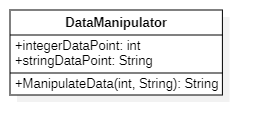
\includegraphics{ClassDiagramExample1}
    \caption{Yksittäisen luokan esittäminen UML-luokkakaaviossa}
    \label{luokkakaavioluokka}
    \setfloatalignment{b}
\end{listing}

\newthought{Luokkakaaviossa ohjelmiston} erilaisten luokkien esittäminen on kuitenkin vain pieni
osa kaavion käyttöä. Tärkein luokkakaavion käyttötarkoitus on luokkien välisten suhteiden
esittäminen ohjelmistossa. Luokkakaavio sisältää näiden suhteiden kuvaamiseen erilaisia
yhteystyyppiä, joita luokkien välille voidaan piirtää. Näistä käytetyimmät ovat yleistä
assosiaatiota, periytymistä, aggregaatiota ja kompositiota kuvaavat yhteydet. Yhteyden tarkka
tyyli riippuu kaavionpiirto-ohjelmasta. Yleensä assosiaatiota kuvaava yhteys on yksinkertainen
viiva luokkien välillä, periytymistä kuvaava yhteys on nuoli lapsiluokasta emoluokkaan ja
aggregaatiota ja kompositiota kuvaavat yhteydet ovat viivoja, jotka päättyvät vinoneliöön
omistussuhteen omistavan osapuolen päässä. Aggregaatiossa vinoneliö on täyttämätön,
kompositiossa täytetty. Seuraava kaavio esittelee kaikki neljä yhteystyyppiä.

\begin{listing}
    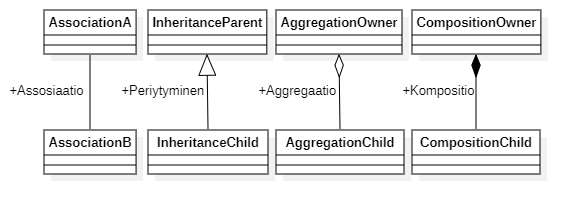
\includegraphics{ClassDiagramExample2}
    \caption{Luokkien välisten suhteiden esittäminen UML-luokkakaaviossa}
    \label{luokkakaavioluokka}
    \setfloatalignment{b}
\end{listing}

\subsection{Kaavioiden käyttö ohjelmiston suunnittelussa}
\label{UMLkäyttö}

\newthought{\gls{UML} kehitettiin} alun perin aikakaudella, jolloin vesiputousmallia pidettiin
erinomaisena vaihtoehtona ohjelmistoprojektin projektinhallintamalliksi ja ketterä kehitys oli
täysin tuntematon käsite. Tällöin ohjelmiston täydellisen rakenteen mallintamisen UML-kaavioilla 
ajateltiin olevan järkevä tapa suunnitella ohjelmistoja. Modernissa ohjelmistokehityksessä
vesiputousmalli on kuitenkin pudonnut pois suosiosta ja se on korvattu lähinnä ketterän kehityksen
innoittamilla projektinhallintametodeilla, kuten Scrum ja XP. Täten myös UML-kaavioiden rooli
osana ohjelmitonkehitysprosessia on modernisoitunut. Yleinen vallitseva käsitys alalla on, että
kaavioiden ei pitäisi olla yleisessä käytössä, vaan niitä kuuluisi käyttää vain nopeaan
ohjelmiston mallintamiseen erityisesti tehtäessä yhteistyötä usean kehittäjän kesken.

%%%%%%%%%%%%%%%%%%%%%%%%%%%%%%%%%%%%%%%%%%%%%%%%%%%%%%%%%%%%%%%%%%%%%%%%%%%%%%%%%%%%%%%%%%%%%%%%%%
% % % % % % % % % % % % % % % % % % % % % % % % % % % % % % % % % % % % % % % % % % % % % % % % %
%%%%%%%%%%%%%%%%%%%%%%%%%%%%%%%%%%%%%%%%%%%%%%%%%%%%%%%%%%%%%%%%%%%%%%%%%%%%%%%%%%%%%%%%%%%%%%%%%%

\chapter{Periytyminen ja Java}
\label{periytyminen2}

\newthought{\Gls{periytyminen} käsitteenä} käytiin läpi viime luvussa, mutta sen soveltaminen
käytännön ohjelmistotuotantoon jätettiin käsittelemättä. Tämän luvun tavoitteena on opettaa
periytymisen käyttö Javassa ja samalla syventyä periytymisen hyötyihin ja haittoihin, sen
oikeaoppisiin käyttökohteisiin ja teoriaan periytymisen takana.

%%%%%%%%%%%%%%%%%%%%%%%%%%%%%%%%%%%%%%%%%%%%%%%%%%%%%%%%%%%%%%%%%%%%%%%%%%%%%%%%%%%%%%%%%%%%%%%%%%

\section{Periytymisen perusteet ja extends}
\label{periytyminen3}

\subsection{Avainsana extends}
\label{extends}

\newthought{Javassa \gls{periytyminen}} toteutetaan \newjava{extends}-avainsanan avulla. Avainsana
sijoitetaan lapsiluokan määritelmään luokan nimen perään, niin että toivotun kantaluokan nimi
seuraa avainsanaa. Tämän jälkeen luokan määritelmää jatketaan normaalisti. Seuraava koodiesimerkki
esittelee yksinkertaisen periytymiseen pohjaavan rakenteen luomisen Javassa.

\code{week6/basicinheritanceexample}{Parent}{Periytymisesimerkin kantaluokka}
\code{week6/basicinheritanceexample}{Child}{Periytymisesimerkin lapsiluokka}
\code{week6/basicinheritanceexample}{BasicInheritanceExample}{Periytymisesimerkin pääluokka}

\subsection{Kantaluokan toiminnallisuuksien uudelleenmäärittely}
\label{overriding}

\newthought{Aina ei} ole toivottavaa, että lapsiluokka perii kaiken kantaluokan toiminnallisuuden.
Tätä varten Java tarjoaa mahdollisuuden uudelleenmääritellä periytettyjen luokkien perimiä
metodeja. Tämä metodin \neweng{korvaaminen}{overriding} tapahtuu yksinkertaisesti määrittelemällä
lapsiluokassa metodi, jonka \gls{signatuuri} on tismalleen sama, kuin kantaluokan korvattavan
metodin. Tällöin kutsuttaessa lapsiluokan metodia kyseisellä signatuurilla ajetaan lapsiluokassa
määritelty versio metodista. Seuraava koodiesimerkki esittelee metodin toiminnan korvaamisen
käytännössä.

\code{week6/overridingexample}{Parent}{Korvaamisesimerkin kantaluokka}
\code{week6/overridingexample}{Child}{Korvaamisesimerkin lapsiluokka}
\code{week6/overridingexample}{OverridingExample}{Korvaamisesimerkin pääluokka}

\subsection{Periytyminen ja tyypitys}
\label{casting2}

\newthought{Oppaan luvussa} \nameref{casting} kerrottiin Javan
\gls{pakotettu tyyppimuunnos}-operaatiosta, jolla jonkin tyypin muuttuja voidaan koittaa pakottaa
jonkin toisen tyypin muuttujaan. Luvussa annettiin esimerkki perustietotyyppien kohdalla, mutta
luokkiin kohdistuvat tapaukset jätettiin huomioimatta, koska niiden ymmärtäminen vaatii
perusymmärryksen periytymisen toiminnasta Javassa. Vaikka Java on vahvasti tyypitetty kieli, ei se
vaadi aina muuttujan ja muuttujaan tallennetun tiedon olevan yksi yhteen samaa tietotyyppiä:
minkä tahansa muuttujan arvoksi Javassa kelpaa paitsi muuttujan tietotyypin ilmentymä, myös mikä
tahansa tietotyypin lapsiluokan ilmentymä. Tässä tapauksessa Java suorittaa automaattisen
tyyppimuunnoksen lapsiluokasta kantaluokaksi viitatessaan lapsiluokan olioon: koska lapsiluokka
perii kantaluokan toiminnallisuudet, sisältää se aina vähintään samat kentät kuin kantaluokka.
Joskus ilmenee kuitenkin tarve käsitellä tällä tavalla säilöttyä lapsiluokan ilmentymää aidosti
oman luokkansa ilmentymänä. Tällöin voidaan suorittaa \gls{pakotettu tyyppimuunnos} luokasta
toiseen. Pakotettu tyyppimuunnos kahden luokan välillä onnistuu vain, jos luokka, joksi muuttuja
halutaan pakottaa, on periytetty muuttujan määritellystä luokasta.

\section{Periytyminen ja rakentajat}
\label{superprotected}

\subsection{Näkyvyysmääre protected}
\label{protected}

\newthought{Aiemmin oppaan} kappaleessa \nameref{näkyvyysmääreet} käytiin läpi käsite
\gls{nakyvyysmaare} ja avainsanat \java{public} ja \java{private}. Näiden ja oletusnäkyvyyden
lisäksi Javassa on olemassa neljäs näkyvyysmääreavainsana \newjava{protected}. Avainsana määrittää
muuttujan tai metodin olevan näkyvissä vain luokalle itselleen, sekä kaikille luokan periville
luokille. Näkyvyysmääreen \java{private} omaava muuttuja tai metodi ei siis näy edes luokan
periville luokille.

\subsection{Periytyminen, rakentajat ja super}
\label{super}

\newthought{Luotaessa lapsiluokan} ilmentymiä Javassa on aina kutsuttava kantaluokan rakentajaa.
Mikäli kummallekaan luokalle ei ole määritelty rakentajaa, kutsuu Java automaattisesti kantaluokan
oletusrakentajaa rakentaessaan lapsiluokan ilmentymää. Mikäli lapsiluokalla ei ole rakentajaa,
mutta kantaluokalle halutaan määrittää rakentaja, jota lapsiluokan rakennus käyttää, on tämän
rakentajan oltava parametritön.

\newthought{Mikäli lapsiluokalle} luodaan itse määritelty rakentaja, on rakentajan kutsuttava
ensimmäisenä komentona jotain emoluokan rakentajaa. Tämän ei tarvitse olla parametritön
oletusrakentaja vaan mikä tahansa rakentaja kelpaa.

\newthought{Päästäkseen käsiksi} kantaluokkansa kenttiin, kuten rakentajiin, voi lapsiluokka
käyttää \newjava{super}-avainsanaa. Avainsana toimii viittauksena kantaluokan ilmentymään, jonka
pohjalle lapsiluokka on luotu. Käyttämällä avainsanaa metodikutsuna päästään käsiksi kantaluokan
rakentajametodin eri ylikuormituksiin ja käyttämällä pistenotaatiota päästään käsiksi kantaluokan
muuttujiin ja metodeihin näkyvyysmääreiden salliessa. Seuraavat koodiesimerkit esittelevät
rakentajien käytön periytymisen yhteydessä, sekä avainsanat \java{super} ja \java{protected}

\code{week6/inheritancewithconstructors}{ParentWithoutConstructor}{Rakentajaton kantaluokka}
\code{week6/inheritancewithconstructors}{ChildOfConstructorless}{Rakentajattoman kantaluokan
lapsiluokka, jolle on määritelty rakentaja}
\code{week6/inheritancewithconstructors}{ParentWithConstructor}{Kantaluokka, jolla on rakentaja}
\code{week6/inheritancewithconstructors}{ChildOfConstructorParent}{Rakentajallisen kantaluokan
lapsiluokka, jolle on määritelty erillinen rakentaja}

%%%%%%%%%%%%%%%%%%%%%%%%%%%%%%%%%%%%%%%%%%%%%%%%%%%%%%%%%%%%%%%%%%%%%%%%%%%%%%%%%%%%%%%%%%%%%%%%%%

\section{Periytymisen oikeaoppinen käyttö}
\label{periytyminen4}

\newthought{Periytyminen on} monimutkainen rakenne joka tarjoaa ohjemoijalle voimakkaan työkalun.
Tätä työkalua on helppo käyttää väärin mikäli periytymistä lähdetään käyttämään kaikkialla ja
siitä yritetään tehdä ratkaisu joka ongelmaan. Periytymiselle on oma paikkansa ohjelmiston
suunnittelussa ja se ratkaisee jotkin ongelmat erinomaisesti, mutta on olemassa tiettyjä
lainalaisuuksia, jotka on pidettävä mielessä periytymistä hyödynnettäessä. Näin varmistetaan, että
ohjelmiston kehittäminen helpottuu periytymisrakenteiden vaikutuksesta, sen sijaan että
kehittämisprosessia monimutkaistettaisiin turhaan ilman selkeitä hyötyjä periytymisestä.

\subsection{Liskovin korvaavuusperiaate}
\label{LSP}

\newthought{Kuten kapppaleen} \nameref{super} koodiesimerkeissä nähtiin, voidaan lapsiluokan olio
tallentaa muuttujaan, jonka tyypiksi on määritelty emoluokan olio. Tällöin muuttujaan tallennettua
olioita voidaan kohdella kuin emoluokan oliota. Tämä käyttäytyminen mahdollistaa monia hyödyllisiä
toiminnallisuuksia, kuten monen eri lapsiluokan ilmentymien tallentamista samaan \java{ArrayList}-
ilmentymään, kunhan kyseinen \java{ArrayList}-ilmentymä on luotu viitaten kantaluokkaan, eikä
lapsiluokkaan.

\newthought{Kuitenkin tällainen} luokkien käyttäminen luo velvotteita lapsiluokkien suunnitteluun.
Jotta edellä kuvailtu käyttötapa sujuisi ongelmitta, kuuluu lapsiluokkien ja emoluokan toteuttaa
\neweng{Liskovin korvaavuusperiaate}{Liskov Substitution Principle - LSP}. Periaate on osa
viiden periaatteen muodostamaa \neweng{SOLID-periaatteet}{SOLID-principles} -ryhmää. Periaatteet
on suunniteltu helpottamaan laadukkaan oliopohjaisen koodin tuottamista ja loput periaatteet
käsitellään myöhemmin luvussa \nameref{solid}.

\newthought{\Gls{Liskovin korvaavuusperiaate}} määrittelee kantaluokan ja lapsiluokkien suhteen
seuraavasti: "Mikä tahansa emoluokan ilmentymä pitäisi olla korvattavassa millä tahansa 
lapsiluokan ilmentymällä ilman että ohjelman toiminta häiriintyy." Käytännössä tämä tarkoittaa,
että lapsiluokkien ei pitäisi ylikirjoittaa emoluokkien julkisia kenttiä niin että kentän
toiminnallisuus ulkoa tarkasteltaessa muuttuu. Esimerkiksi metodin ylikirjoittaminen
toimimattomalla tyngällä rikkoo täten Liskovin korvaavuusperiaatetta.

%%%%%%%%%%%%%%%%%%%%%%%%%%%%%%%%%%%%%%%%%%%%%%%%%%%%%%%%%%%%%%%%%%%%%%%%%%%%%%%%%%%%%%%%%%%%%%%%%%

\section{Periytymisen rakenteita}
\label{periytyminen5}

\newthought{Tähän mennessä} oppaassa on käsitelty vain suoraa periytymistä, jossa
\gls{kantaluokka} ja \gls{lapsiluokka} ovat molemmat normaaleja Javan luokkia. Periytyminen on
kuitenkin rakenne, jota käytetään monimutkaisten teollisten ohjelmien suunnittelussa ja täten
suurimpaan osaan oliopohjaisia kieliä on kehitetty rakenteita periytymiseen pohjaavan
arkkitehtuurin siistimiseen. Näistä tärkeimmät ovat \neweng{abstrakti luokka}{abstract class} ja
\neweng{rajapinta}{interface}. Tämä kappale käy läpi näiden rakenteiden käytön koodissa ja niiden
käyttötarkoitukset, sekä puhuu hieman rakenteiden eroista.

\subsection{Abstrakti luokka}
\label{abstract}

\newthought{\Gls{abstrakti luokka}} on oliopohjainen rakenne, jossa luokan määritelmästä tehdään
pelkkä muotti, jonka ainoa tehtävä on toimia pohjana kyseisestä luokasta periytyville
lapsiluokille. Tällaisen rakenteen tehtävänä on varmistaa että jokainen luokka, joka periytyy
abstraktista kantaluokasta toteuttaa jonkin jaetun toiminnallisuuden ja samalla estää kantaluokan
suora käyttäminen koodissa, koska sen ei kuulukaan tietää miten tämän toiminnallisuuden 
implementaatio tapahtuu. Luokasta tehdään abstrakti lisäämällä \newjava{abstract}-avainsana luokan
määritelmään \java{class}-avainsanan eteen. Abstraktin luokan ei-abstraktin lapsiluokan nimi on
\neweng{konkreettinen luokka}{concrete class}.

\newthought{Jokaisella abstraktilla} luokalla on oltava vähintään yksi 
\neweng{abstrakti metodi}{abstract method}. Tämä metodi määritellään luomalla metodi, joka
sisältää pelkän signatuurin ilman runkoa ja lisäämällä metodin määritelmään \java{abstract}
-avainsana näkyvyysmääreen jälkeen. Abstrakti metoodi on siis ikään kuin musta laatikko. Sen
argumentit ja paluuarvo tiedetään, mutta abstrakti kantaluokka, joka määrittelee metodin ei
kerro, miten metodeista saadaan paluuarvo vaan jokaisen konkreettisen lapsiluokan on
määriteltävä tämä itse.

\newthought{Abstraktin luokan} käyttö koodissa vaatii yleensä jonkin jaetun toiminnallisuuden
tarpeen toteamista ja tämän toiminnallisuuden eristämistä abstraktiin luokkaan. Seuraava
koodiesimerkki esittelee abstraktin kantaluokan ja konkreettisen lapsiluokan luomisen. Esimerkissä
luodaan "AbstractLogger"-kantaluokka, joka sisältää \java{protected}-metodin "formatLogString" ja
abstraktin julkisen metodin "logString". Sen jälkeen kantaluokasta tehdään konkreettinen
lapsiluokka "CommandLineLogger", joka sisältää määritelmän kantaluokan "logString"-metodille.
Huomaa, kuinka lapsiluokka pystyy käyttämään "formatLogString"-metodia, joka on määritelty
kantaluokassa.

\code{week6/abstractexample}{AbstractLogger}{Abstrakti loggaajapohja}
\code{week6/abstractexample}{CommandLineLogger}{Loggaajaan konkreettinen implementaatio, joka
tulostaa saadun tekstidatan komentoriville}

\subsection{Rajapinta}
\label{interface}

\newthought{Toinen tapa} eristää luokkien jakamaa toiminnallisuuttaa koodissa on rajapintaluokka,
joka luodaan \java{interface}-avainsanalla. Rajapintaluokan tehtävä on luokan nimen mukaisesti
määrittää jokin \gls{rajapinta} jonka muut ohjelmiston luokat voivat sitten ilmoittaa täyttävänsä.
Toisin kuin \gls{abstrakti luokka}, rajapintaluokka voi sisältää ainoastaa julkisia ja staattisia 
vakiotietokenttiä, eikä rajapintaluokkaa voi käytää kantaluokkana periytymisessä. Tämän sijaan
mikä tahansa ohjelmiston luokka voi ilmoittaa, että se \neweng{toteuttaa}{implement}
rajapintaluokan. Luokan, joka toteuttaa rajapintaluokan on määriteltävä jokainen rajapinnassa
määritelty metodi. Näistä määritelmistä jokaisella pitää olla identtinen \gls{signatuuri}
rajapintaluokan vastaavan metodin määritelmän kanssa.

\newthought{Rajapintaluokka määritellään} Javassa korvaamalla normaalin luokan määritelmän 
\java{class}-avainsana \newjava{interface}-avainsanalla. Rajapintaluokkasta ei voi luoda
ilmentymiä, eikä luokalle voi määrittää rakentajaa. Ainoat tietokentät, jotka ovat hyväksyttyjä
rajapintaluokassa ovat oletuksena näkyvyydeltään julkisia luokkamuuttujavakioita. Mikäli muuttujan
määritelmä rajapintaluokassa ei sisällä avainsanoja \java{public}, \java{static} ja \java{final}
lisätään ne määritelmään automaattisesti. Muiden näkyvyysmääreiden käyttäminen estää ohjelmiston
rakentamisen.

\newthought{Rajapintaluokan kaikki} metodit ovat automaattisesti abstrakteja metodeja. Myös
metodien on oltava rajapintaluokassa julkisia muuttujien tapaan. Java tukee metodin
oletustoiminnallisuuden määrittelemistä \newjava{default}-avainsanalla, mutta mikäli ohjelmiston
kehitysvaiheessa huomataan tälle olevan tarvetta kannattaa miettiä tarkkaan, käytetäänkö
rajapintaluokkaa oikein; Avainsana on olemassa lähinnä mahdollistamaan myöhemmät laajennukset
yleisesti käytettyihin rajapintoihin eikä siihen kannata tukeutua. Tästä syystä oppaassa ei
myöskään käydä avainsanan käyttöä tämän tarkemmin läpi.

\newthought{Seuraava koodiesimerkki} esittelee simppelin "TextProvider"-rajapinnan luomisen ja
kyseisen rajapintaluokan implementoimisen konkreettiseen luokkaan.

\code{week6/interfaceexample}{TextProvider}{TextProvider rajapintaluokka}
\code{week6/interfaceexample}{FunctionalClass}{Luokka, joka implementoi TextProvider-rajapinnan}

\subsection{Rajapinta vai abstrakti luokka?}
\label{interface v abstract}

\newthought{Rajapintaluokka ja} abstrakti luokka muistuttavat toisiaan toiminnallisuuksiltaan ja
osin käyttötavoiltaankin. Niille molemmille löytyvät kuitenkin omat erilliset käyttökohteensa ja
syvempi ymmärrys luokkatyyppien toiminnallisuuksien eroista auttaa käsittämään nämä erilaiset
käyttökohteet.

\newthought{Koska luokkien} \neweng{moniperinta}{multiple inheritance} ei ole tuettua Javassa, ei
abstrakteja luokkia voi käyttää lisäämään yhdelle luokalle useamman eri luokan toiminnallisuuksia.
Tällainen on rajapintaluokkien tehtävä. Sen sijaan abstrakti luokka voi määritellä valmiiksi
toiminnallisuuksia ja datakenttiä itselleen, helpottaen lapsiluokkien kirjoittamista. Abstraktin
luokan pääkäyttötarkoitus onkin luoda koodiin jokin palvelu, kuten edellä sivuttu logien	
kirjoittaminen, jonka yleinen toiminnallisuus on tiedossa, mutta toteutus riippuu käytettävästä
kirjastosta. Esimerkiksi tässä logiesimerkissä, voitaisiin luoda abstrakti luokka, jolle
implementoidaan valmiiksi funktiot logien muotoiluun, mutta jonka loginkirjoitusfunktiot
määritellään abstrakteina, jolloin kutakin logikirjastoa käyttävä abstraktin luokan implementaatio
määrittelee kirjastoon nojaavan rajapintansa itse.

\newthought{Rajapintaluokkien tehtävä} puolestaan on yleensä luoda pieniä, selkeitä
toiminnallisuussopimuksia koodissa. Mikäli myöhemmin ilmenee tarve lisätä johonkin luokkaan jo
valmiiksi määritellyn rajapinnan toiminnallisuudet, voidaan luokan määritelmään lisätä tämä
rajapinta \java{implements}-avainsanalla. Esimerkiksi pelinkehityksessä saatetaan tarvita
tuhoutuvia objekteja, joita varten voitaisiin luoda "Destructable"-rajapintaluokka jolle on
määritelty "destroyObject"-metodi. Koodi voi sitten tarkistaa implementoiko jokin luokka tämä
rajapinnan \newjava{instanceof}-avainsanalla ja jos luokka implementoi "Destructable"-rajapinnan,
koodi voi kutsua "destroyObject"-metodia luokan ilmentymästä tuhoten objektin.

\newthought{Rajapintaluokan ja} abstraktin luokan käyttötarkoitukset siis eroavat toisistaan
hieman. Yleisesti rajapintaluokan tehtävä on määrittää laajemmin käytössä oleva sopimus, joka
voidaan implementoida eri kohdissa koodia eri luokille. Tästä hyvä esimerkki on
\nameref{serialisaatio}-kappaleessa käsiteltävä \java{Serializable}-rajapintaluokka. Abstrakti
luokka taas määrittää yhden toiminnallisuudeltaan rajatun luokkatyypin, mutta antaa tämän
toiminnallisuuden toteutusvastuun eteenpäin kantaluokan lapsiluokille. Mahtava esimerkki tästä
ovat Minecraft-pelin kuutiot. Jokainen kuutiotyyppi on abstraktin "Block"-luokan konkreettinen
lapsiluokka, joka määrittää yksittäisen kuutiotyypin tarkemmat toiminnallisuudet.

\newthought{Oppaan koodiesimerkeissä} tämä käyttötapojen ero näkyy kappaleissa \nameref{abstract}
ja \nameref{interface}. Abstraktin luokan esimerkissä hyödynnetään abstraktin kantaluokan kykyä
määritellä konkreettisia metodeja kantaluokkaan: oletettavasti kaikki lapsiluokat hyödyntävät
"formatLogString"-metodia. Rajapintaluokkaesimerkissä puolestaan luotu "TextProvider"-rajapinta
on vain yksinkertainen rajapinta, jonka mikä tahansa ohjelmiston luokka saattaa toteuttaa
tarvittaessa. Abstraktilla luokalla on yksi suunniteltu käyttötarkoitus, jonka toteutustapa
määritellään lapsiluokan implementaatiossa, kun taas rajapintaluokan käyttötarkoitus ei ole niin
tarkkaan rajattu ja rajapintaa voidaan implementoida useammassa paikassa koodissa.

%%%%%%%%%%%%%%%%%%%%%%%%%%%%%%%%%%%%%%%%%%%%%%%%%%%%%%%%%%%%%%%%%%%%%%%%%%%%%%%%%%%%%%%%%%%%%%%%%%

\section{Serialisaatio}
\label{serialisaatio}

\newthought{Javassa ohjelmiston} omistama data on yleensä tallennettu oliomuodossa, mutta olion
tallentaminen tiedostoon tekstidatana ei ole erityisen helppoa. Se vaatisi kaikkien olion kenttien
muuttamista tekstiksi manuaalisesti aina oliota tallennettaessa ja tekstimuotoisen datan lukemista
ja uuden olion rakentamista luetusta tekstidatasta aina oliota ladattaessa. Tähän tarkoitukseen
Javasta löytyy erikseen \gls{serialisaatio}-niminen tekniikka, joka mahdollistaa olioiden
automaattisen muuttamisen tallennettavaan muotoon ja tämän muodon muuttamisen takaisin olioksi.

\newthought{Serialisaatio on} mahdollista vain luokille, jotka implementoivat
\newjava{Serializable}-rajapinnan. Tämän lisäksi kaikkien luokan muuttujien on myös oltava
tietotyyppiä, joka implementoi tämän rajapinnan. Suurimmaksi osaksi tämä koskee vain käyttäjän
määrittelemiä luokkia, sillä kaikki perustietotyypit ja suurin osa standardikirjaston yleisesti
käytetyistä luokista, kuten kokoelmat, implementoivat \java{Serializable}-rajapinnan.

\newthought{Jos luokka} ja kaikki luokan muuttujat implementoivat \java{Serializable}-rajapinnan,
voidaan luokan ilmentymä muuttaa tekstimuotoon \newjava{ObjectOutputStream}-luokan avulla.
Luokan julkinen rakentaja ottaa \java{OutputStream}-olion, joka edustaa datakuluttajaa, johon
serialisoitava objekti kirjoitetaan. Luodusta ilmentymästä voidaan kutsua ilmentymän writeObject-
metodia serialisoitavalla oliolla. Tämä kirjoitaa olion serialisoidun tavudataversion
\java{ObjectOutputStream}-rakentajassa määriteltyyn \java{OutputStream}-olioon.

\newthought{Luokan deserialisaatio} tapahtuu \newjava{ObjectInputStream}-luokan avulla. Luokan
julkinen rakentaja ottaa \java{InputStream}-olion, joka edustaa datasyötettä, josta
deserialisoitava objekti on luettavissa. Luodusta ilmentymästä voidaan kutsua ilmentymän
readObject-metodia ilman argumentteja. Tämä palauttaa deserialisoidun olion luetun tavudatan
pohjalta.

\newthought{Seuraava koodiesimerkki} esittelee serialisoitavan luokan luomisen, serialisaation
tiedostoon ja deserialisaation tiedostosta. Huomioi, että mikäli serialisoituja olioita
tallennetaan tiedostoon, on normaalia nimetä tiedosto ".ser"-päätteellä.

\code{week6/serializationexample}{SerializableData}{Serialisoitava luokka}
\code{week6/serializationexample}{SerializationExample}{Serialisaatioesimerkin pääluokka}

%%%%%%%%%%%%%%%%%%%%%%%%%%%%%%%%%%%%%%%%%%%%%%%%%%%%%%%%%%%%%%%%%%%%%%%%%%%%%%%%%%%%%%%%%%%%%%%%%%
% % % % % % % % % % % % % % % % % % % % % % % % % % % % % % % % % % % % % % % % % % % % % % % % %
%%%%%%%%%%%%%%%%%%%%%%%%%%%%%%%%%%%%%%%%%%%%%%%%%%%%%%%%%%%%%%%%%%%%%%%%%%%%%%%%%%%%%%%%%%%%%%%%%%

\addtocounter{chapter}{1}
\chapter{Singleton-suunnittelumalli}
\label{singletonkappale}

\newthought{Välillä ohjelmistoa} luodessa on tarve luoda luokka, josta on olemassa vain yksi
\gls{ilmentyma}, jota muu ohjelma voi kutsua tarvittaessa. Tähän käyttötarkoitukseen on kehitettu
suunnittelumalli nimeltä \neweng{singleton}{singleton}. Suunnittelumallin ideana on tallentaa
luokan ilmentymä yksityiseen luokkamuuttujaan ja tarjota julkinen "getInstance"-luokkametodi,
joka joko hakee olemassaolevan ilmentymän luokkamuuttujasta tai luo uuden ilmentymän
luokkamuuttujaan, mikäli ilmentymää ei vielä ole olemassa. Seuraava koodiesimerkki esittelee
tämän toteutuksen käytännössä.

\code{week8}{SingletonExample}{Singleton-suunnittelumallin toteuttava luokka}

\newthought{\Gls{singleton}-suunnittelumallia} on kritisoitu, sillä se luo ohjelmistolle jaetun
julkisen tilan toimien käytännössä glorifioituna globaalina muuttujana. Mallille on kuitenkin
olemassa selkeitä hyödyllisiä käyttökohteita, kuten tietokantayhteyden standardointi. Nämä
käyttökohteet ovat yleensä jaettuja palveluita, jotka ovat joko lähes tai täysin tilattomia.
Vahvasti tilallisen olion tallentaminen singleton-luokkaan on valtava virheriski, koska olioon
pääse käsiksi mistä tahansa koodissa ja siten sen tila on erittäin helppo muuttaa epähuomiossa
virheelliseksi.

%%%%%%%%%%%%%%%%%%%%%%%%%%%%%%%%%%%%%%%%%%%%%%%%%%%%%%%%%%%%%%%%%%%%%%%%%%%%%%%%%%%%%%%%%%%%%%%%%%
% % % % % % % % % % % % % % % % % % % % % % % % % % % % % % % % % % % % % % % % % % % % % % % % %
%%%%%%%%%%%%%%%%%%%%%%%%%%%%%%%%%%%%%%%%%%%%%%%%%%%%%%%%%%%%%%%%%%%%%%%%%%%%%%%%%%%%%%%%%%%%%%%%%%

\chapter{SOLID-periaatteet, käyttäjän määrittelemät virheluokat}
\label{solid+exceptions}

%%%%%%%%%%%%%%%%%%%%%%%%%%%%%%%%%%%%%%%%%%%%%%%%%%%%%%%%%%%%%%%%%%%%%%%%%%%%%%%%%%%%%%%%%%%%%%%%%

\section{SOLID-periaatteet}
\label{solid}

\newthought{Tässä vaiheessa} opasta oppaan käyttäjä osaa jo toivottavasti tuottaa toimivaa
oliopohjaista koodia. Ikävä kyllä toimiva koodi ei tarkoita suoraan laadukasta koodia. Laadukas
koodi on uusiokäytettävää, helppolukuista ja laajennettavaa. Yksi laadukkaan koodin tuottamista
helpottamaan kehitetty menetelmä ovat \neweng{SOLID-periaatteet}{SOLID-principles}. Periaatteet
eivät ole kiveen hakattuja, mutta niiden noudattaminen tuottaa yleensä vähintään kohtalaisen
laadukasta koodia. Periaatteita on viisi: \neweng{yhden vastuun periaate}{Single Responsibility
Principle}, \neweng{avoin/suljettu-periaate}{Open Closed Principle}, aiemmin käsitelty
\gls{Liskovin korvaavuusperiaate} (kappale \nameref{LSP}), \neweng{rajapintojen erottelu
-periaate}{Interface Segregation Principle} ja \neweng{kaanteisten riippuvuuksien periaate}
{Dependency Inversion Principle}. SOLID-lyhenne syntyy periaatteiden englanninkielisten nimien
ensimmäisistä kirjaimista. Periaatteiden seuraaminen ei ole pakollista, mutta se yleensä helpottaa
koko ohjelmointiprosessia pidemmällä aikavälillä.

\subsection{Yhden vastuun periaate}
\label{SRP}

\newthought{Ensimmäinen periaate} on \gls{yhden vastuun periaate}. Se käsittelee luokkien
suunnittelua ja käyttöä. Periaatteen mukaan jokaisella luokalla pitäisi olla yksi, ja vain yksi
vastuu. Mikäli luokan käyttötarkoitus ei ole kuvailtavissa yhdellä melko yksinkertaisella
lauseella, rikkoo luokka todennäköisesti yhden vastuun periaatetta.

\subsection{Avoin/suljettu-periaate}
\label{OCP}

\newthought{Toinen SOLID-periaate} on \gls{avoin/suljettu-periaate}. Sen mukaan ohjelmiston
koodin tulisi olla avoin laajennuksille, mutta suljettu muutoksille. Käytännössä tämä tarkoittaa,
että toteutettujen toiminnallisuuksien koodin tulisi olla suunniteltu olettaen, että sama koodi
säilyy ohjelmistossa koko sen elinkaaren läpi. Toisaalta taas koodin tulisi olla helposti
laajennettavissa. Periaatteen tavoitteena on rohkaista suunnittelemaan ohjelmistoja niin, että
ensisijainen tapa lisätä toiminnallisuuksia ei olisi vanhojen luokkien muokkaaminen, vaan uusien
lisääminen.

\newthought{Normaalisti esimerkiksi} \java{switch}-rakenteiden käyttö monesti rikkoo 
avoin/suljettu periaatetta. Mikäli rakenteeseen tarvitsee lisätä uusi haara, täytyy ohjelmoijan
käydä muokkaamassa vanhaa koodia, mikä altistaa ohjelmiston virhetiloille, kun kertaalleen
toimivaksi todettua koodia muokataan myöhemmin. Oliopohjaisessa ohjelmoinnissa kannustetaan
korvaamaan switch rakenteet \neweng{strategia}{strategy}-suunnittelumallilla. Seuraava
koodiesimerkki havainnollistaa saman rakenteen toteuttamisen enum-switch yhdistelmällä, ja
strategia-suunnittelumallilla. Huomaa, kuinka paljon helpompaa jälkimmäisen laajentaminen on,
rakenteen sisäistä koodia ei tarvitse muuttaa ollenkaan, vaikka esimerkkiin lisättäisiin
väli-ilmansuunnat tai muita suuntia. Jokainen suuntaluokka voisi määritellä hahmon liikkeen
omassa movePlayer-metodissaan. Sen sijaan ensimmäisen esimerkin laajentaminen vaatii jo valmiin
koodin muokkaamista aina, kun rakenteeseen halutaan lisätä uusi suunta.

\code{week9/openclosedexample}{Player}{Pelaaja-luokka, jonka koordinaatteja esimerkissä pyritään
muuttamaan}
\code{week3/enumexample}{CompassPoint}{Ilmansuunnat \java{enum}-luokalla esiteltynä}
\code{week9/openclosedexample}{MoveSwitch}{Hahmon liikuttaminen \java{switch}-rakenteella ja
ilmansuuntia esittävällä \java{enum}-rakenteella}
\code{week9/openclosedexample}{MovementCommand}{Rajapintaluokka hahmon liikkuttamiseen
\gls{strategia}-suunnittelumallilla}
\code{week9/openclosedexample}{MoveNorth}{Liikkumiskomento pohjoiseen}
\code{week9/openclosedexample}{MoveEast}{Liikkumiskomento itään}
\code{week9/openclosedexample}{MoveSouth}{Liikkumiskomento etelään}
\code{week9/openclosedexample}{MoveWest}{Liikkumiskomento länteen}
\code{week9/openclosedexample}{MoveStrategy}{Hahmon liikuttaminen 
\gls{strategia}-suunnittelumallilla}

\subsection{Rajapintojen erottelu -periaate}
\label{ISP}

\newthought{SOLID-periaatteista} neljäs on \gls{rajapintojen erottelu -periaate}. Se käsittelee
rajapintaluokkien käyttöä ja luokkien kokoa. Periaatteen mukaan, jos luokka implementoi
rajapintaluokan, täytyisi luokan tarvita kaikkia rajapinnan metodeja. Rajapintaluokkien pitäisi
olla siis tarpeeksi hyvin rajattuja, jotta niiden kaikki metodit kuuluvat yhteen
toiminnallisuuspakettiin. Periaate kannustaa täten luomaan monta pientä rajapintaa ja
implementoimaan niistä tarvittavat yhden valtavan rajapinnan sijaan. Tämä helpottaa jo luotujen
rajapintaluokkien uudelleenkäyttöä.

\subsection{Käänteisten riippuvuuksien periaate}
\label{DIP}

\newthought{Viimeinen SOLID-periaate} on \gls{kaanteisten riippuvuuksien periaate}. Se
käsittelee riippuvuuksien suuntaa ohjelmistossa. Periaate perustuu toiveeseen korkean
abstraktiotason komponenttien helposta uusiokäytöstä ja niiden vastustuskyvystä muutoksille.
Molemmat ominaisuudet vaativat, että kyseiset komponentit eivät ole suoraan riippuvaisia
käyttämistään alemman tason komponenteista. Periaate on yleensä esitetty kahtena perusideana:

\begin{enumerate}
	\item Korkean tason komponenttien ei pitäisi olla riippuvaisia matalan tason komponenteista. Molempien pitäisi olla riippuvaisia abstraktioista.
	\item Abstraktioiden ei pitäisi olla riippuvaisia yksityiskohdista. Yksityiskohtien pitäisi olla riippuvaisia abstraktioista.
\end{enumerate}

\newthought{Käytännössä tämä} tarkoittaa, että seuratakseen käänteisten riippuvuuksien periaatetta
korkean tason luokka ei saa luoda itse tarvitsemiaan alemman tason riippuvuuksia, vaan sen on
pyydettävä ne muulta ohjelmistolta rakentajassaan. Täten täytetään ensimmäisen säännön ensimmäinen
puoli. Säännön toinen puoli puolestaan täyttyy, kun korkean tason komponentti ei pyydä
rakentajassaan konkreettista luokkaa riippuvuutena, vaan rajapintaluokkaa, jonka alemman tason
komponentti toteuttaa. Seuraava kuvapari havainnollistaa tämän suorat riippuvuudet rikkovan
arkkitehtuurin \gls{UML}-luokkakaaviona. Huomaa HighLevelService-luokan assosiaationuolen tyypin
muuttuminen. Ensimmäisessä kuvassa luokkien välinen suhde on \gls{kompositio}, kun taas toisessa
suhteen tyyppi on \gls{aggregaatio}. Tämä johtuu teoreettisesta LowLevelServiceInterface-luokan
vastaanottamisesta luokan rakentajassa konkreettisen LowLevelService luokan luonnin sijaan.
Täten LowLevelServiceInterface luokan elinikä ei enää ole sidottu HighLevelService-luokan
elinikään.

\begin{listing}
    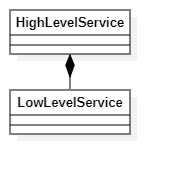
\includegraphics{NoDIPExample}
    \caption{Luokkakaavio suorasta riippuvuudesta korkean ja matalan tason luokan välillä}
    \label{luokkakaavioluokka}
    \setfloatalignment{b}
\end{listing}

\begin{listing}
    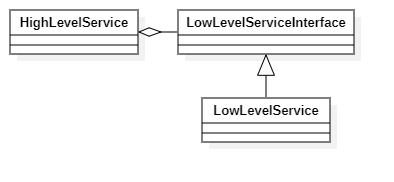
\includegraphics{DIPExample}
    \caption{Luokkakaavio rajapintaluokalla piilotetusta riippuvuudesta korkean ja matalan tason luokan välillä}
    \label{luokkakaavioluokka}
    \setfloatalignment{b}
\end{listing}

\newthought{Käänteisten riippuvuuksien} periaatteeseen sitoutuminen tuottaa yleensä jonkin verran
ylimääräistä koodia riippuvuuskohtien rajapintojen luonnissa. Lisäksi ohjelmistoon on luotava
luokka tai luokkia, joiden vastuulla on ohjelmiston riippuvuuksien rakentaminen käynnistyksen
yhteydessä, koska korkean tason luokat eivät enää osaa itse rakentaa tarvitsemiaan matalan tason
palveluita. Periaate saattaa vaikuttaa turhalta teoreettiselta näpertelyltä ja sitä se
todennäköisesti onkin pienemmissä projekteissa. Periaatteella on kuitenkin valtava jalansija
teollisessa koodintuotannossa, eikä tämä ole sattumaa. Käänteisten riippuvuuksien periaatetta
noudattavaa koodia on uskomattoman helppo testata, koska jokainen palvelu voidaan irrottaa lopun
ohjelmiston kontekstista ja palvelua voidaan testata puhtaasti oman toiminnallisuutensa suhteen.
Opas ei siis suosittele kaikkia oppaan lukijoita toteuttamaan omia projektejaan käänneteisten
riippuvuuksien periaatteen mukaan. Periaate kannattaa kuitenkin opetella, sillä siirryttäessä
työelämään sekä koodikantojen koko että testaamisen merkitys moninkertaistuvat ja silloin
käänteisten riippuvuuksien periaate kohoaa todennäköisesti tärkeimmäksi kaikista 
SOLID-periaatteista.

%%%%%%%%%%%%%%%%%%%%%%%%%%%%%%%%%%%%%%%%%%%%%%%%%%%%%%%%%%%%%%%%%%%%%%%%%%%%%%%%%%%%%%%%%%%%%%%%%%

\section{Käyttäjän määrittelemät virhetilat}
\label{exception}

\newthought{Aiemmin oppaan} luvussa \nameref{try-catch} käytiin läpi Javan
virhetilanhallintasyntaksi. Luvussa käsiteltiin standardikirjaston toimintojen aiheuttamia
virhetiloja, mutta standardikirjasto ei omista yksinoikeutta virhetilojen aiheuttamiseen. Käyttäjä
voi myös itse nostaa ja jopa luoda uusia virhetilaluokkia. Virhetilaluokka nostetaan
\newjava{throw}-avainsanalla ja käyttäjä voi luoda omia virhetilaluokkiaan periyttämällä luokan
\newjava{Exception}-luokasta.

\subsection{Käyttäjän määrittelemä virhetilaluokka}
\label{exception}

\newthought{Ohjelmistolla voi} olla monia syitä käyttää käyttäjän itse määrittelemiä virhetiloja.
Perimmäinen syy virhetilalle on aina mahdollistaa jostakin ajonaikaisesta ongelmasta toipuminen.
Java tarjoaa virhetilaluokat laitteiston ja standardikirjaston toiminnasta riippuville ongelmille,
mutta se ei pysty tarjoamaan ohjelmiston suunnittelusta aiheutuville mahdollisille ongelmille
erikseen määriteltyjä virheitä. Esimerkiksi virheellinen käyttäjäsyöte voi aiheuttaa tilanteen,
jossa ohjelman ajoa ei voida jatkaa normaalisti. Tätä varten Java tarjoaa käyttäjälle
mahdollisuuden luoda omia virhetilaluokkiaan. Tämä tapahtuu yksinkertaisesti periyttämällä
toivotun virhetilaluokan \java{Exception}-luokasta.

\subsection{Manuaalinen virhetilan aiheuttaminen}
\label{throws}

\newthought{Oman virhetilaluokan} luominen ei hyödytä ohjelmistoa, ellei ohjelmointikieli tarjoa
työkaluja käyttää luotua virhetilaluokkaa. Tätä varten Java tarjoaa \java{throw}-avainsanan.
Avainsanaa käytetään lisäämällä avainsanan perään jonkin virhetilan ilmentymä, tai luomalla uusi
virhetilaluokan ilmentymä \java{new}-avainsanalla. Tämä aiheuttaa koodin siirtymisen
virhetilanhallintaan, josta aiheutettu virhetila voidaan hallitusti napata ylemmällä tasolla. Tämä
mahdollistaa siistin virhetilasta palautumisen tasolla, jossa se on mahdollista. 

\newthought{Pelkkä virhetilan} nosto ei kuitenkaan riitä, mikäli virhetilan palautuminen ei
tapahdu saman metodin sisällä. Java vaatii käyttäjää määrittelemään metodit, jotka voivat
aiheuttaa käsittelemättömiä virhetiloja \newjava{throws}-avainsanalla. Avainsana lisätään metodin
määritelmään nimen ja parametrien jälkeen ja avainsanan perään lisätään virhetilaluokka tai 
-luokat, joita metodi saattaa aiheuttaa. Javan kääntäjä vaatii käyttäjää käsittelemään kaikki
virhetilat jota kutsuttu metodi voi aiheuttaa. Tämän vaatimuksen voi kiertää määrittelemällä
metodin, joka kutsuu virhetilan aiheuttavaa metodia, myös kyseisen virhetilan aiheuttavaksi. Tämä
siirtää vastuun virhetilan käsittelystä yhtä kooditasoa ylemmäksi. Yleensä virhetilat kannattaa
kuitenkin käsitellä alimmalla tasolla, jolla puhdas palautuminen virhetilasta on mahdollista.

\newthought{Seuraava koodiesimerkki} esittelee käyttäjän määrittelemän virhetilaluokan luomisen,
sekä virhetilan aiheuttavan metodin määrittelemisen. Virhetila johtuu käyttäjän virheellisestä
syötteestä, joten se käsitellään alimalla tasolla, jolla täydellinen toipuminen on mahdollista:
käyttäjärajapinnassa.

\code{week9/exceptionexample}{NoDatabaseEntryException}{Itse määritelty virhetilaluokka}
\code{week9/exceptionexample}{DatabaseConnection}{Yksinkertaistettu tietokantayhteyttä matkiva
luokka, joka nostaa luodun virhetilan jos annettua esinettä ei löydy}
\code{week9/exceptionexample}{ExceptionExample}{Pääluokka, joka kutsuu luotua valetietokantaa}

%%%%%%%%%%%%%%%%%%%%%%%%%%%%%%%%%%%%%%%%%%%%%%%%%%%%%%%%%%%%%%%%%%%%%%%%%%%%%%%%%%%%%%%%%%%%%%%%%%
% % % % % % % % % % % % % % % % % % % % % % % % % % % % % % % % % % % % % % % % % % % % % % % % %
%%%%%%%%%%%%%%%%%%%%%%%%%%%%%%%%%%%%%%%%%%%%%%%%%%%%%%%%%%%%%%%%%%%%%%%%%%%%%%%%%%%%%%%%%%%%%%%%%%

\chapter{Geneerisyys ja iteraattorit}
\label{generic+iterator}

\section{Geneerisyys}
\label{generic}

\newthought{Geneerisyys on} suunniteltu mahdollistamaan laajempi uudelleenkäyttö luokille ja
metodeille. Esimerkiksi ilman geneerisyyttä kaikista kokoelmatyypeistä pitäisi olla erillinen
versio jokaikiselle luokalle, jota kokoelmassa säilötään. Oppaassa on sivuttu jo geneerisyyttä
kappaleessa \nameref{kokoelmista}, mutta konsepti on monimutkainen, joten tarkempi käsittely
jätettiin silloin välistä. Tämä kappale antaa yleiskatsauksen tähän hyödylliseen, mutta
monimutkaiseen Javan ominaisuuteen.

\subsection{Geneerisyyden perusteet}
\label{genericBasics}

\newthought{Oppaan kappaleessa} \nameref{listat} mainittiin käsite \gls{geneerinen luokka}. 
Geneerinen luokka ja \neweng{geneerinen metodi}{generic method} ovat yleisiä käsitteitä
staattisesti tyypitetyille kielille ja viittaavat luokkaan ja metodiin, jotka määritellään
suhteessa johonkin toiseen luokkaan. Tämä geneerinen \neweng{tyyppiparametri}{type paremeter}
kirjoitetaan yleensä luokan määritelmän yhteydessä yhdellä kirjaimella, joka on toivottua
parametria kuvaavan sanan ensimmäinen kirjain; T - Type, E - Element, K -Key, N - Number, V -
Value. Monta tyyppiparametria omaavassa luokassa voidaan käyttää joko kirjaimia S, U, V, jne. tai
numeroida parametrit (T1, T2, jne.). Tyyppiparametri sijaitsee luokan määritelmässä luokan nimen
perässä ja metodin määritelmässä metodin paluuarvotyypin edellä. Molemmissa tapauksissa
tyyppiparametri suljetaan pienempi kuin- ja suurempi kuin -merkkien väliin. Mikäli luokka tai
metodi on riippuvainen useammasta tyypistä annetaan kaikki tyypit samojen merkkien välissä,
pilkulla eroteltuina, metodin parametrien tapaan. 

\newthought{\Gls{tyyppiparametri} voi} olla rajoitettu perintäehdolla, jolloin kaikkien
geneeristä luokkaa tai metodia kutsuvien koodin osien on toteutettava tämä ehto luokalle tai
metodille tarjoamissaan tyypeissä. Tämä tapahtuu lisäämällä heti rajattavan tyyppiparametrin
perään \java{extends}-avainsana ja ylärajaluokka. Rajattu tyyppiparametri vaatii, että parametriin
annettu tyyppi on joko ylärajaluokan ilmentymä tai jonkin ylärajaluokasta periytyvän luokan
ilmentymä.

\newthought{Kuten kappaleessa} \nameref{listat} opittiin, määriteltäessä geneerisen luokan
ilmentymän säilövää muuttujaa täytyy tyyppiparametri antaa samalla notaatiolla kuin luokan
määritelmässä. Tätä geneerisen luokan tyyppiparametrin määrittelemistä kutsutaan
parametrisoinniksi. Luotaessa ilmentymää olemassa olevaan parametrisoituun muuttujaan, voidaan
Java 7:ssä ja uudemmissa Javan versioissa jättää tyyppiparametrit määrittelemättä: kääntäjä osaa
tulkita ne muuttujasta, johon ilmentymää luodaan. Samaan tapaan kutsuttaessa geneeristä metodia
kääntäjä tulkitsee tyyppiparametrit annettujen muuttujien tyypeistä.

Seuraava koodiesimerkki esittelee
geneerisen säilöluokan toteuttamisen ja geneerisen metodin toteuttamisen säilöluokalle, sekä
luokan ilmentymän luomisen ja metodin kutsumisen.

\code{week10/genericexample}{GenericContainer}{Geneerinen säiliöluokka, jolla on geneerinen metodi
säiliön sisällön vaihtamiseen}
\code{week10/genericexample}{GenericExample}{Säiliöluokan ilmentymän luominen, ja vaihtometodin
kutsuminen}

\subsection{Geneerisyys ja perintä}
\label{genericInheritance}

\newthought{Tyyppiparametrin konkreettinen} määrittäminen on mahdollista myös perinnän yhteydessä.
Generisestä kantaluokasta on mahdollisuus luoda parametrisoitu lapsiluokka ja geneerisestä
rajapintaluokasta on mahdollista luoda parametrisoitu implementaatio. Tällöin luotu luokka
ei enää ole geneerinen, sillä sen tyyppiparametria ei voida määrittää luokkaa luotaessa. Tätä
parametrisointia ei ole pakko toteuttaa, periytymisessä voidaan geneerinen parametri myös
jättää ennalleen tai sen rajausta voidaan tiukentaa. Rajauksen löysentäminen ei kuitenkaan ole
mahdollista. Mikäli kantaluokka on geneerinen tyypin T yli ja T on rajattu olemaan tietyn luokan
tai sen lapsiluokkien ilmentymä, ei voida ilmoitta T:hen käyvän minkä tahansa olion. Tämä rikkoisi
kantaluokan toiminnallisuuden ja täten ei seuraa \gls{Liskovin korvaavuusperiaate}tta.

\newthought{Seuraava koodiesimerkki} esittelee geneerisen validointirajapinnan ja kahden
rajapinnan implementoivan validaatioluokan luomisen. Toinen luokista on parametrisoitu, mutta
toinen on geneerinen alkuperäisen rajapinnan kanssa identtisin rajoituksin (mikä tahansa olio).
Huomaa, että parametrisoidun luokan tyyppisen muuttujan luonti ei enää vaadi tyyppiparametria.

\code{week10/genericinheritance}{Validator}{Geneerinen rajapintaluokka validaattoriluokan
pohjaksi}
\code{week10/genericinheritance}{StringValidator}{Rajapintaluokan implementaatio, joka on 
parametrisoitu String-tyypillä}
\code{week10/genericinheritance}{NonNullValidator}{Rajapintaluokan geneerinen implementaatio
null-arvojen estämiseksi}
\code{week10/genericinheritance}{GenericInheritanceExample}{Parametrisoidun ja geneerisen
validaattoriluokan luonti koodissa}

%%%%%%%%%%%%%%%%%%%%%%%%%%%%%%%%%%%%%%%%%%%%%%%%%%%%%%%%%%%%%%%%%%%%%%%%%%%%%%%%%%%%%%%%%%%%%%%%%%

\section{Iteraattorit ja kuluttajat}
\label{iterators+consumers}

\subsection{Iteraattorit}
\label{iterators}

\newthought{Kokoelmien kanssa} toimittaessa saattaa ilmetä tarvetta kappaleessa \nameref{for each}
esiteltyä for-each -looppia tarkempaan oliokohtaiseen iterointiin. Tätä varten Java tarjoaa luokat
\newjava{Iterator} ja \newjava{ListIterator}. Päätös olla tarjoamatta iterointimetodeja suoraan
kokoelmaluokasta liittyy kokoelmaluokan tehtävään ja \gls{yhden vastuun periaate}
-SOLID-periaatteen noudattamiseen. Kokoelmaluokan tehtävä on säilöä dataa. Mikäli luokan
tehtäviin lisättäisiin iterointikohdan muistaminen, luokalla olisi kaksi tehtävää. Tästä syystä
kokoelmaluokat tarjoavat \newjava{iterator}-metodin ja \java{List}-rajapinnan toteuttavat listat
\newjava{listIterator}-metodin näiden iterointiluokkien luomiseen. Nimiensä mukaisesti
\java{iterator}-metodi luo \java{Iterator}-ilmentymän ja \java{listIterator}-metodi luo
\java{ListIterator}-ilmentymän.

\newthought{Iteraattorien käyttö} on melko simppeliä. Iteraattoriolio muistaa indeksin, johon
asti kokoelmaa on iteroitu ja mahdollistaa seuraavan alkion olemassaolon tarkistamisen
hasNext-metodilla, joka ei ota argumentteja ja palauttaa totuusarvon seuraavan alkion
olemassaolosta. Seuraava alkio voidaan noutaa metodilla next, joka ei ota argumentteja ja
palauttaa seuraavan alkion, sekä korottaa iterointi-indeksiä iteraattoriluokan sisällä
yhdellä. Mikäli seuraavaa alkiota ei ole, aiheuttaa next-metodi
NoSuchElementException-virhetilan. \java{ListIterator} omistaa lisäksi hasPrevious ja previous
-metodit, jotka toimivat samalla tavalla, mutta iteroivat kokoelmaa takaperin. Sekä
\java{Iterator}-oliot että \java{ListIterator}-oliot sisältävät lisäksi mahdollisuuden ajaa
tietyn funktion kaikille iteraattorissa jäljellä oleville alkioille forEachRemaining-metodilla.
Metodi ottaa \newjava{Consumer}-rajapinnan implementoivan olion ja kutsuu rajapinnassa
määriteltyä accept-metodia kaikilla jäljellä olevilla alkioilla. Rajapinnan toiminta käydään
tarkemmin läpi seuraavassa oppaan osiossa (\nameref{consumers}). Molemmat iteraattorityypit
kykenevät myös poistamaan viimeisimmän noudetun kokoelman alkion remove-metodilla.

\newthought{Näiden jaettujen} toiminnallisuuksien lisäksi \java{ListIterator}-rajapinta
määrittelee set- ja add-metodit. Metodit ottavat iteraattorin pohjana olevan 
\java{List}-ilmentymän alkiotyypin olion. Metodi set asettaa viimeisimmän noudetun kokoelman
alkion tilalle annetun alkion ja add-metodi lisää annetun alkion listaan viimeisimmän noudetun
alkion jälkeiseksi alkioksi. Iteraattorien käyttö koodissa esitellään \nameref{consumers}-osion
koodiesimerkin yhteydessä.

\subsection{kuluttajat}
\label{consumers}

\newthought{Viime kappaleessa} (\nameref{iterators}) esiteltiin
\neweng{kuluttaja}{consumer}-tyyppisen luokan idea. Kuluttaja on metodi, joka ottaa yhden
määritellyn tyyppisen olion ja ei palauta mitään, periaatteessa kuluttaen vastaanottamansa
ilmentymän. Java tarjoaa erillisen geneerisen \java{Consumer}-rajapintaluokan tällaisten
kuluttajien luomiseen. Rajapintaluokka on geneerinen tyyppiparametrin T yli ja määrittelee kaksi
metodia; accept(T) ja andThen(Consumer<? super T>). Rajapinnan kuluttajametodi on accept, se ei
palauta mitään ja ottaa yhden tyypin T ilmentymän. Toinen rajapinnan tarjoama metodi on
andThen-joka ottaa toisen kuluttajan, jonka pitää olla parametrisoitu samoin tai löysemmin rajoin
kuin metodin omaava kuluttajaimplementaatio ja palauttaa yhdistetyn kuluttajan, joka kutsuu
molempien kuluttajien accept-metodia vuorotellen.

\newthought{Koska \gls{kuluttaja}-suunnittelumallin} ideana on, ettei kuluttava metodi palauta
mitään, täytyy kaiken metodin toiminnallisuuden tapahtua muokaten metodin omistavaa luokkaa tai
jotain jaettua tilaa. Seuraava koodiesimerkki esittelee tekstikuluttajan luomisen simppelimmän
printtauskomennon kirjoittamiseksi. Tässä tapauksessa globaalin metodin toiminta on syötteen
antaminen käyttäjälle: koko ohjelmisto jakaa saman terminaalin.

\code{week10/iteratorexample}{Printer}{Kuluttajaluokka, joka tulostaa merkkijonoargumentin}
\code{week10/iteratorexample}{IteratorExample}{Merkkijonolistan iteraattorin luominen, ensimmäisen
alkion kuluttaminen ja loppujen tulostaminen luodulla tulostinluokalla}

%%%%%%%%%%%%%%%%%%%%%%%%%%%%%%%%%%%%%%%%%%%%%%%%%%%%%%%%%%%%%%%%%%%%%%%%%%%%%%%%%%%%%%%%%%%%%%%%%%
% % % % % % % % % % % % % % % % % % % % % % % % % % % % % % % % % % % % % % % % % % % % % % % % %
%%%%%%%%%%%%%%%%%%%%%%%%%%%%%%%%%%%%%%%%%%%%%%%%%%%%%%%%%%%%%%%%%%%%%%%%%%%%%%%%%%%%%%%%%%%%%%%%%%

\chapter{Sisäiset luokat ja anonyymit luokat, kopiointi}
\label{innerClasses+copying}

\section{Sisäiset ja anonyymit luokat}
\label{innerClasses}

\newthought{Java tarjoaa} koodin selkeyden vuoksi mahdollisuuden määritellä luokan toisen luokan
sisällä. Tämän luokan nimi on \neweng{sisaluokka}{inner class}. Sisäluokka käyttäytyy kuin mikä
tahansa luokan sisällä määritelty kenttä. Se näkee kaikki muuttujat luokasta, jonka sisällä se on 
määritelty ja se voidaan normaalin luokan sijaan määritellä näkyvyysmääreellä \java{protected} tai
\java{private}. Tarvittaessa sisäluokka voidaan myös luoda \java{static}-avainsanalla, jolloin
siihen voidaan viitata luomatta sen omistavan luokan ilmentymää.

\newthought{Sisäluokkien käyttötarve} perustuu lähinnä puhtaamman koodin tuottamiseen: ne eivät
tarjoa valtavaa toiminnallista etua, vaan mahdollistavat koodin jäsentämisen tavalla, joka on
joskus luonnollisempi ja luettavampi. Esimerkiksi jossain \gls{kompositio}rakenteissa vain
yksi luokka tarvitsee toista luokkaa. Jos tämä toinen luokka on tarpeeksi pieni, voi olla
järkevämpää määritellä tämä luokka sisäluokkana. Lisäksi sisäluokkien uniikki kyky nähdä kaikki 
ulomman luokan muuttujat ja metodit, mukaan lukien yksityiset muuttujat ja metodit, saattaa auttaa
kapseloinnin parantamisessa. Mikäli luokka A paljastaa jonkin metodin tai luo noutajan jollekin
muuttujalle vain luokkaa B varten, voi olla syytä muuttaa luokka B luokan A sisäluokaksi. Näin
aiemmin julkiset kentät voidaan muuttaa yksityisyksi. Seuraava koodiesimerkki esittelee
sisäluokan luomisen ja käytön perusteet.

\code{week11/innerclassexample}{OuterClass}{Luokka, jolla on sisäluokka}
\code{week11/innerclassexample}{InnerClassesExample}{Sisäluokan ilmentymän luominen ja käyttö}

\newthought{Sisäluokka} ei ole sama asia kuin \neweng{anonyymi luokka}{anonymous class}. Siinä
missä sisäluokka on toiminnallisuuksiltaan täysi luokka, joka vaan sattuu sijaitsemaan toisen 
luokan sisällä, on anonyymi luokka vain kertakäyttöinen tynkäimplementaatio jollekin
rajapintaluokalle. Anonyymi luokka luodaan tallentamalla rajapintaluokan tyyppiseen muuttujaan
implementoitavan rajapintaluokan \java{new}-avainsanalla luotu parametriton rakentajaakutsu. Tätä
kutsua on seurattava anonyymin luokan rungon määritelmä suljettuna aaltosulkeisiin. Runkoon
voidaan määritellä muuttujia, mutta luokkaa ei voi nimetä, vaan luotu luokka rakennetaan saman
tien ja luokan ainut ilmentymä sidotaan annettuun muuttujaan. Seuraava koodiesimerkki esittelee
\nameref{consumers}-kappaleen koodiesimerkin toteuttamisen luomalla Printer-kuluttajaa vastaava
luokka anonyymina luokkana Main-luokassa. Huomaa myös kuinka anonyymi luokka voi olla
määritelty \java{static}-avainsanalla tarvittaessa.

\code{week11/anonymousclassexample}{AnonymousClassesExample}{Anonyymin luokan luominen ja käyttö}

%%%%%%%%%%%%%%%%%%%%%%%%%%%%%%%%%%%%%%%%%%%%%%%%%%%%%%%%%%%%%%%%%%%%%%%%%%%%%%%%%%%%%%%%%%%%%%%%%%

\section{Kopionti}
\label{copying}

\newthought{Toisin kuin} C:n kaltaiset matalan tason kielet, jotka säilövät muuttujat oletuksena
arvoina, oliopohjaiset kielet kuten Java säilövät kaikki muuttujat paitsi perustietotyypit
viittauksina. Tämä tarkoittaa, että annettaessa muuttujaa argumenttina jollekin metodille, Java ei
kerro "käytä arvoa 'MyObject'". Tämän sijaan Java kertoo "käytä arvoa, joka löytyy tästä osasta
muistia". Tämä helpottaa kielen käyttöä normaalitilanteissa, sillä kieli ei tarvitse C:n kaltaista
osoitinsyntaksia antaakseen metodeille viittauksia. Toisaalta muuttujien kopioiminen muuttuu tämän
takia hankalammaksi, sillä jos käyttäjä vain tallentaa "MyObject" ilmentymän uuteen muuttujaan
tämä ei kopioi ilmentymän arvoja. Sen sijaan tällainen tallennus luo uuden viittauksen samaan
"MyObject"-ilmentymään. Jos tämän uuden muuttujan tilaa muokataan, myös vanhan muuttujan tila
muuttuu. Näin luodun kopion nimi on \neweng{viitekopio}{reference copy}.


\newthought{Mikäli halutaan} luoda aidosti uusi kopio "MyObject"-ilmentymästä tarvitaan Javassa
\newjava{Object}-luokan clone-metodia. Jota olio voisi hyödyntää metodia, täytyy sen implementoida
\newjava{Cloneable}-rajapintaluokka ja ylikirjoitettava \java{Object}-luokasta peritty
clone-metodi. Tässä vaiheessa on tehtävä päätös onko toivottu kopioinnin tulos \neweng{matala
kopio}{shallow copy} vai \neweng{syva kopio}{deep copy}. 

\newthought{\Gls{matala kopio}} kopioi kaikki luokan muuttujat viittauskopioina, mikäli muuttuja
on jonkin luokan ilmentymä ja suorittaa arvokopion vain jos muuttujan tyyppi on perustietotyyppi.
Näin kopiointi on melko nopea toimenpide ja uusi ja alkuperäinen ilmentymä eivät ole suoraan
riippuvaisia toisistaan. Kuitenkin luodun uuden ilmentymän ei-perustietotyypin muuttujat
viittavaat samoihin olioihin kuin alkuperäisen ilmentymän vastaavat muuttujat. Täten uuden ja
alkuperäisen kopion tilat ovat edelleen jossain määrin riippuvaisia toisistaan. Tämä
kopiointityyli on Javan oletuskopiointi ja voidaan täten saavuttaa ylikirjoitetun clone-metodin
sisällä kutsumalla super().clone -metodia.

\newthought{\Gls{syva kopio}} puolestaan kopioi kaikki alkuperäisen luokan muuttujat syväkopioina
rekursiivisesti. Tällainen kopiointi kuluttaa huomattavasti enemmän resursseja kuin viitekopion
tai matalan kopion luominen, etenkin pitkissä riippuvuusketjuissa. Kopiointityylin etuna on, että
se luo kopioidun ilmentymän, jonka tila on täysin riippumaton alkuperäisen ilmentymän tilasta.
Syvää kopiointia ei ole mahdollista implementoida yhden luokan clone-metodissa. Sen sijaan luokan
on manuaalisesti kutsuttava clone-metodissaan kaikkien muuttujiensa clone-metodia, eli myös
kaikkien luokan muuttujien on toteutettava \java{Cloneable}-rajapinta. Tämä syväkopioiva
clone-metodi on sitten implementoitava jokaiseen luokkaan, jonka ilmentymän luokka omistaa ja niin
edelleen täydellisen syväkopion saavuttamiseksi. Kopioinnin voi kuitenkin suorittaa jollain
tasolla matalan kopion ja täydellisen syväkopion välillä.

\newthought{Seuraava koodiesimerkki} esittelee luokan A, joka tukee matalan kopion luomista
itsestään ja luokan, joka sisältää luokan A ilmentymän ja jonka kopiointimetodi luo
matalan kopion ilmentymän omistamasta luokan A ilmentymästä ja muuten kopio luokan B normaalina
matalana kopiona.

\code{week11/cloningexample}{DataPoint}{Matalan kopion luomista tukeva luokka}
\code{week11/cloningexample}{ComplexDataPoint}{Monimutkaisemman clone-määritelmän omaava luokka}

%%%%%%%%%%%%%%%%%%%%%%%%%%%%%%%%%%%%%%%%%%%%%%%%%%%%%%%%%%%%%%%%%%%%%%%%%%%%%%%%%%%%%%%%%%%%%%%%%%
% % % % % % % % % % % % % % % % % % % % % % % % % % % % % % % % % % % % % % % % % % % % % % % % %
%%%%%%%%%%%%%%%%%%%%%%%%%%%%%%%%%%%%%%%%%%%%%%%%%%%%%%%%%%%%%%%%%%%%%%%%%%%%%%%%%%%%%%%%%%%%%%%%%%

\backmatter
\chapter{Loppusanat}
\label{theEnd}

\newthought{Mikäli luet} tätä, olet oletettavasti opiskellut oppaan sisällön. Vilpittömät
onnittelut Javan ja oliopohjaisen ohjelmoinnin perusteiden opiskelusta näin pitkälle ja suuret
kiitokset mielenkiinnosta opasta kohtaan. Toivon oppaan ja koodiesimerkkien olleen avuksi
opiskeluissa ja oppaan koodin laadusta muistuttavan tyylin herättäneen kiinnostusta kirjoittaa
toimivan koodin sijaan laadukasta koodia. Lisäksi toivon oppaan antaman tietotaidon olevan
hyödyllistä sinulle tulevaisuudessasi. Enemmän tai vähemmän mukavia koodaushetkiä, ja olkoon
Google (tai muu valitsemasi hakukone) tukenasi.


\textit{Eetu "EddieTheCubeHead" Asikainen}

%%%%%%%%%%%%%%%%%%%%%%%%%%%%%%%%%%%%%%%%%%%%%%%%%%%%%%%%%%%%%%%%%%%%%%%%%%%%%%%%%%%%%%%%%%%%%%%%%%
% % % % % % % % % % % % % % % % % % % % % % % % % % % % % % % % % % % % % % % % % % % % % % % % %
%%%%%%%%%%%%%%%%%%%%%%%%%%%%%%%%%%%%%%%%%%%%%%%%%%%%%%%%%%%%%%%%%%%%%%%%%%%%%%%%%%%%%%%%%%%%%%%%%%

\clearpage
\printglossary[title=Sanasto, toctitle=Sanasto]
\printglossary[type=java, title=Javan avainsanat, toctitle=Javan avainsanat]

%%%%%%%%%%%%%%%%%%%%%%%%%%%%%%%%%%%%%%%%%%%%%%%%%%%%%%%%%%%%%%%%%%%%%%%%%%%%%%%%%%%%%%%%%%%%%%%%%%
% % % % % % % % % % % % % % % % % % % % % % % % % % % % % % % % % % % % % % % % % % % % % % % % %
%%%%%%%%%%%%%%%%%%%%%%%%%%%%%%%%%%%%%%%%%%%%%%%%%%%%%%%%%%%%%%%%%%%%%%%%%%%%%%%%%%%%%%%%%%%%%%%%%%

\end{fullwidth}
\end{document}
